\documentclass[isrm2, tisk]{fmfdelo}
% \documentclass[fin2, tisk]{fmfdelo}
% \documentclass[isrm2, tisk]{fmfdelo}
% \documentclass[ped, tisk]{fmfdelo}
% Če pobrišete možnost tisk, bodo povezave obarvane,
% na začetku pa ne bo praznih strani po naslovu, …

%%%%%%%%%%%%%%%%%%%%%%%%%%%%%%%%%%%%%%%%%%%%%%%%%%%%%%%%%%%%%%%%%%%%%%%%%%%%%%%
% METAPODATKI
%%%%%%%%%%%%%%%%%%%%%%%%%%%%%%%%%%%%%%%%%%%%%%%%%%%%%%%%%%%%%%%%%%%%%%%%%%%%%%%

% - vaše ime
\avtor{Matic Pokorn}

% - naslov dela v slovenščini
\naslov{Newtonova metoda za dvonivojsko optimizacijo trajektorij diferencialno ploščatih sistemov z uporabo analitičnih odvodov}

% - naslov dela v angleščini
\title{A Newton method for bilevel trajectory optimization of differentially flat systems with analytical derivatives}

% - ime mentorja/mentorice s polnim nazivom:
%   - doc.~dr.~Ime Priimek
%   - izr.~prof.~dr.~Ime Priimek
%   - prof.~dr.~Ime Priimek
%   za druge variante uporabite ustrezne ukaze
\mentor{izr.~prof.~dr.~Jan Grošelj}
% \somentor{...}
% \mentorica{...}
% \somentorica{...}
% \mentorja{...}{...}
% \somentorja{...}{...}
% \mentorici{...}{...}
% \somentorici{...}{...}

% - leto magisterija
\letnica{2026}

% - povzetek v slovenščini
%   V povzetku na kratko opišite vsebinske rezultate dela. Sem ne sodi razlaga
%   organizacije dela, torej v katerem razdelku je kaj, pač pa le opis vsebine.
\povzetek{Za načrtovanje zveznih trajektorij diferencialno ploščatih sistemov, kot so kvadrotorji, je eden izmed ustaljenih načinov dvonivojska optimizacija, kjer je spodnji nivo definiran kot kvadratni program (QP), zgornji nivo pa se rešuje z izračunom gradienta optimalne rešitve spodnjega nivoja; tega se s pomočjo občutljivostne analize KKT pogojev QP in izreka o implicitni funkciji da izračunati analitično. V tem delu naredimo korak dlje in analitično izračunamo parcialne odvode drugega reda optimalne rešitve QP, kar omogoči optimizacijo z Newtonovo metodo in posledično konvergenco k optimalni rešitvi v bistveno manj korakih kot z obstoječimi pristopi. Z izkoriščenjem strukture matrik cenovne funkcije in linearnih omejitev dosežemo dodatne pohitritve.}

% - povzetek v angleščini
\abstract{Bilevel optimization is an established approach to continuous trajectory planning for differentially flat systems such as quadrotors, where the lower level is defined as a quadratic program (QP) and the upper level is solved with computing the gradient of the optimal solution of the lower level. The gradient can be computed analytically via the sensitivity analysis of the QP's KKT conditions and use of the implicit function theorem. In this work we take a step further and analytically compute second order derivatives of the QP optimal solution, enabling the use of the Newton method and consequently convergence to the optimum in significantly less iterations than with existing approaches. Utilising the structures of the cost and constraint matrices we achieve additional speed-ups.}

% - klasifikacijske oznake, ločene z vejicami
%   Oznake, ki opisujejo področje dela, so dostopne na strani https://www.ams.org/msc/

% Methods of quasi-Newton type, Nonlinear programming, QUadratic programming, Methods of successive quadratic programming type, Newton-type methods, Sensitivity, stability, parametric optimization
\klasifikacija{90C53, 90C30, 90C20, 90C55, 49M15, 90C31}

% - ključne besede, ki nastopajo v delu, ločene s \sep
\kljucnebesede{dvonivojska optimizacija\sep Newtonova metoda\sep diferencialno ploščati sistemi \sep polinomski zlepki}

% - angleški prevod ključnih besed
\keywords{bilevel optimization\sep Newton method\sep differentially flat systems \sep polynomial splines}

% - neobvezna zahvala
\zahvala{
  Neobvezno.
  Zahvaljujem se \dots
}

% - ime datoteke z viri (vključno s končnico .bib), če uporabljate BibTeX
\literatura{literatura.bib}

%%%%%%%%%%%%%%%%%%%%%%%%%%%%%%%%%%%%%%%%%%%%%%%%%%%%%%%%%%%%%%%%%%%%%%%%%%%%%%%
% DODATNE DEFINICIJE
%%%%%%%%%%%%%%%%%%%%%%%%%%%%%%%%%%%%%%%%%%%%%%%%%%%%%%%%%%%%%%%%%%%%%%%%%%%%%%%

% naložite dodatne pakete, ki jih potrebujete
\usepackage{units}        % fizikalne enote kot \unit[12]{kg} s polovico nedeljivega presledka, glej primer v kodi
\usepackage{graphicx}     % za slike
\usepackage{hyperref}
\usepackage{nicematrix}
% \usepackage{tikz}
% VEČ ZANIMIVIH PAKETOV
% \usepackage{array}      % več možnosti za tabele
% \usepackage[list=true,listformat=simple]{subcaption}  % več kot ena slika na figure, omogoči slika 1a, slika 1b
% \usepackage[all]{xy}    % diagrami
% \usepackage{doi}        % za clickable DOI entrye v bibliografiji
% \usepackage{enumerate}     % več možnosti za sezname

% Za barvanje source kode
% \usepackage{minted}
% \renewcommand\listingscaption{Program}

% Za pisanje psevdokode
% \usepackage{algpseudocode}  % za psevdokodo
\usepackage{algorithm}
\usepackage{algorithmic}
\usepackage{subcaption}
\usepackage{graphicx}
\usepackage{amsmath}
\usepackage{pgfplots}
\pgfplotsset{compat=1.18}
\usepackage{pgfplotstable}
\usepackage[table]{xcolor}
\usepackage{listings}

% Define custom colors for syntax highlighting
\definecolor{codekeyword}{RGB}{0, 102, 204}
\definecolor{codecomment}{RGB}{106, 153, 85}
\definecolor{codestring}{RGB}{163, 21, 21}
\definecolor{codeframe}{RGB}{220, 220, 220}

% Configure listings to handle UTF-8 characters with modern styling
\lstset{
  language=Python,
  basicstyle=\ttfamily\footnotesize,
  keywordstyle=\color{codekeyword}\bfseries,
  commentstyle=\color{codecomment}\itshape,
  stringstyle=\color{codestring},
  frame=single,
  rulecolor=\color{codeframe},
  breaklines=true,
  breakatwhitespace=true,
  tabsize=4,
  showstringspaces=false,
  captionpos=b,
  xleftmargin=10pt,
  xrightmargin=5pt,
  inputencoding=utf8,
  extendedchars=true,
  literate=
    {č}{{\v{c}}}1
    {ć}{{\'{c}}}1
    {š}{{\v{s}}}1
    {ž}{{\v{z}}}1
    {Č}{{\v{C}}}1
    {Ć}{{\'{C}}}1
    {Š}{{\v{S}}}1
    {Ž}{{\v{Z}}}1
}

\floatname{algorithm}{Algoritem}
\renewcommand{\listalgorithmname}{Kazalo algoritmov}

% Enable TikZ externalization for faster recompilation
% \usetikzlibrary{external}
% \tikzexternalize[prefix=tikz/]

% Acronyms management
\usepackage{acro}
\acsetup{
  first-style = short-long
}

% Declare all acronyms
\DeclareAcronym{QP}{
  short = QP,
  long = kvadratni program,
  long-plural-form = kvadratni programi,
  foreign = quadratic program,
  foreign-plural = quadratic programs
}

\DeclareAcronym{KKT}{
  short = KKT,
  long = Karush-Kuhn-Tucker pogoji,
  foreign = Karush-Kuhn-Tucker conditions
}

\DeclareAcronym{IIF}{
  short = IIF,
  long = izrek o implicitni funkciji,
  foreign = implicit function theorem
}

\DeclareAcronym{MPC}{
  short = MPC,
  long = modelno prediktivno krmiljenje,
  foreign = model predictive control
}

\DeclareAcronym{DFBC}{
  short = DFBC,
  long = krmilniki osnovani na diferencialni ploščatosti,
  foreign = differential flatness based control
}

\DeclareAcronym{LQR}{
  short = LQR,
  long = linearni kvadratni regulator,
  foreign = linear quadratic regulator
}

\DeclareAcronym{PID}{
  short = PID,
  long = proporcionalno-integralsko-odvajalni,
  foreign = proportional-integral-derivative
}
\DeclareAcronym{mpec}{
  short = MPEC,
  long = matematično programirane z ravnovesnimi pogoji,
  foreign = mathematical programming with equilibrium constraints
}

% Define colors for block matrices
\definecolor{block1color}{RGB}{51, 153, 255}     % Bright Blue - Q block 1
\definecolor{block2color}{RGB}{255, 51, 255}     % Bright Magenta - Q block 2
\definecolor{block3color}{RGB}{255, 51, 51}      % Bright Red - A block 1
\definecolor{block4color}{RGB}{51, 204, 51}      % Bright Green - A block 2
\definecolor{block5color}{RGB}{51, 204, 51}      % Bright Green - A block 3 (same as A block 2)
\definecolor{block6color}{RGB}{255, 153, 51}     % Bright Orange - A block 4

% deklarirajte vse matematične operatorje, da jih bo LaTeX pravilno stavil
% \DeclareMathOperator{\...}{...}

% vstavite svoje definicije ...
\newcommand{\R}{\mathbb R}
\newcommand{\N}{\mathbb N}
\newcommand{\Z}{\mathbb Z}
% Lahko se zgodi, da je ukaz \C definiral že paket hyperref,
% zato dobite napako: Command \C already defined.
% V tem primeru namesto ukaza \newcommand uporabite \renewcommand
\newcommand{\C}{\mathbb C}
\newcommand{\Q}{\mathbb Q}

\newcommand{\aimplicit}{\bar{\mathbf{a}}}
\newcommand{\muimplicit}{\bar{\mathbf{\mu}}}
\newcommand{\yimplicit}{\mathbf{\gamma}}


\newcommand{\qmat}{\mathbf{Q}}
\newcommand{\amat}{\mathbf{A}}
\newcommand{\kmat}{\mathbf{K}}
\newcommand{\bvec}{\mathbf{b}}
\newcommand{\avec}{\mathbf{a}}
\newcommand{\tvec}{\mathbf{t}}
\newcommand{\muvec}{\boldsymbol{\mu}}

%%%%%%%%%%%%%%%%%%%%%%%%%%%%%%%%%%%%%%%%%%%%%%%%%%%%%%%%%%%%%%%%%%%%%%%%%%%%%%%
% ZAČETEK VSEBINE
%%%%%%%%%%%%%%%%%%%%%%%%%%%%%%%%%%%%%%%%%%%%%%%%%%%%%%%%%%%%%%%%%%%%%%%%%%%%%%%

\begin{document}

% Print list of acronyms
\section*{Seznam kratic}
\addcontentsline{toc}{section}{Seznam kratic}
\printacronyms[heading=none]

\section{Uvod}

% 1. motivacija (kvadrotorji, hitro generiranje, diferencialna ploščatost)
V zadnjih letih smo priča hitremu razvoju na področju avtonomnega upravljanja brezpilotnih letalnikov, kjer se prepletajo različna raziskovalna področja, kot so računalniški vid, računska geometrija, teorija upravljanja, numerične metode, optimizacija, itd.  Načrtovanje gibanja brezpilotnikov se v grobem deli na tri bolj ali manj ločene procese: (i) \textit{predstavitev okolja}, (ii) \textit{načrtovanje poti} in (iii) \textit{optimizacijo trajektorij} \cite{zhou2025survey}. Predstavitev okolja se ukvarja s prepoznavanjem in predstavitvijo ovir s pomočjo senzorjev, kot so LiDAR in kamere za zaznavanje globine. Načrtovanje poti se ukvarja z iskanjem geometrične poti, ki se izogne oviram, ki so bile določene s  predstavitvijo okolja. Optimizacija trajektorij pa iz določene geometrijske poti izračuna za brezpilotnika dopustno trajektorijo, pri čemer optimizira želen kriterij in se izogiba oviram. Pomembno vlogo igra tudi \textit{vodenje sistemov}, ki se ukvarja z raziskovanjem krmilnikov, ki iz želene trajektorije izračunajo pripadajoče krmilne vhode (npr. hitrosti vrtenja propelerjev). Za nekatere oblike brezpilotnih letalnikov, kot so kvadrotorji, velja, da so diferecialno ploščati sistemi \cite{mellinger2011minimum}, kar pomeni, da lahko krmilne vhode sistema opišemo z izhodom sistema in njegovimi odvodi.

Za avtonomno letenje, predvsem v okoljih z veliko ovirami in pri večjih hitrostih, kjer je potrebno izvajanje agresivnih manevrov, je bistvenega pomena generiranje dopustnih trajektorij, pri čemer optimiziramo želen kriterij, hkrati pa se brezpilotnik izogne fizičnim preprekam, kot so npr. stene, stebri, drevesa, itd. Prav tako je pomembno, da so algoritmi, ki take probleme rešujejo, izjemno hitri, posebno v primerih, kjer se okolje brezpilotnika hitro spreminja (npr. imamo premikajoče se ovire) in je treba trajektorije računati v realnem času. 
% 2. opis problema
V tem magistrskem delu rešujemo problem optimizacije trajektorije brezpilotnika, kjer imamo podan seznam točk v prostoru $P_0, P_1, \ldots, P_n$, skozi katere mora brezpilotnik leteti, ter čas letenja $T$. Pri tem želimo minimizirati povprečen trzaj (3. odvod) ali kak drug odvod trajektorije. Na Sliki~\ref{fig:primer_trajektorije} je predstavljen primer optimalne trajektorije z 11 vmesnimi točkami. Medtem ko se da problem, kjer so časi po posameznih segmentih $\tvec = \left[ t_1, t_2, \ldots, t_n \right]$ fiksni, reformulirati kot \ac{QP}, je naš problem nekonveksen. Tega lahko rešimo tako, da najdemo optimalni $\tvec$ z iterativnim reševanjem problema s fiksnimi časi, kjer se z vsako iteracijo približamo minimumu. Ta pristop je prvič predstavljen v seminalnem članku \cite{mellinger2011minimum}, vendar tu problem s spremenljivimi časi segmentov rešijo z numeričnim izračunom gradienta, kar je računsko zahtevno, saj zahteva več evaluacij cenovne funkcije. V \cite{sun2021fast} z metodo računanja analitičnega gradienta z občutljivostno analizo \ac{KKT} oz. dvonivojsko optimizacijo dosežejo pohitritve. V tem delu na podoben način izračunamo tudi analitične parcialne odvode drugega reda, kar nam omogoči uporabo Newtonove metode, ki konvergira k optimalni rešitvi v manj korakih kot v \cite{sun2021fast}.

\begin{figure}[h]
  \centering
  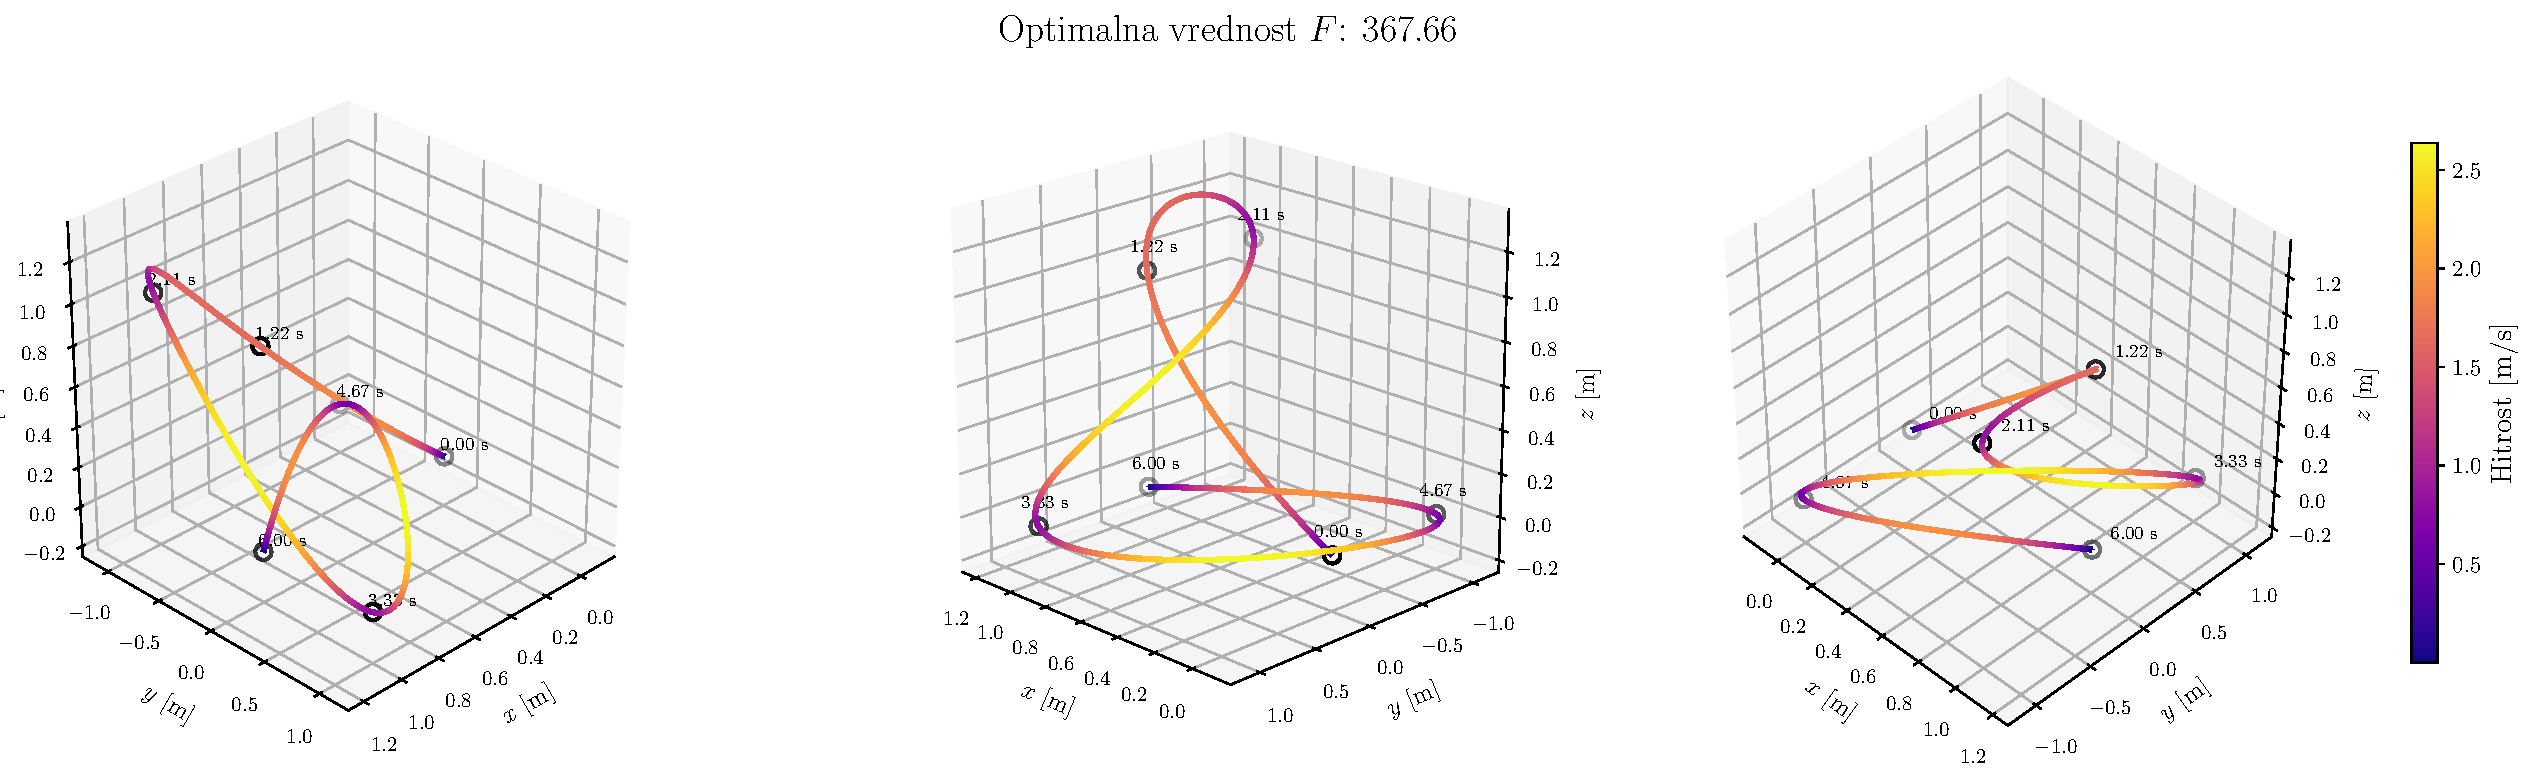
\includegraphics[width=0.99\textwidth]{images/trajectory_3d_velocity.pdf}
  \caption[Primer trajektorije.]{Primer optimalne trajektorije glede na trzaj (3. odvod) in s končnim časom 6 s, kjer so s črnimi krogi podane vmesne točke, ob njih pa so pripisani pripadajoči vmesni časi.}
  \label{fig:primer_trajektorije}
\end{figure}
% 3. luknja v raziskovanju
% 4. contributions
Doprinosi tega magistrskega dela so sledeči:
\begin{itemize}
    \item razvijemo metodo računanja drugih parcialnih odvodov optimalne rešitve spodnjega nivoja dvonivojskega optimizacijskega problema, kar nam omogoči uporabo Newtonove metode za optimizacijo zgornjega nivoja;

    \item izkoristimo bločno strukturo matrik cenovne funkcije in linearnih omejitev ter njunih odvodov, da dosežemo dodatne pohitritve;
    
    \item z eksperimenti pokažemo, da metoda skonvergira k lokalno optimalni rešitvi v manj korakih kot gradientni spust ne glede na stopnjo polinomov, optimizirane vrednosti ali števila segmentov;

    \item nadalje ugotovimo, da je Hessova matrika skoraj pasovna in da pri izračunu zgolj nekaj pasov Hessove matrike dosežemo pohitritev metode, pri čemer je vpliv izgube izvenpasovnih elementov Hessove matrike na konvergenco zanemarljiv.
\end{itemize}

\paragraph{Dostopnost implementacije.}
Implementacija metode, opisane v tem delu, je javno dostopna na GitHub repozitoriju: 

\url{https://github.com/maticpokorn/trajectory_optimization}.

% 5. opis preostanka magistrske

Preostanek tega magistrskega dela je strukturiran na sledeči način. Najprej v poglavju~\ref{sec:pregled_podrocja} opišemo sorodna dela ter dela in pojme, ki služijo kot temelj naši metodi. Nato v poglavju~\ref{sec:opis_metode} predstavimo optimizacijski problem in podrobno opišemo našo metodo reševanja in jo teoretično podkrepimo. V poglavju~\ref{sec:eksperimenti} analiziramo implementacijo naše metode v smislu konvergence in hitrosti v odvisnosti od vhodnih parametrov. V poglavju~\ref{sec:zakljucek} povzamemo vsebino in predlagamo izboljšave in nadaljnje delo. V dodatki~\ref{app:example} predstavimo del naše metode na konkretnem primeru, v dodatku~\ref{app:implementation} pa podrobno predstavimo učinkovit izračun parcialnih odvodov cenovne funkcije.



\section{Pregled področja}
\label{sec:pregled_podrocja}

V tem poglavju opišemo sorodna dela in predstavimo pojme in dognanja, na katerih je naše delo osnovano. Najprej podamo opis diferencialno ploščatih sistemov in njihovo povezavo z optimizacijo trajektorij. Nato predstavimo trenutno stanje področja optimizacije trajektorij za kvadrotorje in raziskave, na katerih naše delo bodisi temelji, bodisi predstvaljajo alternativne pristope k reševanju podobnih problemov. Potem opišemo področje dvonivojske optimizacije, na koncu pa še Newtonovo metodo za iskanje ekstremov.

\subsection{Diferencialno ploščati sistemi}
V tem delu se opiramo na pojem diferencialne ploščatosti. Sistem upravljanja
\begin{equation}
    \dot{x} = f(x, u), \quad x \in \mathbb{R}^n, u \in \mathbb{R}^m
\end{equation}
je diferencialno ploščat, če lahko najdemo tak nabor izhodnih spremenljivk $y \in \mathbb{R}^m$ (ploščati izhodi), da lahko stanje $x$ in krmilni vhod $u$ izrazimo kot funkciji ploščatih izhodov in njihovih odvodov \cite{murray1995differential}:
\begin{align}
    x &= \phi(y, \dot{y}, \ddot{y}, \dots, y^{(p)}) \\
    u &= \psi(y, \dot{y}, \ddot{y}, \dots, y^{(q)}).
\end{align}

Diferencialno ploščati sistemi upravljanja so koristni v primerih, kot je naš, kjer želimo eksplicitno določiti trajektorije. Tako lahko iz dovolj gladke trajektorije (izhoda) preprosto zračunamo vhod in stanje sistema. Izkaže se, da so tudi kvadrotorji diferencialno ploščati sistemi; postopek prevedbe iz izhodov na vhode sistema kvadrotorja je opisan v \cite{mellinger2011minimum}. V tem delu se osredotočimo na generiranje optimalnih trajektorij, diferencialna ploščatost pa je pomembna, ker želimo, da sistem trajektoriji dejansko sledi.

Pomemben vidik je tudi konstrukcija krmilnih sistemov za kvadrotorje. Obstajajo različni pristopi, kot so \ac{PID} krmilniki, \ac{LQR}, \acs{MPC} in \acs{DFBC} \cite{lee2010geometric}. Za diferencialno ploščate sisteme, kot so kvadrotorji, in agresivne manevre, so najbolj primerni nelinearni \ac{MPC} krmilniki in \ac{DFBC} krmilniki \cite{sun2022comparative}, saj lahko upoštevajo omejitve sistema in zagotavljajo stabilnost. \ac{MPC} krmilniki optimizirajo krmilne vhode na vsakem časovnem koraku glede na napovedano prihodnost, medtem ko \ac{DFBC} krmilniki neposredno izračunajo krmilne vhode iz trajektorije, kar omogoča hitro odzivanje in sledenje trajektoriji. V zadnjih letih se pojavljajo tudi krmilniki, ki uporabljajo metode strojnega učenja, kot so spodbujevano učenje (reinforcement learning) \cite{hwangbo2017control} ali odvedljivi \ac{MPC} krmilniki \cite{amos2018differentiable}.

V tem delu se osredotočamo na generiranje optimalnih trajektorij, ki so nato lahko uporabljene z različnimi krmilnimi sistemi, vključno z \ac{MPC} in \ac{DFBC} krmilniki, odvisno od specifičnih zahtev aplikacije in želene ravni nadzora nad sistemom.

\begin{comment}
\subsection{Prevedba na vhode kvadrotorja}
Kot ploščate izhode sistema si izberemo $x$-koordinato, $y$-koordinato, $z$-koordinato in $\psi$ (kot usmerjenosti) kvadrotorja, $y = [x, y, z, \psi]^T$. Najprej bomo izračunali rotacijsko matriko $R$ kvadrotorja, ki predstavlja rotacijo iz koordinatnega sistema sveta v koordinatni sistem kvadrotorja.

Premik $y$-osi izračunamo iz enačbe:
\begin{equation}
m a = 
\end{equation}

Definirajmo vmesni vektor $\mathbf{x}_c = [\cos(\psi), \sin(\psi), 0]^\top$, ki kaže v smeri kvadrotorjevega sprednjega dela.
\end{comment}

\subsection{Optimizacija trajektorij brezpilotnikov}
Načrtovanje trajektorij brezpilotnikov s polinomskimi zlepki se je uveljavilo v \cite{mellinger2011minimum}, kjer so problem s fiksno razporeditvijo časa po segmentih definirali kot \ac{QP}. Kasneje so v \cite{richter2016polynomial} izboljšali numerično stabilnost te metode tako, da so enakostne omejitve vključili v cenovno funkcijo, v \cite{burke2020generating} pa so se osredotočili na pohitritev in pokazali linearno časovno zahtevnost v odvisnosti od števila segmentov. V \cite{mellinger2011minimum} so predstavili tudi problem, kjer optimizirajo časovno razporeditev po segmentih; optimizacijo izvedejo z gradientnim spustom, kjer pa gradient izračunajo z metodo končnih diferenc, ki pa za izračun gradienta zahteva linearno mnogo rešitev \ac{QP} v razmerju s številom segmentov. Ta problem rešijo v \cite{sun2021fast}, kjer gradient izračunajo analitično z občutljivostno analizo \ac{KKT} \ac{QP}. V \cite{gao2018online} čase segmentov določijo hevristično. V \cite{wang2021generating} problem s fiksnimi časi segmentov rešijo z dvojnim opisovanjem polinomov in dosežejo izjemne pohitritve.

V optimizaciji trajektorij pomembno vlogo igrajo neenakostne omejitve za izogibanje oviram in omejevanje maksimalne hitrosti, pospeška, itd. Za izogibanje oviram se pogosto uporabljajo pristopi, ki uporabljajo zaporedja konveksnih poliedrov, da ustvarijo varne koridorje letenja; obstajajo algoritmi, ki učinkovito izračunajo včrtan polieder okoli točke \cite{deits2015computing} oz. daljice \cite{liu2017planning}. Na ta način neenakostne omejitve za izogibanje oviram uporabijo v \cite{sun2021fast}, kjer kasneje optimizirajo časovno razporeditev po segmentih. V \cite{tordesillas2021faster} namesto optimizacije časov segmentov problem formulirajo kot mešan celoštevilski kvadratni program (MIQP), kjer fiksirajo čase segmentov in uporabijo diskretne spremenljivke, da določijo, kateri segmenti se bodo nahajali v katerem poliedru.

Algoritmi, ki optimizacijo polinomskih trajektorij rešujejo s \ac{QP}, pogosto uporabljajo različne baze polinomov, kot so Bernsteinovi polinomi \cite{sun2021fast, tordesillas2021faster} in B-zlepki \cite{zhou2020ego}, kar omogoča enostavno vključevanje neenakostnih omejitev s kontrolnimi točkami in boljšo numerično stabilnost v primerjavi z običajnimi monomskimi polinomi \cite{runge1901}. Kljub prednostim Bernsteinovih polinomov in B-zlepkov tem delu uporabljamo monomske polinome, saj nam to omogoči enostavnejšo izpeljavo analitičnih odvodov drugega reda, kar je ključno za našo metodo.

Obstajajo tudi pristopi, ki ne ločijo časovnih in prostorskih spremenljivk \cite{fridovich2018planning} in se zanašajo na kompleksne algoritme za nelinearno programiranje \cite{wachter2006implementation}. Ti algoritmi pogosto omogočajo sočasno optimizacijo vmesnih točk znotraj določenega dopustnega območja, kar poveča prilagodljivost trajektorije.

Pristopi za optimizacijo trajektorij se srečujejo z dilemo, kjer morajo najti ravnovesje med hitrostjo izračuna in optimalnostjo rezultata. V \cite{zhou2020ego} se osredotočajo na hitrost in trajektorije izračunajo v milisekundah, vendar ne zagotavljajo optimalnosti, kar lahko povzroči bolj agresivne manevre in posledično neučunkovite in nevarne trajektorije. V \cite{richter2016polynomial} se osredotočajo na optimalnost, vendar je čas izračuna trajektorije v sekundah, kar je neprimerno za načrtovanje trajektorij v realnem času. V tem delu zagotavljamo konvergenco k lokalno optimalni rešitvi, pri čemer želimo zagotoviti hitro izračunavanje trajektorij. Medtem ko naša metoda z obstoječo implementacijo ni dovolj hitra za načrtovanje trajektorij povsem v realnem času, je primerna za asinhrono generiranje trajektorij, kjer se trajektorije izračunajo v ločenem procesu, ki ni vezan na časovno omejitev, in se nato posredujejo v proces vodenja brezpilotnika, ki sledi trajektoriji.

\subsection{Dvonivojska optimizacija}
Dvonivojska optimizacija se ukvarja z optimizacijskimi problemi, kjer je cenovna funkcija enega optimizacijskega problema (zgornji nivo) odvisna od optimalne vrednosti odločitvenih spremenljivk drugega optimizacijskega problema (spodnji nivo). Splošna oblika dvonivojskega optimizacijskega problema je predstavljena kot:
\begin{equation}
    \begin{aligned}
        \min_{x\in X, y^*\in Y}& \quad F(x,y^*) \\
        \text{p.p.} & \quad y^* = \arg \min_{y\in Y} \{f(y) : g(x,y) \leq 0\} \\
        &\quad G(x,y^*) \leq 0,
    \end{aligned}
\end{equation}
kjer sta $f$ in $g$ cenovna funkcija in omejitve spodnjega nivoja, $F$ in $G$ pa cenovna funkcija in omejitve zgornjega nivoja.

Znan primer dvonivojske optimizacije je Stacklebergova igra \cite{stackelberg1934marktform}, ki je igra med dvema igralcema (voditelj in sledilec), kjer voditelj optimizira svojo strategijo glede na sledilčevo. 

Dvonivojska optimizacija v načrtovanju trajektorij brezpilotnikov in v robotiki na splošno se navadno uporablja, ko je optimizacijski problem odvisen od časovne razporeditve in nekaterih drugih parametrov, ki pa so tudi odvisni od časovne razporeditve. V našem primeru so to koeficienti polinomov. Pogosto se, kot v našem primeru, izkaže, da se da spodnji nivo izraziti kot \ac{QP}, ki se ga da rešiti s standardnimi knjižnicami. Tudi problem v \cite{mellinger2011minimum} je implicitno definiran kot dvonivojski optimizacijski problem. V \cite{sun2021fast} poleg izračuna analitičnih gradientov svojo rešitev podkrepijo teoretično. Izven domene načrtovanja trajektorij v \cite{amos2017optnet} dvonivojsko optimizacijo na \ac{QP} uporabijo za integracijo \ac{QP} kot plast v golobkih nevronskih mrežah, kjer so parametri \ac{QP} odvisni od drugih plasti v nevronski mreži. V \cite{dyro2022second} razvijejo teorijo računanja Hessove matrike zgornjega problema splošnih dvonivojskih neomejenih optimizacijskih problemov z uporabo \acl{IIF} (\acs{IIF}); z eksperimenti tudi pokažejo hitrejšo konvergenco kot obstoječe metode.

%Poleg robotike se dvonivojska optimizacija aplikativno uporablja tudi v ekonomiji

\subsection{Newtonova metoda}
Newtonova metoda je iterativna metoda za iskanje ekstremov dvakrat zvezno odvedljivih funkcij \cite{newton1736method, boyd2004convex}. Korak v iteraciji Newtonove metode za funkcije več spremenljivk se izračuna z enačbo

\begin{equation}
    x_{k+1} = x_k - [\nabla^2_f(x_k)]^{-1} \nabla_f(x_k), 
\end{equation}
kjer je $f : \mathbb{R}^n \to \mathbb{R}$ dvakrat zvezno odvedljiva funkcija, $x_k \in \mathbb{R}^n$ trenutna točka, $x_{k+1} \in \mathbb{R}^n$ pa naslednja točka iteracije. $\nabla^2_f(x_k)$ predstvavlja Hessovo matriko funkcije $f$ v točki $x_k$, $\nabla_f(x_k)$ pa gradient funkcije $f$ v točki $x_k$. Kot že omenjeno, v \cite{dyro2022second} razvijejo teorijo računanja gradienta in Hessove matrike za neomejene dvonivojske optimizacijske probleme in pokažejo hitro konvergenco. Tudi v tem delu eksperimenti pokažejo zelo hitro konvergenco k optimalni rešitvi.

\section{Opis metode}
\label{sec:opis_metode}

V tem poglavju opišemo našo metodo. Najprej definiramo osnovni problem v obliki minimizacije funkcionala z omejitvami s fiksnimi potovalnimi časi po segmentih. Nato pokažemo, kako se problem minimizacije funkcionala prevede na QP, kjer optimizacijske spremenljivke postanejo koeficienti polinomov. Dodamo optimizacijo po časih segmentov in predstavimo glavni optimizacijski problem, ki ga v tem delu rešujemo. Nato opišemo, kako lahko s pomočjo KKT pogojev QP izluščimo gradient in Hessovo matriko cenovne funkcije v zgornjem nivoju dvonivojskega problema. Zatem predstavimo minimizacijski algoritem, ki sloni na Newtonovi metodi. Na koncu pokažemo, kako lahko z uporabo bločne strukture matrik in strukture Hessove matrike dosežemo velike pohitritve. 

Najprej pa uvedemo nekaj nestandardne notacije, ki bo služila za boljšo preglednost in razumljivost v enačbah v tem poglavju:

Naj bo $\mathbf{A}(\mathbf{t}) \in \mathcal{C}^2(\mathbb{R}^k, \mathbb{R}^{m\times n})$ matrika, kjer je vsak element dvakrat zvezno odvedljiva funkcija vektorja $\mathbf{t}$.
\begin{itemize}
    \item S simbolom $\partial_{t_i} \mathbf{A}$ označimo matriko parcialnih odvodov glede na $i$-to komponento vektorja $\mathbf{t}$:
    \begin{equation} \partial_{t_i} \mathbf{A} := \frac{\partial \mathbf{A}(\mathbf{t})}{\partial t_i} = \left[ \frac{\partial a_{uv}(\mathbf{t})}{\partial t_i} \right]_{u,v=1}^{m,n} \end{equation}
    \item V nadaljevanju bomo zaradi večje preglednosti izpeljav pogosto opuščali eksplicitno navajanje argumenta $\mathbf{t}$ (npr. $\mathbf{A}$ namesto $\mathbf{A}(\mathbf{t})$), razen v primerih, ko je to nujno za razumevanje.
\end{itemize}


\subsection{Problem s podanimi časi segmentov}
Rešujemo spodnji problem:

Definirano imamo zaporedje vmesnih točk $P_0, \ldots P_n$ in potovalne čase za posamezen segment $t_1, \ldots, t_n$. Najti moramo polinome $p_1, \ldots, p_n$, ki minimizirajo spodnji funkcional:

\begin{equation}
\label{eq:functional}
\begin{aligned}
    \min_{p_1, \ldots p_n}& \quad \sum_{i=1}^n \int_0^{t_i} (p_i^{(r)}(\tau))^2 d\tau \\
    \text{p.p.} & \quad p_1(0) = P_0, \quad p_n(t_n) = P_n& \\
    & \quad p^{(k)}_1(0) = 0 \quad ; \quad &k = 1, \ldots, K \\
     &\quad p^{(k)}_n(t_n) = 0 \quad ; \quad &k = 1, \ldots, K \\
     \quad &p_i(t_i) = p_{i+1}(0) = P_i \quad ;& \quad i = 1, \ldots , n-1 \\
     \quad &p_i^{(k)}(t_i) = p_{i+1}^{(k)}(0) \quad ; \quad &i = 1, \ldots, n-1,\quad k = 1, \ldots, K 
\end{aligned}
\end{equation}
Pravzaprav tak problem rešujemo trikrat, posebej za vsako od osi $x$, $y$ ter $z$, kjer $t_i$ ostane isti, spremenijo pa se zgolj koordinate vmesnih točk $P_i$ za posamezno os. Z nekaj svobode pa lahko izberemo parametre:
\begin{itemize}
    \item $d$, stopnja polinomskih zlepkov
    \item $K$, red zveznosti trajektorije
    \item $r$, optimizacijska stopnja odvoda
\end{itemize}
%Veljati mora $r \leq k \leq d$, standardne vrednosti pa so $d = 9$, $r = 3$ (trzaj) ali $r = 4$ (pok) ter $k = r$.

\subsection{Prevedba na \acs{QP}}
\label{sec:prevedba}

V tem razdelku opišemo, kako problem, predstavljen v ~\eqref{eq:functional} prevedemo na \ac{QP} oblike:
\begin{equation}
    \begin{aligned}
        &\frac{1}{2}\mathbf{a}^\top \mathbf{Q} \mathbf{a}\\
        \text{p.p.}\quad & \mathbf{A}\mathbf{a} = \mathbf{b},
    \end{aligned}
\end{equation}
kjer je $\mathbf{a} \in \mathbb{R}^{n (d+1)}$ optimizacijski vektor in predstavlja koeficiente polinomskih zlepkov, $\mathbf{Q} \in \mathbb{R}^{n(d+1) \times n(d+1)}$ je simetrična in pozitivno definitna matrika, $\mathbf{A} \in \mathbb{R}^{M \times n(d+1)}$ in $\mathbf{b} \in \mathbb{R}^M$ pa predstavljata linearne omejitve. Najprej bomo pokazali, kako izračunamo matriko $\mathbf{Q}$, nato pa še, kako izračunamo matriko $\mathbf{A}$ in vektor $\mathbf{b}$. Bistvenega pomena pri tej izpeljavi je, da so elementi matrik $\mathbf{Q}$ in $\mathbf{A}$ zvezno odvisni od vmesnih časov $t_i$ \cite{carlone2020vnav}.

\subsubsection{Izračun matrike $\mathbf{Q}$}
Matriko $\mathbf{Q}$ izračunamo tako, da ločeno prevedemo posamezen integral $\int_0^{t_i} (p_i^{(r)}(\tau))^2 d\tau$ na matrično enačbo $\mathbf{a}_i^\top \mathbf{Q}_i \mathbf{a}_i$, kjer je $\mathbf{a}_i$ vektor koeficientov $i$-tega polinoma. Celotno vsoto $\sum_{i=1}^n \int_0^{t_i} (p_i^{(r)}(\tau))^2 d\tau$ pa nato predstavimo kot bločno matriko
\begin{equation}
\label{eq:cost_function_matrix}
    \mathbf{a}^\top \mathbf{Q} \mathbf{a} = 
    \begin{bmatrix}
        \mathbf{a}_1 \\ \mathbf{a}_2 \\ \vdots \\ \mathbf{a}_n 
    \end{bmatrix}^\top
    \begin{bmatrix}
        \mathbf{Q}_1 & \mathbf{0} & \cdots & \mathbf{0} \\
        \mathbf{0} & \mathbf{Q}_2 & \cdots & \mathbf{0} \\
        \vdots & \vdots & \ddots & \vdots \\
        \mathbf{0} & \mathbf{0} & \cdots & \mathbf{Q}_n
    \end{bmatrix}
    \begin{bmatrix}
        \mathbf{a}_1 \\ \mathbf{a}_2 \\ \vdots \\ \mathbf{a}_n 
    \end{bmatrix}
\end{equation}

Za preoblikovaje integrala $J := \int_0^{t_i} (p_i^{(r)}(\tau))^2 d\tau$ v matrično obliko uporabimo naslednja rezultata:
\begin{enumerate}
    \item \textbf{$r$-ti odvod polinoma.}
\begin{equation}
    p^{(r)}(\tau) = \sum_{k=r}^{d} \left[\prod_{m=0}^{r-1} (k-m)\right]a_{k} \tau^{k-r}
\end{equation}
    \item \textbf{Kvadrat polinoma.}
    \begin{equation}
        p(\tau)^2 = \sum_{k=0}^{2d} \left( \sum_{l=0}^{d} a_l a_{k-l} \right) \tau^k
    \end{equation}
    Tu predpostavimo, da so koeficienti, kjer je indeks večji od stopnje polinoma ali manjši od 0, enaki 0.
\end{enumerate}

Z združitvijo zgornjih rezultatov lahko izrazimo integrand $(p^{(r)}(\tau))^2$ kot:
\begin{equation}
    (p^{(r)}(\tau))^2 = \sum_{k=0}^{2d} \left( \sum_{l=r}^{d} \prod_{m=0}^{r-1} (l-m)(k-l-m) a_l a_{k-l} \right) \tau^{k-2r}
\end{equation}

Sedaj pa lahko izračunamo integral:
\begin{equation}
    \int_0^{t_i} (p^{(r)}(\tau))^2 d\tau = \sum_{k=0}^{2d} \left( \sum_{l=r}^{d} \prod_{m=0}^{r-1} (l-m)(k-l-m) a_l a_{k-l} \right) \frac{t_i^{k-2r+1}}{k-2r+1}
\end{equation}

Sedaj že lahko opazimo, da imajo posamezni členi v vsoti obliko $\qmat_{uv} a_u a_v$ za neke $\qmat_{uv}$. Vendar pa koeficienti $a_u$ in $a_v$ nastopajo v različnih členih vsote. Zato $\qmat_{uv}$ izračunamo tako, da izračunamo parcialne odvode drugega reda funkcije $J$. S tem členi vsote, ki ne vsebujejo $a_u a_v$, postanejo ničelni, medtem ko vsota členov, ki vsebujejo $a_u a_v$, postane $\qmat_{uv}$:
\begin{equation}
    \qmat_{uv} = \frac{\partial^2 J}{\partial a_u \partial a_v}
\end{equation}

Najprej izračunamo parcialni odvod prvega reda funkcije $J$:
\begin{equation}
    \begin{aligned}
    \frac{\partial J}{\partial a_u} &= \sum_{k=0}^{2d} \sum_{l=0}^{d} \prod_{m=0}^{r-1} (l-m)(k-l-m) \left(\frac{\partial a_l}{\partial a_u} a_{k-l} + \frac{\partial a_{k-l}}{\partial a_u} a_l \right) \frac{t^{k-2r+1}}{k-2r+1}\\
    &= 2\sum_{k=0}^{2d} \prod_{m=0}^{r-1} (u-m)(k-u-m) a_{k-u} \frac{t^{k-2r+1}}{k-2r+1}
\end{aligned}
\end{equation}

Pri odvajanju notranje vsote dobimo samo dva neničelna člena, kjer je $0 \leq u \leq d$. Sedaj dobljeno funkcijo odvajamo še enkrat po $a_v$:

\begin{equation}
\begin{aligned}
    \frac{\partial^2 J}{\partial a_u \partial a_v} &= 2\sum_{k=0}^{2d} \prod_{m=0}^{r-1} (v-m)(k-v-m) \frac{\partial a_{k-v}}{\partial a_u} \frac{t^{k-2r+1}}{k-2r+1}\\
    &= 2\prod_{m=0}^{r-1} (v-m)(u-m) \frac{t^{v+u-2r+1}}{v+u-2r+1}
\end{aligned}
\end{equation}

Pri drugem parcialnem odvodu preostale vsote pa pa dobimo samo en neničelen člen, kjer $v = k-u$ in $0 \leq v \leq d$.

Torej lahko zaključimo, da velja:
\begin{equation}
    \qmat_{uv} = \begin{cases}
        \prod_{m=0}^{r-1} (u - m)(v - m) \dfrac{t^{u+v-2r+1}}{u + v - 2r + 1} & u, v \geq r\\
        0 & \text{sicer}
    \end{cases}, \quad \text{in} \quad \qmat_{vu} = \qmat_{uv}
\end{equation},

funkcijo $J$ pa lahko izrazimo kot $J = \sum_{uv} \qmat_{uv} a_u a_v = \avec^\top \qmat \avec$.

S tem smo preoblikovali ciljni funkcional v kvadratno funkcijo koeficientov polinoma.

\subsubsection{Izračun matrike $\amat$ in vektorja $\bvec$}

Matriko $\amat$ in vektor $\bvec$ izračunamo tako, da prevedemo linearne omejitve problema~\eqref{eq:functional} na matrično obliko $\amat \avec = \bvec$. Vsaka linearna omejitev v problemu~\eqref{eq:functional} se prevede v vrstico matrike $\amat$ in ustrezen element vektorja $\bvec$. Tako kot matrika $\qmat$ ima tudi $\amat$ bločno strukturo, in sicer:
\begin{equation}
    \amat(\tvec) = 
    \begin{bmatrix}
    \amat_1(0) & \mathbf{0} & \mathbf{0} & \cdots & \mathbf{0} & \mathbf{0} \\
    \amat_1(t_1) & -\amat_2(0) & \mathbf{0} & \cdots & \mathbf{0} & \mathbf{0} \\
    \mathbf{0} & \amat_2(t_2) & - \amat_3(0) & \cdots & \mathbf{0} & \mathbf{0} \\
    \vdots & \vdots & \ddots & \ddots & \vdots & \vdots \\
    \mathbf{0} & \mathbf{0} & \mathbf{0} &\cdots & \amat_{n-1}(t_{n-1}) & \amat_n(0) \\
    \mathbf{0} & \mathbf{0} & \mathbf{0} &\cdots & \mathbf{0} & \amat_n(t_n)
    \end{bmatrix}
\end{equation}

Sedaj pokažemo, kako so strukturirane posamezne komponente matrike $\amat$. Ločeno pozornost posvetimo začetnemu bloku $\amat_1(0)$, končnemu bloku $\amat_n(t_n)$ in vmesnim parom blokov $\amat_i(t_i)$ in $-\amat_{i+1}(0)$, kjer $i = 1, \ldots, n-1$:

\begin{itemize}
\item Začetni blok $\amat_1(0)$ predstavlja omejitve začetka trajektorije, ki zahtevajo, da $p_1(0) = P_0$ in $p_1^{(k)}(0) = 0$ za $k = 1, \ldots, K$. 

\item Končni blok $\amat_n(t_n)$ predstavlja omejitve konca trajektorije, ki zahtevajo, da $p_n(t_n) = P_n$ in $p_n^{(k)}(t_n) = 0$ za $k = 1, \ldots, K$.


\item Vmesni pari blokov $\amat_i(t_i)$ in $-\amat_{i+1}(0)$ predstavljajo omejitve zveznosti trajektorije na vmesnih točkah, ki zahtevajo, da $p_i(t_i) = p_{i+1}(0) = P_i$ in $p_i^{(k)}(t_i) = p_{i+1}^{(k)}(0)$ za $k = 1, \ldots, K$ in $i = 1, \ldots, n-1$.
\end{itemize}

Podrobnejši primer konstrukcije QP s fiksnimi časi segmentov je podan v dodatku~\ref{app:example}.


\subsection{Problem s časovnimi spremenljivkami}

\begin{figure}
     \centering
     \begin{subfigure}[b]{0.48\textwidth}
         \centering
         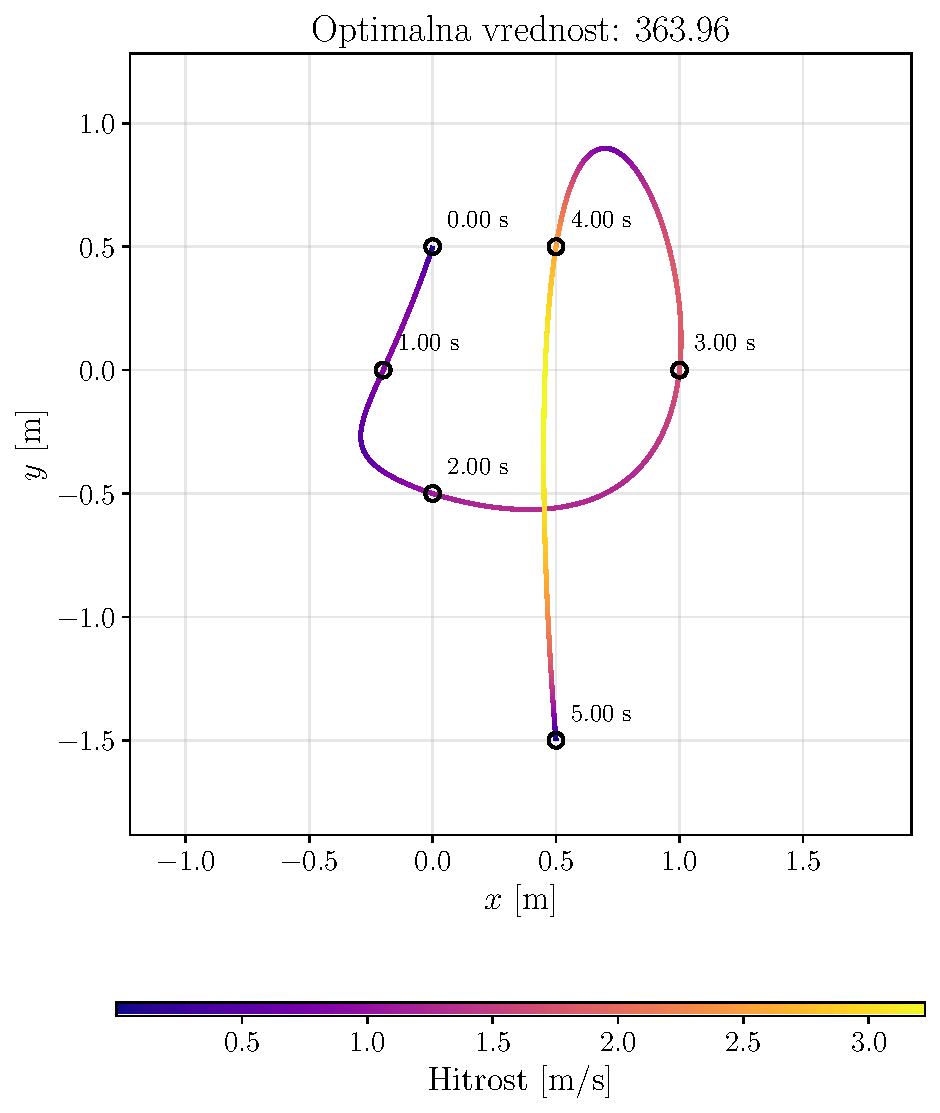
\includegraphics[width=\textwidth]{images/phi_fixed_time.pdf}
         \caption{Trajektorija s fiksno določenimi vmesnimi časi (vsak segment 1s) - izračunana s QP.}
         \label{fig:fixed_time}
     \end{subfigure}
     \hfill
     \begin{subfigure}[b]{0.48\textwidth}
         \centering
         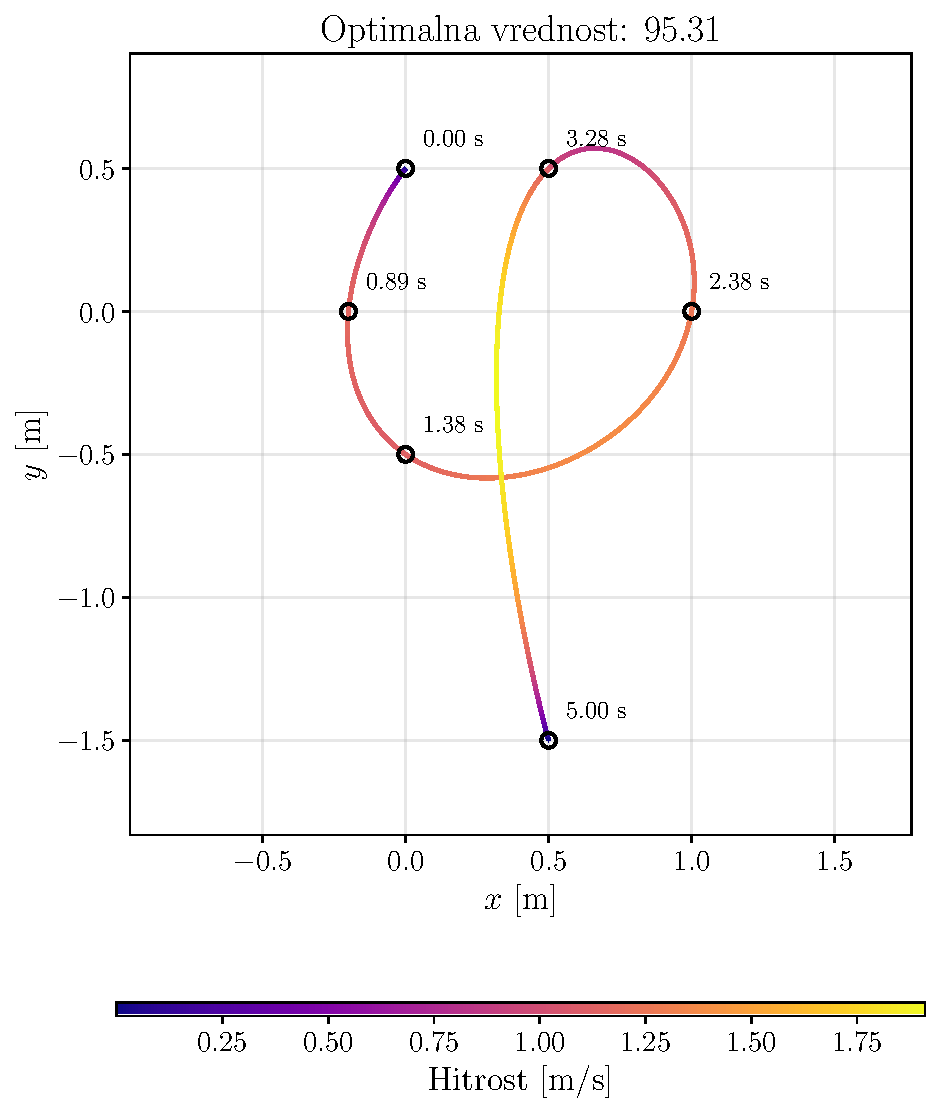
\includegraphics[width=\textwidth]{images/phi_variable_time.pdf}
         \caption{Trajektorija z optimiziranimi vmesnimi časi - izračunana z dvonivojsko optimizacijo.}
         \label{fig:variable_time}
     \end{subfigure}
     \caption{Primerjava trajektorij, kjer fiksno določimo vmesne čase (a), in kjer izvedemo optimizacijo po vmesnih časih (b). Obe trajektoriji imata končni čas 5s, vendar ima desna trajektorija nižjo optimialno vrednost in tudi nižjo maksimalno hitrost.}
     \label{fig:primerjava_fixed_variable}
\end{figure}

V prejšnjem poglavju smo predstavili problem, kjer so časi segmentov podani kot fiksni parametri problema. Pogosto pa nam je pomemben le celoten čas potovanja po trajektoriji. Na primer, slika~\ref{fig:primerjava_fixed_variable} nudi primerjavo med fiksno določenimi vmesnimi časi in optimiziranimi vmesnimi časi za isto zaporedje vmesnih točk in isti skupen čas. Če nam je vseeno, kakšni so časi na vmesnih točkah, je očitno, da optimizacija časov segmentov vodi do bistveno boljše trajektorije. Zato lahko definiramo želen skupen čas trajektorije $T$ in vektor spremenljivk $\mathbf{t} = \left[ t_1, t_2, \ldots , t_n\right]$, kjer velja $\sum_{i=1}^n t_i = T$ in $t_i > 0$.  Sedaj lahko formuliramo nov optimizacijski problem:

\begin{equation}
    \begin{aligned}
        \min_{\mathbf{t},\mathbf{a}} & \quad \frac{1}{2}\mathbf{a}^\top \mathbf{Q}(\mathbf{t}) \mathbf{a}\\
        \text{p.p.} & \quad \mathbf{A}(\mathbf{t})\mathbf{a} = \mathbf{b}\\
        & \quad \mathbf{t} > \mathbf{0} \\
        & \quad \mathbf{1}^\top \mathbf{t} = T,
    \end{aligned}
\end{equation}
kjer je $\mathbf{1}$ vektor enic. Očitno je, da ta problem ni konveksen, niti nima konveksnih omejitev. Zato ga je koristno reformulirati v sledečo ekvivalentno dvonivojsko obliko:

\begin{equation}
    \label{eq:bilevel}
    \begin{aligned}
        \min_{\mathbf{t},\mathbf{a^*}}& \quad F(\mathbf{t}) := \frac{1}{2}\mathbf{a^{*\top}}\mathbf{Q}(\mathbf{t})\mathbf{a^*} \\
        \text{p.p.}& \quad\mathbf{a^*} = \arg \min_\mathbf{a} \{\frac{1}{2}\mathbf{a}^\top\mathbf{Q}(\mathbf{t})\mathbf{a} : \mathbf{A}(\mathbf{t})\mathbf{a} = \mathbf{b}\}\\
        & \quad \mathbf{t} > \mathbf{0} \\
        & \quad \mathbf{1}^\top \mathbf{t} = T,
    \end{aligned}
\end{equation}

kjer problemu računanja $\mathbf{a}^*$ rečemo spodnji nivo dvonivojskega optimizacijskega problema, problemu minimizacije $F(\mathbf{t})$ pa zgornji nivo. Če fiksiramo $\mathbf{t}$, je spodnji nivo preprost QP z enakostnimi omejitvami. S takim problemom se srečujejo v \cite{mellinger2011minimum, sun2021fast}, kjer v neki točki $\mathbf{t}'$ izračunajo gradient $\nabla_\mathbf{t}F(\mathbf{t}')$ in izvedejo gradientni spust. Pri tem za izračun gradienta v \cite{mellinger2011minimum} uporabijo metodo končnih diferenc, v \cite{sun2021fast} pa ga izračunajo analitično.

To je glavni optimizacijski problem, s katerim se v tem magistrskem delu ukvarjamo in preostanek tega poglavja je posvečen opisu naše metode njegovega reševanja. V naslednjem podpoglavju s pomočjo KKT pogojev in izreka o implicitni funkciji pokažemo, da za vsak $\tvec$ obstaja funkcija $\aimplicit \in \mathcal{C}^\infty$, kjer $\aimplicit(\tvec) = \mathbf{a}^*$. S tem pokažemo, da velja tudi $F \in \mathcal{C}^\infty$ in omogočimo izračun analitičnih parcialnih odvodov višjega reda za $F(\mathbf{t})$ in s tem gradienta in Hessove matrike.

%Dodatno, $\mathbf{Q}, \mathbf{A} \in \mathcal{C}^{\infty}(\mathbb{R}^n)$.

\subsection{Odvajanje s \acs{KKT} pogoji}

V tem podpoglavju bomo predstavili, kako s pomočjo \ac{KKT} izračunamo gradient in Hessovo matriko cenovne funkcije zgornjenivojskega problema. Najprej predstavimo izrek o \ac{KKT} za splošen optimizacijski program in opišemo lastnosti \ac{KKT}, če imamo konveksen optimizacijski program. Nato v~\ref{eq:kkt_matrix} definiramo \acs{KKT} matriko za \ac{QP} z enakostnimi omejitvami. V~\ref{sec:ift} navedemo \acl{IIF} in pokažemo, da obstaja analitična funkcija $\aimplicit$, kjer velja $\aimplicit(\tvec) = \mathbf{a}^*$. S tem argumentiramo izračun parcialnih odvodov $\aimplicit$ ter gradienta in Hessove matrike, ki jih predstavimo v~\ref{sec:grad} in~\ref{sec:hess}.

Spodaj navedemo standarden izrek o \ac{KKT} \cite{bertsekas1997nonlinear}.

\textbf{Karush-Kuhn-Tuckerjevi pogoji.} Za optimizacijski program
\[
\min_x f(x) \quad \text{p.p.} \quad g_i(x) \leq 0, \ i=1,\dots,m, \quad h_j(x) = 0, \ j=1,\dots,p,
\]
so Karush-Kuhn-Tuckerjevi pogoji naslednji: obstajajo Lagrangeevi multiplikatorji $\lambda \in \mathbb{R}^m_{\geq 0}$, $\mu \in \mathbb{R}^p$, da velja
\begin{align}
\nabla f(x) + \sum_{i=1}^m \lambda_i \nabla g_i(x) + \sum_{j=1}^p \mu_j \nabla h_j(x) &= 0, \label{eq:kkt-stationarity} \\
\lambda_i g_i(x) &= 0, \quad i=1,\dots,m, \label{eq:kkt-complementarity} \\
g_i(x) &\leq 0, \quad i=1,\dots,m, \label{eq:kkt-primal-feasibility} \\
h_j(x) &= 0, \quad j=1,\dots,p, \label{eq:kkt-equality} \\
\lambda &\geq 0. \label{eq:kkt-dual-feasibility}
\end{align}

Za \emph{konveksne programe}, kjer je $f$ konveksna, $g_i$ konveksne, $h_j$ afine in velja Slaterjev pogoj, postanejo \ac{KKT} \emph{potrebni in zadostni} za globalno optimalnost. Slaterjev pogoj predstavimo spodaj.

\textbf{Slaterjev pogoj \cite{bertsekas1997nonlinear,boyd2004convex}.} 
Za konveksni program
\[
\min_x f(x) \quad \text{p.p.} \quad g_i(x) \leq 0, \ i=1,\dots,m, \quad h_j(x) = 0, \ j=1,\dots,p,
\]
Slaterjev pogoj velja, če obstaja $x^\circ$ tako, da
\begin{itemize}
\item $g_i(x^\circ) < 0$ za vse $i=1,\dots,m$ (stroga neenakostna dopustnost),
\item $h_j(x^\circ) = 0$ for all $j=1,\dots,p$ (enakostna dopustnost).
\end{itemize}

Opazimo lahko, da v primeru, kjer neenakostnih omejitem ni, Slaterjev pogoj velja.

\subsubsection{\acs{KKT} pogoji \acs{QP}}

V primeru našega optimizacijskega problema, kjer imamo kvadratno cenovno funkcijo in enakostne omejitve, lahko privzamemo Slaterjev pogoj, saj nimamo neenakostnih omejitev, \ac{KKT} pa se zreducirajo na:

\begin{equation}
    \begin{aligned}
        \nabla (\frac{1}{2}\mathbf{a^{*\top}}\mathbf{Q}\mathbf{a^*}) + \sum_{i=1}^m \mathbf{\mu^*}_i \nabla(\mathbf{A}_i \mathbf{a^*}) = \mathbf{0}& \\
        \mathbf{A}_i \mathbf{a^*} - \mathbf{b}_i = 0&, \quad i = 1,\ldots, m,
    \end{aligned}
\end{equation}

še bolj kompaktno pa jih lahko zapišem kot:

\begin{equation}
    \begin{aligned}
        \mathbf{Q}\mathbf{a^*} + \mathbf{A^\top}\mathbf{\mu^*} = \mathbf{0}& \\
        \mathbf{A} \mathbf{a^*} = \mathbf{b}&.
    \end{aligned}
\end{equation}

Pri optimalnosti torej velja naslednja matrična enačba, kjer so $\mathbf{\mu}$ enakostni Lagrangeevi multiplikatorji, $\mathbf{a^*}$, ter $\mathbf{\mu^*}$ pa so vrednosti $\mathbf{a}$ ter $\mathbf{\mu}$ pri optimalnosti:
\begin{equation}
    \label{eq:kkt_matrix}
    \begin{gathered}
        % Top Equation
        \underbrace{
            \begin{bmatrix}
                \qmat & \amat^{\top} \\
                \amat & \mathbf{0}
            \end{bmatrix}
        }_{\kmat}
        \underbrace{
            \begin{bmatrix}
                \avec^* \\
                \boldsymbol{\mu}^*
            \end{bmatrix}
        }_{\mathbf{y}^*}
        -
        \underbrace{
            \begin{bmatrix}
                \mathbf{0} \\
                \bvec
            \end{bmatrix}
        }_{\mathbf{c}}
        = \mathbf{0}
    \end{gathered}
\end{equation}

Spodnji optimizacijski problem v enačbi~\eqref{eq:bilevel} bi torej lahko nadomestili z zgornjo matrično enačbo. V literaturi se področju, ki se ukvarja s takimi problemi, reče tudi \acl{mpec}.

V nadaljevanju bomo izmenično uporabljali tako osnovno kot kompaktno obliko ($\kmat \mathbf{y}^* - \mathbf{c} = \mathbf{0}$) zapisa \ac{KKT}. Kompaktno obliko bomo uporabili, kjer bo to pripomoglo k boljši preglednosti, osnovno obliko pa tam, kjer bo pomembna struktura posameznih delov matrike $\kmat$, ali pa bo treba ločiti med primarnimi in dualnimi komponentami $\mathbf{y}^*$.

\subsubsection{Izrek o implicitni funkciji}
\label{sec:ift}

Z uporabo izreka o implicitni fukciji lahko pokažemo, da obstaja odprta množica $U$ in gladke funkcije $\yimplicit$ : $U \to \R^{m+n}$, $\aimplicit$ : $U \to \R^{n}$, $\muimplicit$ : $U \to \R^{m}$, kjer velja $\yimplicit(\tvec) = (\aimplicit(\tvec), \muimplicit(\tvec)) = (\avec^*, \muvec^*)$. To nam da formalno podlago, da cenovno funkcijo $F(\tvec)$ odvajamo glede na $\tvec$, saj jo lahko zapišemo kot:

\begin{equation}
    F(\mathbf{t}) = \frac{1}{2}\avec^{*\top}\qmat(\tvec)\avec^* = \frac{1}{2} \aimplicit(\tvec)^\top \qmat(\tvec) \aimplicit(\tvec)
\end{equation}

Dodatno velja:
\begin{equation}
    \label{eq:equilibrium_implicit}
    \kmat(\tvec) \mathbf(y)^* - \mathbf{c} = \kmat(\tvec) \yimplicit(\tvec) - \mathbf{c} = \mathbf{0}
\end{equation}

V tem razdelku najprej podamo izrek o implicitni funkciji \cite{lee2003smooth} in nato pokažemo, kako z njim argumentiramo obstoj gladkih funkcij $\yimplicit$, $\aimplicit$ in $\muimplicit$.

\begin{izrek}[Izrek o implicitni funkciji \cite{lee2003smooth}]
    Naj bo $f: \mathbb{R}^{m+n} \to \mathbb{R}^m$ zvezno odvedljiva funkcija in naj ima $\mathbb{R}^{m+n}$ koordinate $(\mathbf{x},\mathbf{y})$. 
    
    Fiksirajmo točko $(\mathbf{a}, \mathbf{b}) = (a_1, a_2, \ldots, a_m, b_1, b_2, \ldots, a_n)$, kjer velja $f(\mathbf{a},\mathbf{b}) = \mathbf{0}$ in $\mathbf{0} \in \mathbb{R}^m$ je ničelni vektor. Če je Jacobijeva matrika:
    \begin{equation}
        J_{f,\mathbf{y}}(\mathbf{a}, \mathbf{b}) = \left[ \frac{\partial f_i}{\partial y_j} (\mathbf{a},\mathbf{b})\right]
    \end{equation}

    obrnljiva, potem obstaja odprta množica $U \in \mathbb{R}^n$, ki vsebuje $\mathbf{a}$, tako da obstaja enolična funkcija $g:U \to \mathbb{R}^m$, kjer $g(\mathbf{a}) = \mathbf{b}$ in $f(\mathbf{x}, g(\mathbf{x})) = \mathbf{0}$ za vse $\mathbf{x} \in U$. Nadalje, $g$ je zvezno odvedljiva in Jacobijeva matrika parcialnih odvodov $g$ v $U$ je definirana kot:
    \begin{equation}
        \left[\frac{\partial g_i}{\partial x_j}(\mathbf{x})\right]_{m \times n}
= -\left[ J_{f, \mathbf{y}}(\mathbf{x}, g(\mathbf{x})) \right]^{-1}_{m \times m}
\left[ J_{f,\mathbf{x}}(\mathbf{x}, g(\mathbf{x})) \right]_{m \times n}
    \end{equation}, kjer je 

\begin{equation}
        J_{f,\mathbf{x}}(\mathbf{a}, \mathbf{b}) = \left[ \frac{\partial f_i}{\partial x_j} (\mathbf{a},\mathbf{b})\right]
    \end{equation}
\end{izrek}

\begin{izrek} [Gladkost rešitve \acs{KKT}]
Naj velja enačba $\kmat\mathbf{y}^* - \mathbf{c} = \mathbf{0}$, kjer je $\mathbf{y}^* = (\mathbf{a}^*, \mathbf{\mu}^*)$ rešitev \ac{KKT} \ac{QP} z enakostnimi omejitvami. Potem obstaja odprta množica $U \subset \mathbb{R}^n$ in enolične gladke funkcije $\yimplicit : U \to \mathbb{R}^{m+n}$, $\aimplicit : U \to \mathbb{R}^{n}$, $\muimplicit : U \to \mathbb{R}^{m}$, kjer velja $\yimplicit(\tvec) = (\aimplicit(\tvec), \muimplicit(\tvec)) = (\avec^*, \muvec^*)$.
\end{izrek}

\begin{dokaz}
Pokazati moramo, da je Jacobijeva matrika parcialnih odvodov enačbe \newline $\kmat \mathbf{y}^* - \mathbf{c}$ glede na $\mathbf{y}^*$ obrnljiva. Ni težko videti, da je Jacobijeva matrika parcialnih odvodov kar \acs{KKT} matrika $\mathbf{K}$. Spomnimo, matrika $\kmat$ ima bločno strukturo in je definirana v enačbi~\eqref{eq:kkt_matrix}. Ker je $\mathbf{Q}$ pozitivno definitna in ker ima $\mathbf{A}$ poln rang, je matrika $\mathbf{K}$ obrnljiva (dokaz za to je podan v \cite{EPFL_Part5}). S tem je pogoj \acl{IIF} izpolnjen in sledi obstoj in enoličnost gladkih funkcij $\yimplicit$, $\aimplicit$ in $\muimplicit$.
\end{dokaz}

\subsubsection{Računanje gradienta}
\label{sec:grad}

V tem razdelku predstavimo, kako izračunamo gradient cenovne funkcije $F(\tvec)$. Začnemo z zapisom parcialnega odvoda $F(\tvec)$ glede na komponento $t_i$:
\begin{equation}
    \label{eq:grad}
    \partial_{t_i} F = \aimplicit^\top \qmat (\partial_{t_i} \aimplicit) + \frac{1}{2} \aimplicit^\top (\partial_{t_i} \qmat) \aimplicit
\end{equation}

Iz enačbe~\eqref{eq:equilibrium_implicit} lahko izrazimo parcialni odvod $\partial_{t_i} \yimplicit(\tvec)$ kot:
\begin{equation}
    \begin{aligned}
        \kmat \yimplicit(\tvec) - \mathbf{c} &= \mathbf{0} \\
        \partial_{t_i}(\kmat \yimplicit(\tvec) - \mathbf{c}) &= \mathbf{0} \\
        \partial_{t_i}\kmat \yimplicit(\tvec) + \kmat \partial_{t_i} \yimplicit(\tvec) &= \mathbf{0} \\
        \partial_{t_i} \yimplicit(\tvec) &= - \kmat^{-1} \partial_{t_i}\kmat \yimplicit(\tvec)
    \end{aligned}
\end{equation}

Ker je matrika $\kmat$ obrnljiva, lahko parcialni odvod $\partial_{t_i} \yimplicit(\tvec)$ izračunamo eksplicitno, vendar v naši implementaciji inverza $\kmat^{-1}$ zaradi boljše časovne učinkovitosti pravzaprav nikoli ne izračunamo, vendar rešujemo sisteme enačb s to matriko.

Iz $\partial_{t_i} \yimplicit(\tvec)$ lahko sedaj vzamemo komponento $\partial_{t_i} \aimplicit(\tvec)$ in jo vstavimo v izraz za $\partial_{t_i} F(\tvec)$.

\subsubsection{Računanje Hessove matrike}
\label{sec:hess}

V tem razdelku predstavimo, kako izračunamo Hessovo matriko cenovne funkcije $F(\tvec)$. Začnemo z zapisom parcialnega odvoda $\partial_{t_j}\partial_{t_i} F(\tvec)$ glede na komponenti $t_i$ in $t_j$, kjer uporabimo produktno pravilo za odvode:

\begin{equation}
    \label{eq:hess}
    \partial_{t_it_j}F = 
    \partial_{t_i}\aimplicit^\top \qmat \partial_{t_j}\aimplicit 
    + \aimplicit^\top \partial_{t_i}\qmat \partial_{t_j}\aimplicit 
    + \aimplicit^\top \qmat \partial_{t_it_j}\aimplicit 
    + \aimplicit^\top \partial_{t_j}\qmat \partial_{t_i}\aimplicit 
    + \frac{1}{2}\aimplicit^\top \partial_{t_it_j}\qmat \aimplicit
\end{equation}

Podobno kot pri izračunu gradienta, lahko izračunamo parcialni odvod $\partial_{t_j}\partial_{t_i} \yimplicit(\tvec)$ tako, da rešimo spodnji sistem enačb:
\begin{equation}
    \mathbf{K} \partial_{t_it_j}\yimplicit = - (\partial_{t_it_j} \mathbf{K} \yimplicit
    + \partial_{t_i} \mathbf{K} \partial_{t_j}\yimplicit
    + \partial_{t_j} \mathbf{K} \partial_{t_i}\yimplicit)
\end{equation}

V tem podpoglavju smo pokazali, da lahko z uporabo \ac{KKT} in \acl{IIF} izračunamo analitične parcialne odvode $\partial_{t_i} \aimplicit(\tvec)$ in $\partial_{t_j}\partial_{t_i} \aimplicit(\tvec)$, kar nam omogoča računanje analitičnega gradienta in Hessove matrike cenovne funkcije $F(\tvec)$. S tem smo zagotovili vse potrebne gradnike, ki jih potrebujemo za optimizacijo $F(\tvec)$. V naslednjem podpoglavju bomo predstavili optimizacijski algoritem, ki ga uporabljamo za minimizacijo $F(\tvec)$, in sicer Newtonovo metodo z linijskim iskanjem z vračanjem.


\subsection{Newtonova metoda in optimizacijski algoritem}

V prejšnjih podpoglavjih smo predstavili, kako izračunati gradient in Hessovo matriko cenovne funkcije $F(\tvec)$. V tem podpoglavju bomo predstavili iterativni optimizacijski algoritem, ki temelji na Newtonovi metodi, in najde lokalni minimum funkcije $F(\tvec)$. Ker ima tudi zgornji problem dvonivojske strukture omejitvi $\mathbf{t} > \mathbf{0}$ in $\mathbf{1}^\top \mathbf{t} = T$, bomo gradient in Hessovo matriko projicirali na hiperravnino $\mathbf{1}^\top \mathbf{t} = T$ in nato uporabili linijsko iskanje z vračanjem, da zagotovimo, da so vektorji časov segmentov vedno pozitivni. V tem delu predpostavljamo trditev, da lokalni minimum funkcije $F(\tvec)$ ne leži na robu množice $\mathbf{t} > \mathbf{0}$; za to predpostavko se sklicujemo na \cite{sun2021fast}, vendar priznavamo, da tudi v tem delu ta trditev ni formalno dokazana, niti podobnega dokaza nismo našli v literaturi. Vsekakor pa je ta trditev smiselna, saj bi lokalni minimum na robu množice $\mathbf{t} > \mathbf{0}$ pomenil, da je optimalna trajektorija sestavljena iz segmentov, katerih čas traja 0s.

\subsubsection{Gradientni korak}

Gradient projiciramo na hiperravnino $\mathbf{1}^\top \mathbf{t} = T$ tako, da od gradienta odštejemo komponento v smeri normalnega vektorja hiperravnine. Normalni vektor hiperravnine $\mathbf{1}^\top \mathbf{t} = T$ je $\mathbf{n} = \mathbf{1}$, zato lahko projicirani gradient izračunamo kot:
\begin{equation}
    \label{eq:projection}
    \nabla F_{proj}(\tvec) = \nabla F(\tvec) - \frac{\nabla F(\tvec)^\top \mathbf{1}}{\mathbf{1}^\top \mathbf{1}} \mathbf{1} = \nabla F(\tvec) - \frac{1}{n} \sum_{i=1}^n \partial_{t_i} F(\tvec) = \nabla F(\tvec) - \Bar{\nabla F(\tvec)}
\end{equation}

\subsubsection{Newtonov korak}
Newtonov korak izračunamo tako, da rešimo sledeči \ac{KKT} sistem:
\begin{equation}
\label{eq:upper_system}
\begin{bmatrix}
    \nabla^2 F(\tvec) & \mathbf{1} \\
    \mathbf{1}^\top & 0
\end{bmatrix}
\begin{bmatrix}
    \Delta \tvec \\
    \lambda
\end{bmatrix}
=
\begin{bmatrix}
    -\nabla F(\tvec) \\
    0
\end{bmatrix}
\end{equation}
To je standarden pristop v Newtonovi metodi z enakostnimi omejitvami \cite{nocedal2006numerical}, kjer $\lambda$ predstavlja Lagrangeevo multiplikatorje za omejitev $\mathbf{1}^\top \mathbf{t} = T$. Rešitev tega sistema nam da smer $\Delta \tvec$, v katero bomo naredili korak:
\begin{equation}
    \tvec_{k+1} = \tvec_k + \alpha \Delta \tvec_k
\end{equation}

\subsubsection{Optimizacijski algoritem}

V tem razdelku predstavimo celoten optimizacijski algoritem, ki ga uporabljamo za minimizacijo $F(\tvec)$. Algoritem je predstavljen v algoritmu~\ref{alg:newton}. V njem iterativno izračunavamo gradient in Hessovo matriko cenovne funkcije $F(\tvec)$ z algoritmom~\ref{alg:gradhess}. Uporabljamo hibridno linijsko iskanje z vračanjem, kjer se lahko izmenjujeta Newtonov in gradientni korak glede na to, kateri korak ponuja večje zmanjšanje funkcije $F(\tvec)$; Predvsem v začetnih iteracijah je pogosto bolj učinkovit gradientni korak, v končnih iteracijah pa Newtonov korak. Pri linijskem iskanju z vračanjem za kriterij uporabljamo Armijo-Goldsteinov pogoj \cite{nocedal2006numerical}.

\begin{algorithm}
\caption{Izračun gradienta in Hessove matrike (gradHess)}
\label{alg:gradhess}
\begin{algorithmic}[1]
\REQUIRE Matrika $\qmat$, matrika $\amat$, optimalna rešitev $\avec^*$, Lagrangeevi multiplikatorji $\muvec^*$, trenutni vektor časov $\tvec$
\ENSURE Gradient $\nabla F(\tvec)$ in Hessova matrika $\nabla^2 F(\tvec)$
\STATE Sestavi KKT matriko $\kmat$ iz blokov $\qmat$, $\amat$
\STATE Sestavi vektor $\yimplicit$ iz $\avec^*$ in $\muvec^*$
\STATE Faktoriziraj $\kmat$ s SuperLU
\FOR {$i = 1$ to $n$}
    \STATE Izračunaj $\partial_{t_i}\qmat$ in $\partial_{t_i}\amat$
    \STATE Sestavi $\partial_{t_i}\kmat$ iz blokov $\partial_{t_i}\qmat$ in $\partial_{t_i}\amat$
    \STATE Izračunaj desno stran: $\mathbf{B}_i = -\partial_{t_i}\kmat \yimplicit$
    \STATE Reši linearni sistem: $\kmat \partial_{t_i}\yimplicit = \mathbf{B}_i$
    \STATE Ekstrahiraj $\partial_{t_i}\aimplicit$ iz $\partial_{t_i}\yimplicit$
    \STATE Izračunaj komponento gradienta $\partial_{t_i} F$ z enačbo~\eqref{eq:grad}
\ENDFOR
\FOR {$i = 1$ to $n$}
    \FOR {$j = i$ to $n$}
        \STATE Izračunaj $\partial_{t_it_j}\qmat$ in $\partial_{t_it_j}\amat$
        \STATE Sestavi $\partial_{t_it_j}\kmat$ iz blokov $\partial_{t_it_j}\qmat$ in $\partial_{t_it_j}\amat$
        \STATE Izračunaj $\mathbf{B}_{ij} = -(\partial_{t_it_j}\kmat \yimplicit + \partial_{t_i}\kmat \partial_{t_j}\yimplicit + \partial_{t_j}\kmat \partial_{t_i}\yimplicit)$
        \STATE Reši linearni sistem: $\kmat \partial_{t_it_j}\yimplicit = \mathbf{B}_{ij}$
        \STATE Ekstrahiraj $\partial_{t_it_j}\aimplicit$ iz $\partial_{t_it_j}\yimplicit$
        \STATE Izračunaj komponento Hessove matrike $\partial_{t_it_j} F$ z enačbo~\eqref{eq:hess}
    \ENDFOR
\ENDFOR
\RETURN $\nabla F(\tvec)$, $\nabla^2 F(\tvec)$
\end{algorithmic}
\end{algorithm}
V implementaciji smo ta algoritem optimizairali tako, da smo s pomočjo vektorizacije in vektorskih operacij, ki jih ponuja paket NumPy, izračunali vse parcialne odvode $\partial_{t_i} \aimplicit$ in $\partial_{t_it_j} \aimplicit$ v enem klicu funkcije, namesto da bi zanko po komponentah izvajali ločeno. Natančnejši opis optimizacije algoritma je podan v dodatku~\ref{app:implementation}.

\begin{algorithm}
\caption{Newtonova metoda za optimizacijo časov segmentov}
\label{alg:newton}
\begin{algorithmic}[1]
\REQUIRE Začetna točka $\tvec_0$, maksimalno število iteracij $max\_iter$, toleranca $\epsilon$
\ENSURE Optimalna točka $\tvec^*$
\FOR {$k = 0$ to $K$}
    \STATE Izračunaj cenovno matriko $\qmat(\tvec_k)$
    \FOR {$d \in \lbrace x,y,z \rbrace$}
        \STATE Izračunaj matriko $\amat_d(\tvec_k)$ in vektor $\bvec_d(\tvec_k)$
        \STATE Reši QP: $\min_\avec \frac{1}{2}\avec^\top \qmat(\tvec_k) \avec$ p.p. $\amat_d(\tvec_k)\avec = \bvec_d(\tvec_k)$
        \STATE Dobi rešitev $\avec^*_d$ in Lagrangeeve multiplikatorje $\muvec^*_d$
        \STATE Izračunaj $\nabla F_d(\tvec_k), \nabla^2 F_d(\tvec_k)$ z algoritmom~\ref{alg:gradhess}
    \ENDFOR
    \STATE Izračunaj $F(\tvec_k) = F_x(\tvec_k) + F_y(\tvec_k) + F_z(\tvec_k)$
    \STATE Izračunaj $\nabla F(\tvec_k) = \nabla F_x(\tvec_k) + \nabla F_y(\tvec_k) + \nabla F_z(\tvec_k)$
    \STATE Izračunaj $\nabla^2 F(\tvec_k) = \nabla^2 F_x(\tvec_k) + \nabla^2 F_y(\tvec_k) + \nabla^2 F_z(\tvec_k)$
    \STATE Izračunaj normaliziran projicirani gradientni korak $\nabla \mathbf{\tilde{p}}(\tvec_k)$.
    \STATE Reši \ac{KKT} sistem~\eqref{eq:upper_system} in izlušči Newtonov korak $\mathbf{p}_k$.
    \STATE $\alpha \gets 1$
    \WHILE {$F(\tvec_k + \alpha \mathbf{p}_k) > F(\tvec_k) + c \alpha \nabla F(\tvec_k)^\top \mathbf{p}_k$ in $F(\tvec_k + \alpha \mathbf{\tilde{p}}_k) > F(\tvec_k) + c \alpha \nabla F(\tvec_k)^\top \mathbf{\tilde{p}}_k$ (Armijo-Goldsteinov pogoj)}
        \STATE $\alpha \gets \tau \alpha$
    \ENDWHILE
    \IF {$F(\tvec_k + \alpha \mathbf{p}_k) < F(\tvec_k + \alpha \mathbf{\tilde{p}}_k)$}
        \STATE Posodobi $\tvec_{k+1} = \tvec_k + \alpha \mathbf{p}_k$
    \ELSE 
        \STATE Posodobi $\tvec_{k+1} = \tvec_k + \alpha \mathbf{\tilde{p}}_k$
    \ENDIF
\ENDFOR
\RETURN $\tvec_k$
\end{algorithmic}
\end{algorithm}

\subsection{Pohitritve}

V prejšnjih podpoglavjih smo predstavili metodo za izračun analitičnega gradienta in Hessove matrike cenovne funkcije $F(\tvec)$, kar nam omogoča uporabo Newtonove metode z linijskim iskanjem z vračanjem (algoritem~\ref{alg:newton}) za minimizacijo $F(\tvec)$. V tem podpoglavju se bomo posvetili podrobnostim implementacije, ki so ključne za doseganje visoke časovne učinkovitosti naše metode. Najprej predstavimo, kako faktoriziramo matriko $\kmat$, kjer izkoristimo njeno redko strukturo. Nato opišemo metodo izračuna desne strani linearnih sistemov enačb pri računanju prvih in drugih parcialnih odvodov $F$. Na koncu predstavimo pasovno strukturo Hessove matrike, ki nam omogoča dodatno pohitritev optimizacijskega algoritma.

\subsubsection{Faktorizacija KKT matrike $\kmat$}
Kot opisano v enačbi~\eqref{eq:kkt_matrix}, je KKT matrika definirana kot:
\begin{equation}
    \kmat = \begin{bmatrix}
        \qmat & \amat^{\top} \\
        \amat & \mathbf{0}
    \end{bmatrix}
\end{equation}
V poglavju~\ref{sec:prevedba} smo pokazali, da je matrika $\qmat$ bločno diagonalna matrika, matrika $\amat$ pa je bločno bidiagonalna matrika (ima neničelne bloke na glavni diagonali in prvi poddiagonali). Ker ima $\qmat$ $n$, $\amat$ pa $2n$ neničlnih blokov, je torej matrika $\kmat$ redka matrika z $O(n)$ neničelnimi elementi (natančneje, ima $5n$ neničlnih blokov), kjer je $n$ število segmentov trajektorije. Zaradi tega je smiselno uporabiti metodo faktorizacije, ki je prilagojena za redke matrike, kot je SuperLU \cite{superlu1997superlu}, namesto da bi izračunali inverz matrike $\kmat$, kar bi bilo računsko bolj zahtevno.

\subsubsection{Računanje desne strani linearnih sistemov enačb}
\label{sec:rhs}

V poglavjih~\ref{sec:grad} in~\ref{sec:hess} smo pokazali, da za izračun analitičnega gradienta in Hessove matrike cenovne funkcije $F(\tvec)$ potrebujemo rešiti linearna sistema enačb z matriko $\kmat$ in desno stranjo, ki vključuje parcialne odvodne matrike $\partial_{t_i}\kmat$ in $\partial_{t_it_j}\kmat$. V tem podpoglavju bomo predstavili, kako učinkovito izračunati te desne strani, pri čemer bomo izkoristili strukturo matrike $\kmat$ in njene parcialne odvodne matrike.

Naš glavni cilj je učinkovito izračunati desne strani linearnih sistemov enačb, ki jih potrebujemo za izračun gradienta in Hessove matrike. Za izračun gradienta potrebujemo izraz:
\begin{equation}
\mathbf{B}_i = - \partial_{t_i}\kmat \yimplicit,
\end{equation}
kjer $\mathbf{B}_i$ predstavlja desno stran linearnega sistema enačb, ki ga moramo rešiti za izračun $\partial_{t_i} \yimplicit$ in $i \in 1, \ldots, n$:
\begin{equation}
\kmat \partial_{t_i} \yimplicit = \mathbf{B}_i
\end{equation}
Za izračun Hessove matrike pa potrebujemo izraz:
\begin{equation}
\mathbf{B}_{ij} = - (\partial_{t_it_j} \mathbf{K} \yimplicit
    + \partial_{t_i} \mathbf{K} \partial_{t_j}\yimplicit
    + \partial_{t_j} \mathbf{K} \partial_{t_i}\yimplicit),
\end{equation}
kjer $\mathbf{B}_{ij}$ predstavlja desno stran linearnega sistema enačb, ki ga moramo rešiti za izračun $\partial_{t_it_j} \yimplicit$ in $i,j \in 1, \ldots, n$:
\begin{equation}
\kmat \partial_{t_it_j}\yimplicit = \mathbf{B}_{ij}
\end{equation}

Najprej se osredotočimo na učinkovit izračun parcialnih odvodov prvega in drugega reda matrike $\kmat$. Iz spodnjih enačb
\begin{equation}
    \begin{aligned}
        \partial_{t_i}\kmat &= \begin{bmatrix}
            \partial_{t_i}\qmat & \partial_{t_i} \amat^{\top} \\
            \partial_{t_i} \amat & \mathbf{0}
        \end{bmatrix}, \\
        \partial_{t_it_j}\kmat &= \begin{bmatrix}
            \partial_{t_it_j}\qmat & \partial_{t_it_j} \amat^{\top} \\
            \partial_{t_it_j} \amat & \mathbf{0}
        \end{bmatrix}
    \end{aligned}
\end{equation}
lahko vidimo, da moramo izračunati parcialne odvodne matrike $\partial_{t_i}\qmat$, $\partial_{t_i} \amat$, $\partial_{t_it_j}\qmat$ in $\partial_{t_it_j} \amat$. Vsako od njih obravnavamo posamezno.

\begin{itemize}
\item $\partial_{t_i}\qmat$: Spomnimo, matrika $\qmat$ ima sledečo strukturo:
\begin{equation}
    \qmat(\tvec) = \begin{bmatrix}
    \qmat_1(t_1) & \mathbf{0} & \cdots & \mathbf{0} \\
    \mathbf{0} & \qmat_2(t_2) & \cdots & \mathbf{0} \\
    \vdots & \vdots & \ddots & \vdots \\
    \mathbf{0} & \mathbf{0} & \cdots & \qmat_n(t_n)
    \end{bmatrix}
\end{equation}

Vidimo lahko, da je le $i$-ti blok na diagonali odvisen od $t_i$, zato je $\partial_{t_i}\qmat$ matrika, kjer je le $i$-ti blok na diagonali neničelen in je enak $\partial_{t_i}\qmat_i(t_i)$, medtem ko so vsi ostali bloki ničelni:
\begin{equation}
    \partial_{t_i} \mathbf{Q} = \text{diag}(\mathbf{0}, \ldots, \mathbf{0}, \partial_{t_i} \qmat_i, \mathbf{0}, \ldots, \mathbf{0})
\end{equation}


\item $\partial_{t_i} \amat$:
Spomnimo, matrika $\amat$ ima sledečo strukturo:
\begin{equation}
    \amat(\tvec) = 
    \begin{bmatrix}
    \amat_1(0) & \mathbf{0} & \mathbf{0} & \cdots & \mathbf{0} & \mathbf{0} \\
    \amat_1(t_1) & -\amat_2(0) & \mathbf{0} & \cdots & \mathbf{0} & \mathbf{0} \\
    \mathbf{0} & \amat_2(t_2) & - \amat_3(0) & \cdots & \mathbf{0} & \mathbf{0} \\
    \vdots & \vdots & \ddots & \ddots & \vdots & \vdots \\
    \mathbf{0} & \mathbf{0} & \mathbf{0} &\cdots & \amat_{n-1}(t_{n-1}) & \amat_n(0) \\
    \mathbf{0} & \mathbf{0} & \mathbf{0} &\cdots & \mathbf{0} & \amat_n(t_n)
    \end{bmatrix}
\end{equation}
Vidimo lahko, da so bloki po zgornji diagonali neodvisni od $\tvec$, zato so njihovi parcialni odvodi ničelni. Bloki po spodnji diagonali so odvisni od $t_i$ za $i=1,\ldots,n-1$, zato je $\partial_{t_i} \amat$ matrika, kjer so le bloki po spodnji diagonali neničelni in so enaki $\partial_{t_i} \amat_i(t_i)$, medtem ko so vsi ostali bloki ničelni:
\begin{equation}
    \partial_{t_i} \amat =
    \begin{bmatrix}
    \mathbf{0} & \mathbf{0} & \cdots & \cdots & \cdots & \mathbf{0} & \mathbf{0} \\
    \mathbf{0} & \mathbf{0} & \cdots & \cdots & \cdots & \mathbf{0} & \mathbf{0} \\
    \vdots & \vdots & \ddots & \ddots & \vdots & \vdots \\
    \mathbf{0} & \mathbf{0} & \cdots & \partial_{t_i} \amat_i & \mathbf{0} & \cdots & \mathbf{0} \\
    \vdots & \vdots & & \vdots & \ddots & \ddots & \vdots \\
    \mathbf{0} & \mathbf{0} &\cdots & \mathbf{0} & \cdots & \mathbf{0} & \mathbf{0}
    \end{bmatrix}
\end{equation}

\item $\partial_{t_it_j}\qmat$ lahko izračunamo, da $\partial_{t_i} \qmat$ odvajamo po $t_j$. Opazimo lahko, da, če je $i \neq j$, potem je $\partial_{t_it_j}\qmat$ ničelna matrika. Sicer pa velja:
\begin{equation}
    \partial_{t_it_i} \mathbf{Q} = \text{diag}(\mathbf{0}, \ldots, \mathbf{0}, \partial_{t_it_i} \qmat_i, \mathbf{0}, \ldots, \mathbf{0})
\end{equation}

\item $\partial_{t_it_j}\amat$ analogno lahko izračunamo, da $\partial_{t_i} \amat$ odvajamo po $t_j$. Opazimo lahko, da, če je $i \neq j$, potem je $\partial_{t_it_j}\amat$ ničelna matrika. Sicer pa velja:

\begin{equation}
    \partial_{t_it_i} \amat =
    \begin{bmatrix}
    \mathbf{0} & \mathbf{0} & \cdots & \cdots & \cdots & \mathbf{0} \\
    \vdots & \ddots & \ddots & & & \vdots \\
    \mathbf{0} & \cdots & \partial_{t_it_i} \amat_i & \mathbf{0} & \cdots & \mathbf{0} \\
    \vdots & & & \ddots & \ddots & \vdots \\
    \mathbf{0} & \cdots & \cdots & \cdots & \mathbf{0} & \mathbf{0}
    \end{bmatrix}
\end{equation}
\end{itemize}

Pokazali smo, da so parcialni odvodi matrike $\kmat$ redki, imajo pa tudi bločno strukturo, in namreč imajo največ tri neničelne bloke, katerih velikost je odvisna od stopnje polinoma $d$ in želene gladkosti trajektorije $k$, ne pa tudi od števila segmentov $n$. Lahko torej trdimo, da je $nnz(\partial_{t_i}\kmat)$ in $nnz(\partial_{t_it_j}\kmat)$ $O(1)$ v odvisnosti od števila segmentov $n$, kjer $nnz$ predstavlja število neničelnih (\textit{angl. non-zero}) elementov matrike.

Sedaj lahko izračunamo desno stran linearnih sistemov enačb tako, da izračunamo le neničelne elemente vektorja $\mathbf{B}_i$ in $\mathbf{B}_{ij}$. Pri $B_i$ 

\begin{equation}
    B_i = 
    - \begin{bmatrix}
        \partial_{t_i}\qmat & \partial_{t_i} \amat^{\top} \\
        \partial_{t_i} \amat & \mathbf{0}
    \end{bmatrix}
    \begin{bmatrix}
        \aimplicit \\
        \muimplicit
    \end{bmatrix} =
    - \begin{bmatrix}
        \partial_{t_i}\qmat \aimplicit + \partial_{t_i} \amat^{\top} \muimplicit \\
        \partial_{t_i} \amat \aimplicit
    \end{bmatrix} = - \begin{bmatrix}
        \mathbf{0} \\
        \vdots \\
        \partial_{t_i} \qmat_i \aimplicit_i + \partial_{t_i} \amat_i^{\top} \muimplicit_i \\
        \vdots \\
        \mathbf{0} \\
        \mathbf{0} \\
        \vdots \\
        \partial_{t_i} \amat_i \aimplicit_i \\
        \vdots \\
        \mathbf{0}
    \end{bmatrix}
\end{equation}


\begin{equation}
    \begin{aligned}
        B_{ij} =& - (\partial_{t_it_j} \mathbf{K} \yimplicit
    + \partial_{t_i} \mathbf{K} \partial_{t_j}\yimplicit
    + \partial_{t_j} \mathbf{K} \partial_{t_i}\yimplicit) = \\
    =& -\Bigg(\begin{bmatrix}
        \partial_{t_it_j}\qmat & \partial_{t_it_j} \amat^{\top} \\
        \partial_{t_it_j} \amat & \mathbf{0}
    \end{bmatrix} \begin{bmatrix}
        \aimplicit \\
        \muimplicit
    \end{bmatrix} + 
    \begin{bmatrix}
        \partial_{t_i}\qmat & \partial_{t_i} \amat^{\top} \\
        \partial_{t_i} \amat & \mathbf{0}
    \end{bmatrix} \begin{bmatrix}
        \partial_{t_j}\aimplicit \\
        \partial_{t_j}\muimplicit
    \end{bmatrix} +
    \begin{bmatrix}
        \qmat & \amat^{\top} \\
        \amat & \mathbf{0}
    \end{bmatrix} \begin{bmatrix}
        \partial_{t_it_j}\aimplicit \\
        \partial_{t_it_j}\muimplicit
    \end{bmatrix}\Bigg) = \\
    =& -\begin{bmatrix}
        \partial_{t_it_j}\qmat\aimplicit + \partial_{t_i}\qmat\partial_{t_j}\aimplicit + \partial_{t_j}\qmat\partial_{t_i}\aimplicit + \partial_{t_it_j} \amat^{\top}\mu + \partial_{t_i}\amat^{\top}\partial_{t_j}\mu + \partial_{t_j}\amat^{\top}\partial_{t_i}\mu \\
        \partial_{t_it_j}\amat\aimplicit + \partial_{t_i}\amat\partial_{t_j}\aimplicit + \partial_{t_j}\amat\partial_{t_i}\aimplicit
    \end{bmatrix}
    \end{aligned}
\end{equation}

V primeru $i=j$ lahko izračunamo $B_{ii}$ kot:

\begin{equation}
    \begin{aligned}
        B_{ii} =& -\begin{bmatrix}
        \partial_{t_it_i}\qmat\aimplicit + 2\partial_{t_i}\qmat\partial_{t_i}\aimplicit + \partial_{t_it_i} \amat^{\top}\mu + 2\partial_{t_i}\amat^{\top}\partial_{t_i}\mu \\
        \partial_{t_it_i}\amat\aimplicit + 2\partial_{t_i}\amat\partial_{t_i}\aimplicit
    \end{bmatrix} \\
        =& - \begin{bmatrix}
        \mathbf{0} \\
        \vdots \\
        \partial_{t_it_i}\qmat_i\aimplicit_i + 2\partial_{t_i}\qmat_i\partial_{t_i}\aimplicit_i + \partial_{t_it_i} \amat_i^{\top}\muimplicit_i + 2\partial_{t_i}\amat_i^{\top}\partial_{t_i}\muimplicit_i \\
        \vdots \\
        \mathbf{0} \\
        \mathbf{0} \\
        \vdots \\
        \partial_{t_it_i}\amat_i\aimplicit_i + 2\partial_{t_i}\amat_i\partial_{t_i}\aimplicit_i\\
        \vdots \\
        \mathbf{0}
    \end{bmatrix}
    \end{aligned}
\end{equation}

V primeru $i \neq j$ pa člena s $\partial_{t_it_j}\qmat$ in $\partial_{t_it_j}\amat$ izgineta, zato lahko $B_{ij}$ izračunamo kot:

\begin{equation}
    \begin{aligned}
        B_{ij} = B_{ji} =& - \begin{bmatrix}
        \partial_{t_i}\qmat\partial_{t_j}\aimplicit + \partial_{t_j}\qmat\partial_{t_i}\aimplicit + \partial_{t_i} \amat^{\top}\partial_{t_j}\mu + \partial_{t_j}\amat^{\top}\partial_{t_i}\mu \\
        \partial_{t_i}\amat\partial_{t_j}\aimplicit + \partial_{t_j}\amat\partial_{t_i}\aimplicit
    \end{bmatrix} \\
    =& - \begin{bmatrix}
        \mathbf{0} \\
        \vdots \\
        \partial_{t_i}\qmat_i\partial_{t_j}\aimplicit_i + \partial_{t_i}\amat_i^{\top}\partial_{t_j}\muimplicit_i \\
        \vdots \\
        \partial_{t_j}\qmat_j\partial_{t_i}\aimplicit_j + \partial_{t_j}\amat_j^{\top}\partial_{t_i}\muimplicit_j \\
        \vdots \\
        \mathbf{0} \\
        \mathbf{0} \\
        \vdots \\
        \partial_{t_i}\amat_i\partial_{t_j}\aimplicit_i\\
        \vdots \\
        \partial_{t_j}\amat_j\partial_{t_i}\aimplicit_j\\
        \vdots \\
        \mathbf{0}
    \end{bmatrix};
    \end{aligned}
\end{equation}

Vidimo lahko, da sama konstrukcija vektorjev $\mathbf{B}_i$ in $\mathbf{B}_{ij}$ zahteva $O(1)$ operacij glede na $n$, saj imajo bloki kosntantno velikost ($\qmat_i \in \mathbb{R}^{(d+1)\times(d+1)}$ in $\amat_i \in \mathbb{R}^{K+2 \times (d+1)}$). V dodatku \ref{app:implementation} pokažemo, kako v primeru gradienta lahko vektoriziramo opisani proces in namesto računanja v zanki po komponentah izračunamo vse $\mathbf{B}_i$ naenkrat s pomočjo tenzorjev. Enako lahko storimo tudi za Hessovo matriko, vendar v tem primeru bralca napotimo na implementacijo.

\subsubsection{Pasovna struktura Hessove matrike}
\label{sec:hess_band}

Newtonova metoda v splošnem zahteva izračun in faktorizacijo Hessove matrike, kar je lahko za probleme z veliko spremenljivkami računsko zahtevno; Če računamo vsak parcialni odvod drugega reda cenovne funkcije $F(\tvec)$, potem je število parcialnih odvodov drugega reda $n^2$, kjer je $n$ število segmentov trajektorije. V našem primeru pa se izkaže, da s tem, da če izračunamo samo diagonalo in nekaj pasov okoli nje, dosežemo zelo dober približek Hessove matrike, s tem pa tudi znižamo časovno zahtevnost na $O(n)$. Na sliki \ref{fig:hess_band} je prikazana Hessova matrika na primeru z $n=39$ segmenti trajektorije. Vidimo lahko, da so neničelni elementi matrike skoncentrirani v pasovih okoli diagonale. V podpoglavju~\ref{sec:bands_analysis} bomo pokazali, da je uporaba samo diagonale in 4 oziroma 5 pasov pod in nad diagonalo dovolj za doseganje dobre konvergence optimizacijskega algoritma, hkrati pa nam omogoči pohitritev algoritma.

\begin{figure}
    \centering
    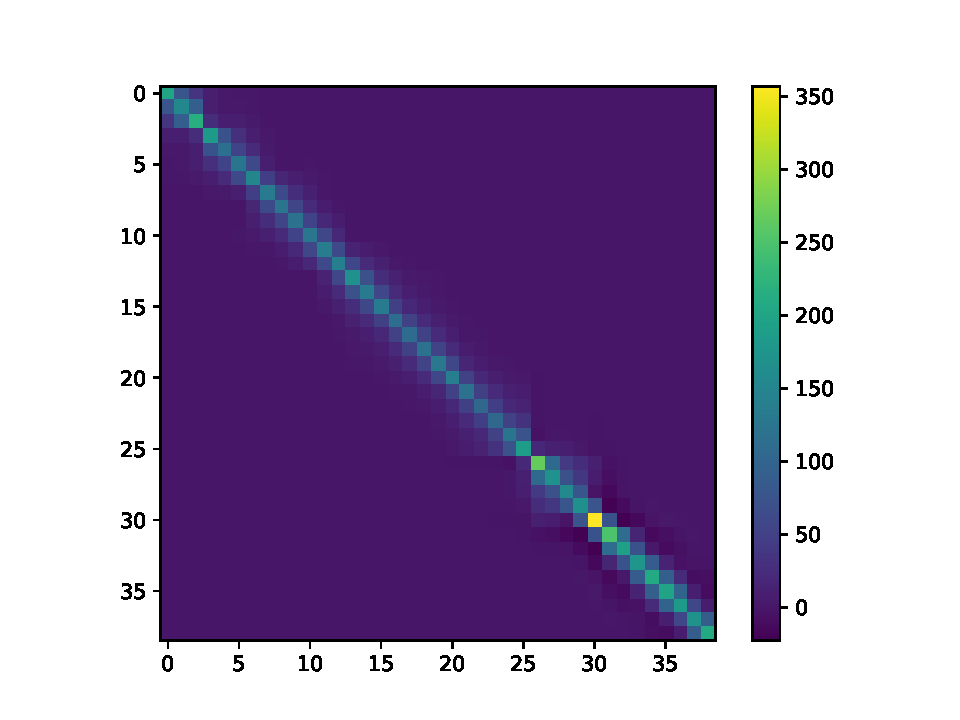
\includegraphics[width=0.7\textwidth]{images/hessian.pdf}
    \caption{Pasovna struktura Hessove matrike za $n=39$ segmentov trajektorije.}
    \label{fig:hess_band}
\end{figure}



\section{Eksperimenti}
\label{sec:eksperimenti}

V tem poglavju predstavimo rezultate eksperimentov, ki smo jih izvedli za oceno učinkovitostin naše metode. Najprej predstavimo implementacijske podrobnosti in uporabljene knjižnice. Nato analiziramo konvergenco naše metode, ki jo primerjamo z dvema drugima metodama, in sicer z metodo, ki uporablja samo analitično izračunani gradient, in metodo trust-region, ki uporablja numerično izračunani gradient in Hessovo matriko. Poleg tega analiziramo hitrost naše metode in njeno odvisnost od števila segmentov trajektorije. Na koncu proučimo pasovno strukturo Hessove matrike, kjer nas zanima kvaliteta algoritma glede na število pasov Hessove matrike, ki jih upoštevamo pri optimizaciji.

\subsection{Implementacija in uporaba zunanjih knjižnic}
Naša metoda je implementirana v programskem jeziku Python in je dostopna na povezavi \href{https://github.com/maticpokorn/trajectory_optimization}{\texttt{github.com/maticpokorn/trajectory\_optimization}}. V implementaciji se često zanašamo na operacije z redkimi matrikami za doseganje višje hitrosti in zato uprabljamo modul \texttt{scipy.sparse} knjižnice SciPy \cite{2020SciPy-NMeth}. Konkretno se poslužujemo metode SuperLU za faktorizacijo matrike v enačbi~\eqref{eq:kkt_matrix} \cite{superlu1997superlu}. Za reševanje QP uporabljamo knjižnico OSQP \cite{osqp}. Implemetacijo naše metode sta omogočili še knjižnici NumPy \cite{harris2020array} in Matplotlib \cite{Hunter:2007}.

\paragraph{Primer uporabe}
Tukaj prikažemo preprost primer uporabe naše metode \newline v Python-u. Spodaj je prikazana koda, kjer definiramo problem z $11$ vmesnimi točkami in skupnim časom trajektorije $T=10$. Nato pokličemo metodo, ki implementira algoritem~\ref{alg:newton}. V vrstici \texttt{solver = ...} določimo stopnjo polinoma, kateri odvod želimo optimizirati, stopnjo gladkosti trajektorije in dimenzionalnost prostora, v katerem se nahajajo točke.

\begin{verbatim}
from solver import NoTimestampSolver

solver = NoTimestampSolver(d=9, r=4, q=4, dimensions=3)

waypoints = [[0, 0, 0], [8, 4, 0], [2, 10, 0], [12, 14, 0], 
            [8, 22, 0], [3, 20, 0], [0, 25, 0], [-8, 20, 0], 
            [-4, 12, 0], [0, 8, 0], [4, 4, 0], [0, 0, 0]]

T = 10

result = solver.solve_backtracking_line_search(waypoints, T)
\end{verbatim}

Vizualizacija dobljene trajektorije je prikazana na sliki~\ref{fig:iterations_viz}, kjer so vidni tudi rezultati vmesnih iteracij optimizacije.
\begin{figure}
    \centering
    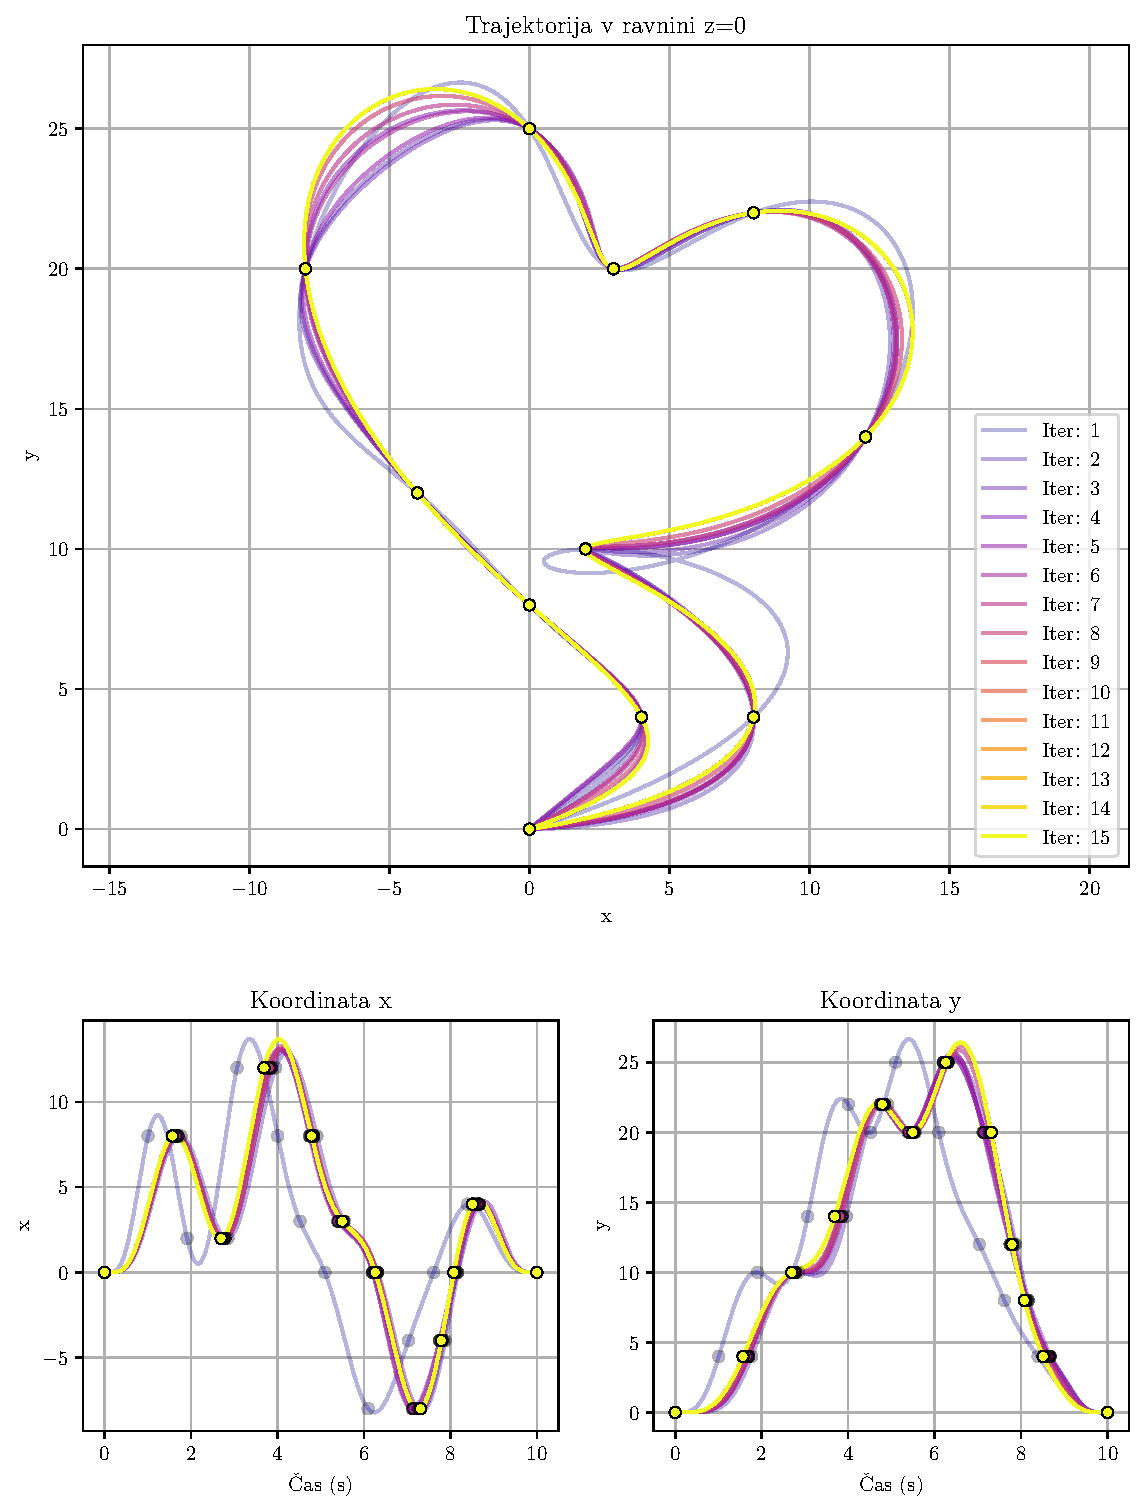
\includegraphics[width=0.99\textwidth]{images/iterations_viz.pdf}
    \caption{Vizualizacija konvergence na primeru. Na zgornjem grafu je prikazana trajektorija in vmesne točke v ravnini $z=0$ v različnih iteracijah optimizacije. Algoritem na vsakem koraku reši \ac{QP}, ki je parametriziran s časovnim vektorjem $\tvec$. Na spodnjih grafih je prikazana trajektorija po komponentah $x$ in $y$ v odvisnosti od časa, kjer pike označujejo čas in mesto, ko trajektorija prečka vmesno točko.}
    \label{fig:iterations_viz}
\end{figure}


\subsection{Konvergenca}
\label{sec:convergence}

V tem podpoglavju predstavimo rezultate ekseperimentov, s katerimi pokažemo primerjavo konvergence naše metode. Izmerimo konvergenco treh metod:
\begin{enumerate}
    \item Newtonova metoda, ki uporablja analitično izračunani gradient in Hessovo matriko, kot je opisano v algoritmu~\ref{alg:newton}.
    \item Metoda gradientnega spusta, ki uporablja samo analitično izračunani gradient, ki ga projiciramo na hiperravnino $\mathbf{1}^\top \mathbf{t} = T$.
    \item Dve metodi trust-constr (TC) iz paketa SciPy, ki uporabljata numerično oz. analitično izračunani gradient in Hessovo matriko ter metodo območja zaupanja \cite{conn2000trust}, ki dopušča linearne omejitve.
\end{enumerate}

Za eksperimente uporabimo naključno generirane probleme, ki jih definiramo na dva načina:
\begin{itemize}
    \item \textbf{Naključne točke:} Za vsak problem naključno generiramo $n$ točk znotraj kocke $[0, 1]^3$.
    \item \textbf{Naključna premica:} Za vsak problem naključno generiramo $n$ točk tako, da so koordinate $i$-te točke naključno izbrane znotraj kocke $[i-1, i]\times[0, 1]\times[0, 1]$. Torej, točke si v grobem sledijo po premici od $[0, 0, 0]$ do $[n-1, 0, 0]$.
\end{itemize}
    
Metodo poženemo tudi na različnem številu točk, in namreč si izberemo primere s $5$, $10$, $20$, $30$ in $40$ točkami.

Začetna točka $\tvec_0$ je v vseh primerih izbrana na sledeči način:
\begin{equation}
    t_{0i} = \frac{\|P_{i+1} - P_i\|}{\sum_{j=0}^{n-1} \|P_{j+1} - P_j\|} n
\end{equation},
torej čas segmenta je proporcionalen glede na evklidsko razdaljo med končnima točkama segmenta. Skupen čas trajektorije $T$ je nastavljen na $n$.

 Rezultati so prikazani na slikah~\ref{fig:convergence_random} in~\ref{fig:convergence_random_and_line}. Na grafih je na x osi število iteracij optimizacije, na y osi pa povprečna izboljšava vrednosti cenovne funkcije $F(\tvec_i)$ glede na začetno vrednost $F(\tvec_0)$, izračunana s formulo $y_i = 1 - \frac{F(\tvec_i)}{F(\tvec_0)}$. Vsi rezultati pokažejo, da Newtonova metoda konvergira hitreje kot metoda, ki uporablja samo gradient in metoda trust-region, kar potrjuje učinkovitost naše metode. Poleg tega lahko opazimo, da se hitrost konvergence zmanjšuje z večjim številom segmentov trajektorije in Newtonova metoda večinoma  izgubi prednost pred gradientnim spustom. Analitični in numerični TC sta večinoma slabša od ostalih dveh metod, čeprav analitčni TC skonvergira k malo boljši rešitvi kot gradientni spust. V vseh primerih pa tudi velja, da Newtonova metoda konvergira k boljši rešitvi kot gradientni spust, vendar pa je ta razlika v končni vrednosti cenovne funkcije zelo majhna in v praksi ne bi bila opazna. Opazimo lahko, da pri prvem naboru naključnih primerov analitični TC konvergira k rešitvi bistveno hitreje kot numerični TC, kar je verjetno pokazatelj nenatančnosti numerične ocene odvodov, ki jih numerični TC uporablja. Pri drugem naboru pa se izkaže, da je numerični TC v začetnih iteracijah boljši kot analitični TC, kar bi lahko bila posledica tega, da $F$ pri vrednostih $\tvec$ v začetnih iteracijah z večjo verjetnostjo ni konveksna; v vseh primerih namreč analitični TC skonvergira k boljši rešitvi kot numerični TC.



\begin{figure}
    \centering
    % To use in your document:
% \begin{figure}
%     \centering
%     % To use in your document:
% \begin{figure}
%     \centering
%     % To use in your document:
% \begin{figure}
%     \centering
%     \input{tikz/convergence_analysis_random.tex}
%     \caption{Analiza konvergence z naključnimi začetnimi točkami}
%     \label{fig:convergence_random}
% \end{figure}
\def\yrange{0.15}
\def\ymina{0.4}
\def\yminb{0.55}
\def\yminc{0.55}
\def\ymind{0.55}
\def\ymine{0.55}
\def\width{0.49\textwidth}
\def\plotwidth{0.7\textwidth}
\def\gridstyle{dashed}

\begin{subfigure}[b]{\width}
    \centering
    \begin{tikzpicture}
    \begin{axis}[
        xlabel={Iteracija},
        ylabel={Vrednost $F$},
        xmin=0, xmax=20,
        ymin=\ymina, ymax={\ymina+\yrange},
        legend pos=south east,
        xmajorgrids=true,
        ymajorgrids=true,
        minor tick num=1,
        grid=both,
        grid style=\gridstyle,
        width=\plotwidth,
        height=5cm,
        scale only axis,
    ]
    \addplot[color=blue, thick] table [x=iteration, y expr=\thisrow{newton_mean}, col sep=comma] {data/convergence_results_random_5.csv};
    \addplot[color=red, thick] table [x=iteration, y expr=\thisrow{gradient_mean}, col sep=comma] {data/convergence_results_random_5.csv};
    \addplot[color=black!60!green, thick] table [x=iteration, y expr=\thisrow{trust-constr_mean}, col sep=comma] {data/convergence_results_random_5.csv};
    \legend{Newton, Gradient, Trust-constr}
    \end{axis}
    \end{tikzpicture}
    \caption{$n=5$ točk}
\end{subfigure}
\hfill
\begin{subfigure}[b]{\width}
    \centering
    \begin{tikzpicture}
    \begin{axis}[
        xlabel={Iteracija},
        ylabel={Vrednost $F$},
        xmin=0, xmax=20,
        ymin=\yminb, ymax={\yminb+\yrange},
        legend pos=south east,
        xmajorgrids=true,
        ymajorgrids=true,
        minor tick num=1,
        grid=both,
        grid style=\gridstyle,
        width=\plotwidth,
        height=5cm,
        scale only axis,
    ]
    \addplot[color=blue, thick] table [x=iteration, y expr=\thisrow{newton_mean}, col sep=comma] {data/convergence_results_random_10.csv};
    \addplot[color=red, thick] table [x=iteration, y expr=\thisrow{gradient_mean}, col sep=comma] {data/convergence_results_random_10.csv};
    \addplot[color=black!60!green, thick] table [x=iteration, y expr=\thisrow{trust-constr_mean}, col sep=comma] {data/convergence_results_random_10.csv};
    \legend{Newton, Gradient, Trust-constr}
    \end{axis}
    \end{tikzpicture}
    \caption{$n=10$ točk}
\end{subfigure}

\vspace{0.5cm}

\begin{subfigure}[b]{\width}
    \centering
    \begin{tikzpicture}
    \begin{axis}[
        xlabel={Iteracija},
        ylabel={Vrednost $F$},
        xmin=0, xmax=20,
        ymin=\yminc, ymax={\yminc+\yrange},
        legend pos=south east,
        xmajorgrids=true,
        ymajorgrids=true,
        minor tick num=1,
        grid=both,
        grid style=\gridstyle,
        width=\plotwidth,
        height=5cm,
        scale only axis,
    ]
    \addplot[color=blue, thick] table [x=iteration, y expr=\thisrow{newton_mean}, col sep=comma] {data/convergence_results_random_20.csv};
    \addplot[color=red, thick] table [x=iteration, y expr=\thisrow{gradient_mean}, col sep=comma] {data/convergence_results_random_20.csv};
    \addplot[color=black!60!green, thick] table [x=iteration, y expr=\thisrow{trust-constr_mean}, col sep=comma] {data/convergence_results_random_20.csv};
    \legend{Newton, Gradient, Trust-constr}
    \end{axis}
    \end{tikzpicture}
    \caption{$n=20$ točk}
\end{subfigure}
\hfill
\begin{subfigure}[b]{\width}
    \centering
    \begin{tikzpicture}
    \begin{axis}[
        xlabel={Iteracija},
        ylabel={Vrednost $F$},
        xmin=0, xmax=20,
        ymin=\ymind, ymax={\ymind+\yrange},
        legend pos=south east,
        xmajorgrids=true,
        ymajorgrids=true,
        minor tick num=1,
        grid=both,
        grid style=\gridstyle,
        width=\plotwidth,
        height=5cm,
        scale only axis,
    ]
    \addplot[color=blue, thick] table [x=iteration, y expr=\thisrow{newton_mean}, col sep=comma] {data/convergence_results_random_30.csv};
    \addplot[color=red, thick] table [x=iteration, y expr=\thisrow{gradient_mean}, col sep=comma] {data/convergence_results_random_30.csv};
    \addplot[color=black!60!green, thick] table [x=iteration, y expr=\thisrow{trust-constr_mean}, col sep=comma] {data/convergence_results_random_30.csv};
    \legend{Newton, Gradient, Trust-constr}
    \end{axis}
    \end{tikzpicture}
    \caption{$n=30$ točk}
\end{subfigure}

\vspace{0.5cm}

\begin{subfigure}[b]{\width}
    \centering
    \begin{tikzpicture}
    \begin{axis}[
        xlabel={Iteracija},
        ylabel={Vrednost $F$},
        xmin=0, xmax=20,
        ymin=\ymine, ymax={\ymine+\yrange},
        legend pos=south east,
        xmajorgrids=true,
        ymajorgrids=true,
        minor tick num=1,
        grid=both,
        grid style=\gridstyle,
        width=\plotwidth,
        height=5cm,
        scale only axis,
    ]
    \addplot[color=blue, thick] table [x=iteration, y expr=\thisrow{newton_mean}, col sep=comma] {data/convergence_results_random_40.csv};
    \addplot[color=red, thick] table [x=iteration, y expr=\thisrow{gradient_mean}, col sep=comma] {data/convergence_results_random_40.csv};
    \addplot[color=black!60!green, thick] table [x=iteration, y expr=\thisrow{trust-constr_mean}, col sep=comma] {data/convergence_results_random_40.csv};
    \legend{Newton, Gradient, Trust-constr}
    \end{axis}
    \end{tikzpicture}
    \caption{$n=40$ točk}
\end{subfigure}

%     \caption{Analiza konvergence z naključnimi začetnimi točkami}
%     \label{fig:convergence_random}
% \end{figure}
\def\yrange{0.15}
\def\ymina{0.4}
\def\yminb{0.55}
\def\yminc{0.55}
\def\ymind{0.55}
\def\ymine{0.55}
\def\width{0.49\textwidth}
\def\plotwidth{0.7\textwidth}
\def\gridstyle{dashed}

\begin{subfigure}[b]{\width}
    \centering
    \begin{tikzpicture}
    \begin{axis}[
        xlabel={Iteracija},
        ylabel={Vrednost $F$},
        xmin=0, xmax=20,
        ymin=\ymina, ymax={\ymina+\yrange},
        legend pos=south east,
        xmajorgrids=true,
        ymajorgrids=true,
        minor tick num=1,
        grid=both,
        grid style=\gridstyle,
        width=\plotwidth,
        height=5cm,
        scale only axis,
    ]
    \addplot[color=blue, thick] table [x=iteration, y expr=\thisrow{newton_mean}, col sep=comma] {data/convergence_results_random_5.csv};
    \addplot[color=red, thick] table [x=iteration, y expr=\thisrow{gradient_mean}, col sep=comma] {data/convergence_results_random_5.csv};
    \addplot[color=black!60!green, thick] table [x=iteration, y expr=\thisrow{trust-constr_mean}, col sep=comma] {data/convergence_results_random_5.csv};
    \legend{Newton, Gradient, Trust-constr}
    \end{axis}
    \end{tikzpicture}
    \caption{$n=5$ točk}
\end{subfigure}
\hfill
\begin{subfigure}[b]{\width}
    \centering
    \begin{tikzpicture}
    \begin{axis}[
        xlabel={Iteracija},
        ylabel={Vrednost $F$},
        xmin=0, xmax=20,
        ymin=\yminb, ymax={\yminb+\yrange},
        legend pos=south east,
        xmajorgrids=true,
        ymajorgrids=true,
        minor tick num=1,
        grid=both,
        grid style=\gridstyle,
        width=\plotwidth,
        height=5cm,
        scale only axis,
    ]
    \addplot[color=blue, thick] table [x=iteration, y expr=\thisrow{newton_mean}, col sep=comma] {data/convergence_results_random_10.csv};
    \addplot[color=red, thick] table [x=iteration, y expr=\thisrow{gradient_mean}, col sep=comma] {data/convergence_results_random_10.csv};
    \addplot[color=black!60!green, thick] table [x=iteration, y expr=\thisrow{trust-constr_mean}, col sep=comma] {data/convergence_results_random_10.csv};
    \legend{Newton, Gradient, Trust-constr}
    \end{axis}
    \end{tikzpicture}
    \caption{$n=10$ točk}
\end{subfigure}

\vspace{0.5cm}

\begin{subfigure}[b]{\width}
    \centering
    \begin{tikzpicture}
    \begin{axis}[
        xlabel={Iteracija},
        ylabel={Vrednost $F$},
        xmin=0, xmax=20,
        ymin=\yminc, ymax={\yminc+\yrange},
        legend pos=south east,
        xmajorgrids=true,
        ymajorgrids=true,
        minor tick num=1,
        grid=both,
        grid style=\gridstyle,
        width=\plotwidth,
        height=5cm,
        scale only axis,
    ]
    \addplot[color=blue, thick] table [x=iteration, y expr=\thisrow{newton_mean}, col sep=comma] {data/convergence_results_random_20.csv};
    \addplot[color=red, thick] table [x=iteration, y expr=\thisrow{gradient_mean}, col sep=comma] {data/convergence_results_random_20.csv};
    \addplot[color=black!60!green, thick] table [x=iteration, y expr=\thisrow{trust-constr_mean}, col sep=comma] {data/convergence_results_random_20.csv};
    \legend{Newton, Gradient, Trust-constr}
    \end{axis}
    \end{tikzpicture}
    \caption{$n=20$ točk}
\end{subfigure}
\hfill
\begin{subfigure}[b]{\width}
    \centering
    \begin{tikzpicture}
    \begin{axis}[
        xlabel={Iteracija},
        ylabel={Vrednost $F$},
        xmin=0, xmax=20,
        ymin=\ymind, ymax={\ymind+\yrange},
        legend pos=south east,
        xmajorgrids=true,
        ymajorgrids=true,
        minor tick num=1,
        grid=both,
        grid style=\gridstyle,
        width=\plotwidth,
        height=5cm,
        scale only axis,
    ]
    \addplot[color=blue, thick] table [x=iteration, y expr=\thisrow{newton_mean}, col sep=comma] {data/convergence_results_random_30.csv};
    \addplot[color=red, thick] table [x=iteration, y expr=\thisrow{gradient_mean}, col sep=comma] {data/convergence_results_random_30.csv};
    \addplot[color=black!60!green, thick] table [x=iteration, y expr=\thisrow{trust-constr_mean}, col sep=comma] {data/convergence_results_random_30.csv};
    \legend{Newton, Gradient, Trust-constr}
    \end{axis}
    \end{tikzpicture}
    \caption{$n=30$ točk}
\end{subfigure}

\vspace{0.5cm}

\begin{subfigure}[b]{\width}
    \centering
    \begin{tikzpicture}
    \begin{axis}[
        xlabel={Iteracija},
        ylabel={Vrednost $F$},
        xmin=0, xmax=20,
        ymin=\ymine, ymax={\ymine+\yrange},
        legend pos=south east,
        xmajorgrids=true,
        ymajorgrids=true,
        minor tick num=1,
        grid=both,
        grid style=\gridstyle,
        width=\plotwidth,
        height=5cm,
        scale only axis,
    ]
    \addplot[color=blue, thick] table [x=iteration, y expr=\thisrow{newton_mean}, col sep=comma] {data/convergence_results_random_40.csv};
    \addplot[color=red, thick] table [x=iteration, y expr=\thisrow{gradient_mean}, col sep=comma] {data/convergence_results_random_40.csv};
    \addplot[color=black!60!green, thick] table [x=iteration, y expr=\thisrow{trust-constr_mean}, col sep=comma] {data/convergence_results_random_40.csv};
    \legend{Newton, Gradient, Trust-constr}
    \end{axis}
    \end{tikzpicture}
    \caption{$n=40$ točk}
\end{subfigure}

%     \caption{Analiza konvergence z naključnimi začetnimi točkami}
%     \label{fig:convergence_random}
% \end{figure}
\def\yrange{0.15}
\def\ymina{0.4}
\def\yminb{0.55}
\def\yminc{0.55}
\def\ymind{0.55}
\def\ymine{0.55}
\def\width{0.49\textwidth}
\def\plotwidth{0.7\textwidth}
\def\gridstyle{dashed}

\begin{subfigure}[b]{\width}
    \centering
    \begin{tikzpicture}
    \begin{axis}[
        xlabel={Iteracija},
        ylabel={Vrednost $F$},
        xmin=0, xmax=20,
        ymin=\ymina, ymax={\ymina+\yrange},
        legend pos=south east,
        xmajorgrids=true,
        ymajorgrids=true,
        minor tick num=1,
        grid=both,
        grid style=\gridstyle,
        width=\plotwidth,
        height=5cm,
        scale only axis,
    ]
    \addplot[color=blue, thick] table [x=iteration, y expr=\thisrow{newton_mean}, col sep=comma] {data/convergence_results_random_5.csv};
    \addplot[color=red, thick] table [x=iteration, y expr=\thisrow{gradient_mean}, col sep=comma] {data/convergence_results_random_5.csv};
    \addplot[color=black!60!green, thick] table [x=iteration, y expr=\thisrow{trust-constr_mean}, col sep=comma] {data/convergence_results_random_5.csv};
    \legend{Newton, Gradient, Trust-constr}
    \end{axis}
    \end{tikzpicture}
    \caption{$n=5$ točk}
\end{subfigure}
\hfill
\begin{subfigure}[b]{\width}
    \centering
    \begin{tikzpicture}
    \begin{axis}[
        xlabel={Iteracija},
        ylabel={Vrednost $F$},
        xmin=0, xmax=20,
        ymin=\yminb, ymax={\yminb+\yrange},
        legend pos=south east,
        xmajorgrids=true,
        ymajorgrids=true,
        minor tick num=1,
        grid=both,
        grid style=\gridstyle,
        width=\plotwidth,
        height=5cm,
        scale only axis,
    ]
    \addplot[color=blue, thick] table [x=iteration, y expr=\thisrow{newton_mean}, col sep=comma] {data/convergence_results_random_10.csv};
    \addplot[color=red, thick] table [x=iteration, y expr=\thisrow{gradient_mean}, col sep=comma] {data/convergence_results_random_10.csv};
    \addplot[color=black!60!green, thick] table [x=iteration, y expr=\thisrow{trust-constr_mean}, col sep=comma] {data/convergence_results_random_10.csv};
    \legend{Newton, Gradient, Trust-constr}
    \end{axis}
    \end{tikzpicture}
    \caption{$n=10$ točk}
\end{subfigure}

\vspace{0.5cm}

\begin{subfigure}[b]{\width}
    \centering
    \begin{tikzpicture}
    \begin{axis}[
        xlabel={Iteracija},
        ylabel={Vrednost $F$},
        xmin=0, xmax=20,
        ymin=\yminc, ymax={\yminc+\yrange},
        legend pos=south east,
        xmajorgrids=true,
        ymajorgrids=true,
        minor tick num=1,
        grid=both,
        grid style=\gridstyle,
        width=\plotwidth,
        height=5cm,
        scale only axis,
    ]
    \addplot[color=blue, thick] table [x=iteration, y expr=\thisrow{newton_mean}, col sep=comma] {data/convergence_results_random_20.csv};
    \addplot[color=red, thick] table [x=iteration, y expr=\thisrow{gradient_mean}, col sep=comma] {data/convergence_results_random_20.csv};
    \addplot[color=black!60!green, thick] table [x=iteration, y expr=\thisrow{trust-constr_mean}, col sep=comma] {data/convergence_results_random_20.csv};
    \legend{Newton, Gradient, Trust-constr}
    \end{axis}
    \end{tikzpicture}
    \caption{$n=20$ točk}
\end{subfigure}
\hfill
\begin{subfigure}[b]{\width}
    \centering
    \begin{tikzpicture}
    \begin{axis}[
        xlabel={Iteracija},
        ylabel={Vrednost $F$},
        xmin=0, xmax=20,
        ymin=\ymind, ymax={\ymind+\yrange},
        legend pos=south east,
        xmajorgrids=true,
        ymajorgrids=true,
        minor tick num=1,
        grid=both,
        grid style=\gridstyle,
        width=\plotwidth,
        height=5cm,
        scale only axis,
    ]
    \addplot[color=blue, thick] table [x=iteration, y expr=\thisrow{newton_mean}, col sep=comma] {data/convergence_results_random_30.csv};
    \addplot[color=red, thick] table [x=iteration, y expr=\thisrow{gradient_mean}, col sep=comma] {data/convergence_results_random_30.csv};
    \addplot[color=black!60!green, thick] table [x=iteration, y expr=\thisrow{trust-constr_mean}, col sep=comma] {data/convergence_results_random_30.csv};
    \legend{Newton, Gradient, Trust-constr}
    \end{axis}
    \end{tikzpicture}
    \caption{$n=30$ točk}
\end{subfigure}

\vspace{0.5cm}

\begin{subfigure}[b]{\width}
    \centering
    \begin{tikzpicture}
    \begin{axis}[
        xlabel={Iteracija},
        ylabel={Vrednost $F$},
        xmin=0, xmax=20,
        ymin=\ymine, ymax={\ymine+\yrange},
        legend pos=south east,
        xmajorgrids=true,
        ymajorgrids=true,
        minor tick num=1,
        grid=both,
        grid style=\gridstyle,
        width=\plotwidth,
        height=5cm,
        scale only axis,
    ]
    \addplot[color=blue, thick] table [x=iteration, y expr=\thisrow{newton_mean}, col sep=comma] {data/convergence_results_random_40.csv};
    \addplot[color=red, thick] table [x=iteration, y expr=\thisrow{gradient_mean}, col sep=comma] {data/convergence_results_random_40.csv};
    \addplot[color=black!60!green, thick] table [x=iteration, y expr=\thisrow{trust-constr_mean}, col sep=comma] {data/convergence_results_random_40.csv};
    \legend{Newton, Gradient, Trust-constr}
    \end{axis}
    \end{tikzpicture}
    \caption{$n=40$ točk}
\end{subfigure}

    \caption{Konvergenca z naključnimi začetnimi točkami. V vseh primerih Newtonova metoda konvergira hitreje kot metoda z gradientnim spustom.}
    \label{fig:convergence_random}
\end{figure}

\begin{figure}
    \centering
    % To use in your document:
% \begin{figure}
%     \centering
%     % To use in your document:
% \begin{figure}
%     \centering
%     % To use in your document:
% \begin{figure}
%     \centering
%     \input{tikz/convergence_analysis_random_and_line.tex}
%     \caption{Analiza konvergence z naključnimi točkami in premicami}
%     \label{fig:convergence_random_and_line}
% \end{figure}
\def\yrange{0.15}
\def\ymina{0.55}
\def\yminb{0.70}
\def\yminc{0.70}
\def\ymind{0.70}
\def\ymine{0.70}
\def\width{0.49\textwidth}
\def\plotwidth{0.7\textwidth}
\def\gridstyle{dashed}

\begin{subfigure}[b]{\width}
    \centering
    \begin{tikzpicture}
    \begin{axis}[
        xlabel={Iteracija},
        ylabel={Vrednost $F$},
        xmin=0, xmax=20,
        ymin=\ymina, ymax={\ymina+\yrange},
        legend pos=south east,
        xmajorgrids=true,
        ymajorgrids=true,
        minor tick num=1,
        grid=both,
        grid style=\gridstyle,
        width=\plotwidth,
        height=5cm,
        scale only axis,
    ]
    \addplot[color=blue, thick] table [x=iteration, y expr=\thisrow{newton_mean}, col sep=comma] {data/convergence_results_random_and_line_5.csv};
    \addplot[color=red, thick] table [x=iteration, y expr=\thisrow{gradient_mean}, col sep=comma] {data/convergence_results_random_and_line_5.csv};
    \addplot[color=black!60!green, thick] table [x=iteration, y expr=\thisrow{trust-constr_mean}, col sep=comma] {data/convergence_results_random_and_line_5.csv};
    \legend{Newton, Gradient, Trust-constr}
    \end{axis}
    \end{tikzpicture}
    \caption{$n=5$ točk}
\end{subfigure}
\hfill
\begin{subfigure}[b]{\width}
    \centering
    \begin{tikzpicture}
    \begin{axis}[
        xlabel={Iteracija},
        ylabel={Vrednost $F$},
        xmin=0, xmax=20,
        ymin=\yminb, ymax={\yminb+\yrange},
        legend pos=south east,
        xmajorgrids=true,
        ymajorgrids=true,
        minor tick num=1,
        grid=both,
        grid style=\gridstyle,
        width=\plotwidth,
        height=5cm,
        scale only axis,
    ]
    \addplot[color=blue, thick] table [x=iteration, y expr=\thisrow{newton_mean}, col sep=comma] {data/convergence_results_random_and_line_10.csv};
    \addplot[color=red, thick] table [x=iteration, y expr=\thisrow{gradient_mean}, col sep=comma] {data/convergence_results_random_and_line_10.csv};
    \addplot[color=black!60!green, thick] table [x=iteration, y expr=\thisrow{trust-constr_mean}, col sep=comma] {data/convergence_results_random_and_line_10.csv};
    \legend{Newton, Gradient, Trust-constr}
    \end{axis}
    \end{tikzpicture}
    \caption{$n=10$ točk}
\end{subfigure}

\vspace{0.5cm}

\begin{subfigure}[b]{\width}
    \centering
    \begin{tikzpicture}
    \begin{axis}[
        xlabel={Iteracija},
        ylabel={Vrednost $F$},
        xmin=0, xmax=20,
        ymin=\yminc, ymax={\yminc+\yrange},
        legend pos=south east,
        xmajorgrids=true,
        ymajorgrids=true,
        minor tick num=1,
        grid=both,
        grid style=\gridstyle,
        width=\plotwidth,
        height=5cm,
        scale only axis,
    ]
    \addplot[color=blue, thick] table [x=iteration, y expr=\thisrow{newton_mean}, col sep=comma] {data/convergence_results_random_and_line_20.csv};
    \addplot[color=red, thick] table [x=iteration, y expr=\thisrow{gradient_mean}, col sep=comma] {data/convergence_results_random_and_line_20.csv};
    \addplot[color=black!60!green, thick] table [x=iteration, y expr=\thisrow{trust-constr_mean}, col sep=comma] {data/convergence_results_random_and_line_20.csv};
    \legend{Newton, Gradient, Trust-constr}
    \end{axis}
    \end{tikzpicture}
    \caption{$n=20$ točk}
\end{subfigure}
\hfill
\begin{subfigure}[b]{\width}
    \centering
    \begin{tikzpicture}
    \begin{axis}[
        xlabel={Iteracija},
        ylabel={Vrednost $F$},
        xmin=0, xmax=20,
        ymin=\ymind, ymax={\ymind+\yrange},
        legend pos=south east,
        xmajorgrids=true,
        ymajorgrids=true,
        minor tick num=1,
        grid=both,
        grid style=\gridstyle,
        width=\plotwidth,
        height=5cm,
        scale only axis,
    ]
    \addplot[color=blue, thick] table [x=iteration, y expr=\thisrow{newton_mean}, col sep=comma] {data/convergence_results_random_and_line_30.csv};
    \addplot[color=red, thick] table [x=iteration, y expr=\thisrow{gradient_mean}, col sep=comma] {data/convergence_results_random_and_line_30.csv};
    \addplot[color=black!60!green, thick] table [x=iteration, y expr=\thisrow{trust-constr_mean}, col sep=comma] {data/convergence_results_random_and_line_30.csv};
    \legend{Newton, Gradient, Trust-constr}
    \end{axis}
    \end{tikzpicture}
    \caption{$n=30$ točk}
\end{subfigure}

\vspace{0.5cm}

\begin{subfigure}[b]{\width}
    \centering
    \begin{tikzpicture}
    \begin{axis}[
        xlabel={Iteracija},
        ylabel={Vrednost $F$},
        xmin=0, xmax=20,
        ymin=\ymine, ymax={\ymine+\yrange},
        legend pos=south east,
        xmajorgrids=true,
        ymajorgrids=true,
        minor tick num=1,
        grid=both,
        grid style=\gridstyle,
        width=\plotwidth,
        height=5cm,
        scale only axis,
    ]
    \addplot[color=blue, thick] table [x=iteration, y expr=\thisrow{newton_mean}, col sep=comma] {data/convergence_results_random_and_line_40.csv};
    \addplot[color=red, thick] table [x=iteration, y expr=\thisrow{gradient_mean}, col sep=comma] {data/convergence_results_random_and_line_40.csv};
    \addplot[color=black!60!green, thick] table [x=iteration, y expr=\thisrow{trust-constr_mean}, col sep=comma] {data/convergence_results_random_and_line_40.csv};
    \legend{Newton, Gradient, Trust-constr}
    \end{axis}
    \end{tikzpicture}
    \caption{$n=40$ točk}
\end{subfigure}

%     \caption{Analiza konvergence z naključnimi točkami in premicami}
%     \label{fig:convergence_random_and_line}
% \end{figure}
\def\yrange{0.15}
\def\ymina{0.55}
\def\yminb{0.70}
\def\yminc{0.70}
\def\ymind{0.70}
\def\ymine{0.70}
\def\width{0.49\textwidth}
\def\plotwidth{0.7\textwidth}
\def\gridstyle{dashed}

\begin{subfigure}[b]{\width}
    \centering
    \begin{tikzpicture}
    \begin{axis}[
        xlabel={Iteracija},
        ylabel={Vrednost $F$},
        xmin=0, xmax=20,
        ymin=\ymina, ymax={\ymina+\yrange},
        legend pos=south east,
        xmajorgrids=true,
        ymajorgrids=true,
        minor tick num=1,
        grid=both,
        grid style=\gridstyle,
        width=\plotwidth,
        height=5cm,
        scale only axis,
    ]
    \addplot[color=blue, thick] table [x=iteration, y expr=\thisrow{newton_mean}, col sep=comma] {data/convergence_results_random_and_line_5.csv};
    \addplot[color=red, thick] table [x=iteration, y expr=\thisrow{gradient_mean}, col sep=comma] {data/convergence_results_random_and_line_5.csv};
    \addplot[color=black!60!green, thick] table [x=iteration, y expr=\thisrow{trust-constr_mean}, col sep=comma] {data/convergence_results_random_and_line_5.csv};
    \legend{Newton, Gradient, Trust-constr}
    \end{axis}
    \end{tikzpicture}
    \caption{$n=5$ točk}
\end{subfigure}
\hfill
\begin{subfigure}[b]{\width}
    \centering
    \begin{tikzpicture}
    \begin{axis}[
        xlabel={Iteracija},
        ylabel={Vrednost $F$},
        xmin=0, xmax=20,
        ymin=\yminb, ymax={\yminb+\yrange},
        legend pos=south east,
        xmajorgrids=true,
        ymajorgrids=true,
        minor tick num=1,
        grid=both,
        grid style=\gridstyle,
        width=\plotwidth,
        height=5cm,
        scale only axis,
    ]
    \addplot[color=blue, thick] table [x=iteration, y expr=\thisrow{newton_mean}, col sep=comma] {data/convergence_results_random_and_line_10.csv};
    \addplot[color=red, thick] table [x=iteration, y expr=\thisrow{gradient_mean}, col sep=comma] {data/convergence_results_random_and_line_10.csv};
    \addplot[color=black!60!green, thick] table [x=iteration, y expr=\thisrow{trust-constr_mean}, col sep=comma] {data/convergence_results_random_and_line_10.csv};
    \legend{Newton, Gradient, Trust-constr}
    \end{axis}
    \end{tikzpicture}
    \caption{$n=10$ točk}
\end{subfigure}

\vspace{0.5cm}

\begin{subfigure}[b]{\width}
    \centering
    \begin{tikzpicture}
    \begin{axis}[
        xlabel={Iteracija},
        ylabel={Vrednost $F$},
        xmin=0, xmax=20,
        ymin=\yminc, ymax={\yminc+\yrange},
        legend pos=south east,
        xmajorgrids=true,
        ymajorgrids=true,
        minor tick num=1,
        grid=both,
        grid style=\gridstyle,
        width=\plotwidth,
        height=5cm,
        scale only axis,
    ]
    \addplot[color=blue, thick] table [x=iteration, y expr=\thisrow{newton_mean}, col sep=comma] {data/convergence_results_random_and_line_20.csv};
    \addplot[color=red, thick] table [x=iteration, y expr=\thisrow{gradient_mean}, col sep=comma] {data/convergence_results_random_and_line_20.csv};
    \addplot[color=black!60!green, thick] table [x=iteration, y expr=\thisrow{trust-constr_mean}, col sep=comma] {data/convergence_results_random_and_line_20.csv};
    \legend{Newton, Gradient, Trust-constr}
    \end{axis}
    \end{tikzpicture}
    \caption{$n=20$ točk}
\end{subfigure}
\hfill
\begin{subfigure}[b]{\width}
    \centering
    \begin{tikzpicture}
    \begin{axis}[
        xlabel={Iteracija},
        ylabel={Vrednost $F$},
        xmin=0, xmax=20,
        ymin=\ymind, ymax={\ymind+\yrange},
        legend pos=south east,
        xmajorgrids=true,
        ymajorgrids=true,
        minor tick num=1,
        grid=both,
        grid style=\gridstyle,
        width=\plotwidth,
        height=5cm,
        scale only axis,
    ]
    \addplot[color=blue, thick] table [x=iteration, y expr=\thisrow{newton_mean}, col sep=comma] {data/convergence_results_random_and_line_30.csv};
    \addplot[color=red, thick] table [x=iteration, y expr=\thisrow{gradient_mean}, col sep=comma] {data/convergence_results_random_and_line_30.csv};
    \addplot[color=black!60!green, thick] table [x=iteration, y expr=\thisrow{trust-constr_mean}, col sep=comma] {data/convergence_results_random_and_line_30.csv};
    \legend{Newton, Gradient, Trust-constr}
    \end{axis}
    \end{tikzpicture}
    \caption{$n=30$ točk}
\end{subfigure}

\vspace{0.5cm}

\begin{subfigure}[b]{\width}
    \centering
    \begin{tikzpicture}
    \begin{axis}[
        xlabel={Iteracija},
        ylabel={Vrednost $F$},
        xmin=0, xmax=20,
        ymin=\ymine, ymax={\ymine+\yrange},
        legend pos=south east,
        xmajorgrids=true,
        ymajorgrids=true,
        minor tick num=1,
        grid=both,
        grid style=\gridstyle,
        width=\plotwidth,
        height=5cm,
        scale only axis,
    ]
    \addplot[color=blue, thick] table [x=iteration, y expr=\thisrow{newton_mean}, col sep=comma] {data/convergence_results_random_and_line_40.csv};
    \addplot[color=red, thick] table [x=iteration, y expr=\thisrow{gradient_mean}, col sep=comma] {data/convergence_results_random_and_line_40.csv};
    \addplot[color=black!60!green, thick] table [x=iteration, y expr=\thisrow{trust-constr_mean}, col sep=comma] {data/convergence_results_random_and_line_40.csv};
    \legend{Newton, Gradient, Trust-constr}
    \end{axis}
    \end{tikzpicture}
    \caption{$n=40$ točk}
\end{subfigure}

%     \caption{Analiza konvergence z naključnimi točkami in premicami}
%     \label{fig:convergence_random_and_line}
% \end{figure}
\def\yrange{0.15}
\def\ymina{0.55}
\def\yminb{0.70}
\def\yminc{0.70}
\def\ymind{0.70}
\def\ymine{0.70}
\def\width{0.49\textwidth}
\def\plotwidth{0.7\textwidth}
\def\gridstyle{dashed}

\begin{subfigure}[b]{\width}
    \centering
    \begin{tikzpicture}
    \begin{axis}[
        xlabel={Iteracija},
        ylabel={Vrednost $F$},
        xmin=0, xmax=20,
        ymin=\ymina, ymax={\ymina+\yrange},
        legend pos=south east,
        xmajorgrids=true,
        ymajorgrids=true,
        minor tick num=1,
        grid=both,
        grid style=\gridstyle,
        width=\plotwidth,
        height=5cm,
        scale only axis,
    ]
    \addplot[color=blue, thick] table [x=iteration, y expr=\thisrow{newton_mean}, col sep=comma] {data/convergence_results_random_and_line_5.csv};
    \addplot[color=red, thick] table [x=iteration, y expr=\thisrow{gradient_mean}, col sep=comma] {data/convergence_results_random_and_line_5.csv};
    \addplot[color=black!60!green, thick] table [x=iteration, y expr=\thisrow{trust-constr_mean}, col sep=comma] {data/convergence_results_random_and_line_5.csv};
    \legend{Newton, Gradient, Trust-constr}
    \end{axis}
    \end{tikzpicture}
    \caption{$n=5$ točk}
\end{subfigure}
\hfill
\begin{subfigure}[b]{\width}
    \centering
    \begin{tikzpicture}
    \begin{axis}[
        xlabel={Iteracija},
        ylabel={Vrednost $F$},
        xmin=0, xmax=20,
        ymin=\yminb, ymax={\yminb+\yrange},
        legend pos=south east,
        xmajorgrids=true,
        ymajorgrids=true,
        minor tick num=1,
        grid=both,
        grid style=\gridstyle,
        width=\plotwidth,
        height=5cm,
        scale only axis,
    ]
    \addplot[color=blue, thick] table [x=iteration, y expr=\thisrow{newton_mean}, col sep=comma] {data/convergence_results_random_and_line_10.csv};
    \addplot[color=red, thick] table [x=iteration, y expr=\thisrow{gradient_mean}, col sep=comma] {data/convergence_results_random_and_line_10.csv};
    \addplot[color=black!60!green, thick] table [x=iteration, y expr=\thisrow{trust-constr_mean}, col sep=comma] {data/convergence_results_random_and_line_10.csv};
    \legend{Newton, Gradient, Trust-constr}
    \end{axis}
    \end{tikzpicture}
    \caption{$n=10$ točk}
\end{subfigure}

\vspace{0.5cm}

\begin{subfigure}[b]{\width}
    \centering
    \begin{tikzpicture}
    \begin{axis}[
        xlabel={Iteracija},
        ylabel={Vrednost $F$},
        xmin=0, xmax=20,
        ymin=\yminc, ymax={\yminc+\yrange},
        legend pos=south east,
        xmajorgrids=true,
        ymajorgrids=true,
        minor tick num=1,
        grid=both,
        grid style=\gridstyle,
        width=\plotwidth,
        height=5cm,
        scale only axis,
    ]
    \addplot[color=blue, thick] table [x=iteration, y expr=\thisrow{newton_mean}, col sep=comma] {data/convergence_results_random_and_line_20.csv};
    \addplot[color=red, thick] table [x=iteration, y expr=\thisrow{gradient_mean}, col sep=comma] {data/convergence_results_random_and_line_20.csv};
    \addplot[color=black!60!green, thick] table [x=iteration, y expr=\thisrow{trust-constr_mean}, col sep=comma] {data/convergence_results_random_and_line_20.csv};
    \legend{Newton, Gradient, Trust-constr}
    \end{axis}
    \end{tikzpicture}
    \caption{$n=20$ točk}
\end{subfigure}
\hfill
\begin{subfigure}[b]{\width}
    \centering
    \begin{tikzpicture}
    \begin{axis}[
        xlabel={Iteracija},
        ylabel={Vrednost $F$},
        xmin=0, xmax=20,
        ymin=\ymind, ymax={\ymind+\yrange},
        legend pos=south east,
        xmajorgrids=true,
        ymajorgrids=true,
        minor tick num=1,
        grid=both,
        grid style=\gridstyle,
        width=\plotwidth,
        height=5cm,
        scale only axis,
    ]
    \addplot[color=blue, thick] table [x=iteration, y expr=\thisrow{newton_mean}, col sep=comma] {data/convergence_results_random_and_line_30.csv};
    \addplot[color=red, thick] table [x=iteration, y expr=\thisrow{gradient_mean}, col sep=comma] {data/convergence_results_random_and_line_30.csv};
    \addplot[color=black!60!green, thick] table [x=iteration, y expr=\thisrow{trust-constr_mean}, col sep=comma] {data/convergence_results_random_and_line_30.csv};
    \legend{Newton, Gradient, Trust-constr}
    \end{axis}
    \end{tikzpicture}
    \caption{$n=30$ točk}
\end{subfigure}

\vspace{0.5cm}

\begin{subfigure}[b]{\width}
    \centering
    \begin{tikzpicture}
    \begin{axis}[
        xlabel={Iteracija},
        ylabel={Vrednost $F$},
        xmin=0, xmax=20,
        ymin=\ymine, ymax={\ymine+\yrange},
        legend pos=south east,
        xmajorgrids=true,
        ymajorgrids=true,
        minor tick num=1,
        grid=both,
        grid style=\gridstyle,
        width=\plotwidth,
        height=5cm,
        scale only axis,
    ]
    \addplot[color=blue, thick] table [x=iteration, y expr=\thisrow{newton_mean}, col sep=comma] {data/convergence_results_random_and_line_40.csv};
    \addplot[color=red, thick] table [x=iteration, y expr=\thisrow{gradient_mean}, col sep=comma] {data/convergence_results_random_and_line_40.csv};
    \addplot[color=black!60!green, thick] table [x=iteration, y expr=\thisrow{trust-constr_mean}, col sep=comma] {data/convergence_results_random_and_line_40.csv};
    \legend{Newton, Gradient, Trust-constr}
    \end{axis}
    \end{tikzpicture}
    \caption{$n=40$ točk}
\end{subfigure}

    \caption{Konvergenca z naključnimi točkami in premicami. V vseh primerih Newtonova metoda konvergira hitreje kot metoda z gradientnim spustom.}
    \label{fig:convergence_random_and_line}
\end{figure}

\subsection{Pasovna struktura Hessove matrike}
\label{sec:bands_analysis}

V podopoglavju~\ref{sec:hess_band} smo pokazali, da ima Hessova matrika strukturo, kjer so neničelni elementi skoncentrirani na diagonali in nekaj pasovih okoli nje, kar pomeni, da nam elementov matrike izven teh pasov ni treba izračunati, a še vedno dobimo dober približek Hessove matrike. Na sliki \ref{fig:hess_bands_comparison} je prikazana primerjava polne Hessove matrike in aproksimacij z različnim številom pasov okoli diagonale.

\begin{figure}
    \centering
    \begin{subfigure}[b]{0.24\textwidth}
        \centering
        
\includegraphics[width=\textwidth]{images/hessian_full.pdf}
        \caption{Polna matrika}
        \label{fig:hess_full}
    \end{subfigure}
    \hfill
    \begin{subfigure}[b]{0.24\textwidth}
        \centering
        
\includegraphics[width=\textwidth]{images/hessian_band_5.pdf}
        \caption{5 pasov}
        \label{fig:hess_5band}
    \end{subfigure}
    \hfill
    \begin{subfigure}[b]{0.24\textwidth}
        \centering
        
\includegraphics[width=\textwidth]{images/hessian_band_2.pdf}
        \caption{2 pasova}
        \label{fig:hess_2band}
    \end{subfigure}
    \hfill
    \begin{subfigure}[b]{0.24\textwidth}
        \centering
        
\includegraphics[width=\textwidth]{images/hessian_band_1.pdf}
        \caption{1 pas}
        \label{fig:hess_1band}
    \end{subfigure}
    \caption{Primerjava polne Hessove matrike in aproksimacij z različnim številom pasov okoli diagonale.}
    \label{fig:hess_bands_comparison}
\end{figure}

V tem podpoglavju podrobneje analiziramo vpliv števila izračunanih pasov Hessove matrike na konvergenco optimizacijskega algoritma. Pri tem opazujemo tako povprečen čas izračuna kot tudi število iteracij, potrebnih za konvergenco algoritma. Analizo izvedemo na naključnih primerih z 20, 30 in 40 vmesnimi točkami, zanima pa nas, kako se spreminjata konvegenca in čas izračuna glede na število pasov Hessove matrike, ki jih izračunamo. Rezultati so prikazani na slikah~\ref{fig:bands_20},~\ref{fig:bands_30} in~\ref{fig:bands_40}. Na levem grafu lahko tako, kot v prejšnjem podpoglavju vidimo povprečno izboljšavo cenovne funkcije glede na iteracijo. Na srednjem grafu lahko vidimo celoten povprečen čas v sekundah, ki ga algoritem potrejbuje do konvergence, na desnem grafu pa povprečen čas, ki ga potrebuje, da izvede eno iteracijo. Vidimo lahko, da je v vseh primerih optimalno število pasov okoli 4 ali 5, kar nam omogoča pohitritev algoritma brez večje izgube v hitrosti konvergence. Pri primerih s 30 in 40 segmenti se vidi, da je v primeru 1 pasu čas na iteracijo nžji kot v primeru s 4 ali 5 pasovi, a je število iteracij, potrebnih za konvergenco, večje zaradi slabega približka Hessove matrike, kar vodi do večjega skupnega časa izračuna. V primeru z 2 pasovoma pa je v vseh primerih tako povprečen čas do konvergence kot povprečen čas na iteracijo bistveno višji od vseh ostalih.

\begin{figure}
    \centering
    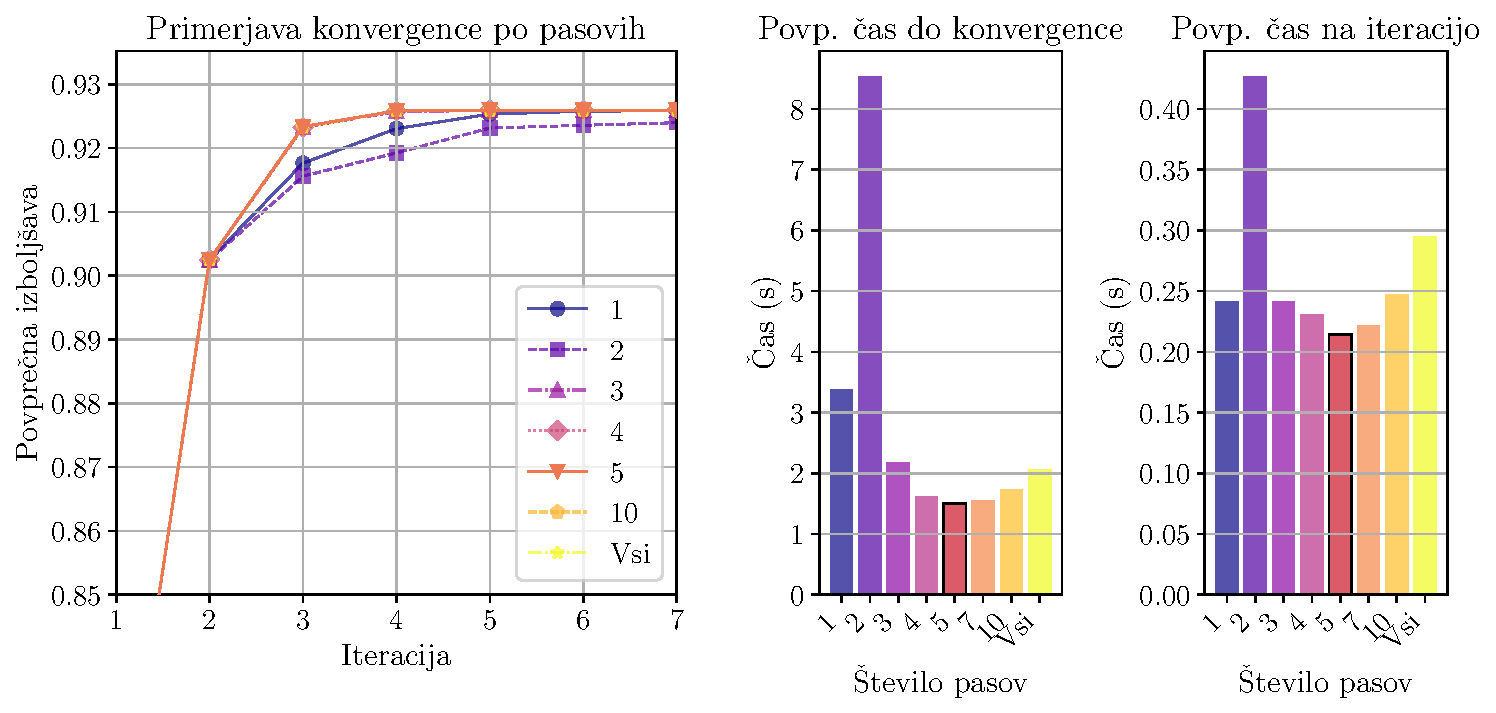
\includegraphics[width=0.99\textwidth]{images/bands_performance_n20.pdf}
    \caption{Vpliv števila izračunanih pasov Hessove matrike na konvergenco za 20 vmesnih točk. Vidimo lahko, da je 5 pasov v tem primeru optimalno za najhitrejši izračun.}
    \label{fig:bands_20}
\end{figure}

\begin{figure}
    \centering
    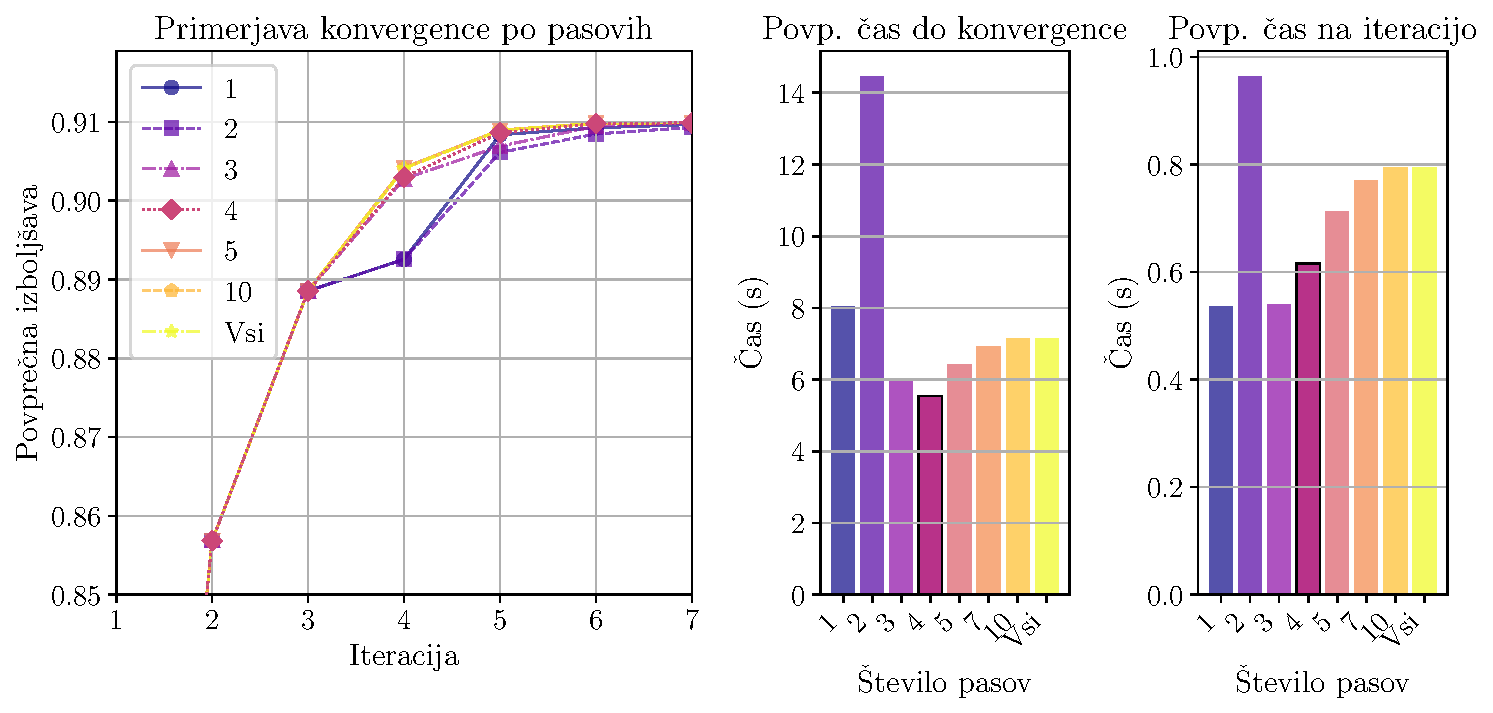
\includegraphics[width=0.99\textwidth]{images/bands_performance_n30.pdf}
    \caption{Vpliv števila izračunanih pasov Hessove matrike na konvergenco za 30 vmesnih točk. Vidimo lahko, da so 4 pasovi v tem primeru optimalno za najhitrejši izračun.}
    \label{fig:bands_30}
\end{figure}

\begin{figure}
    \centering
    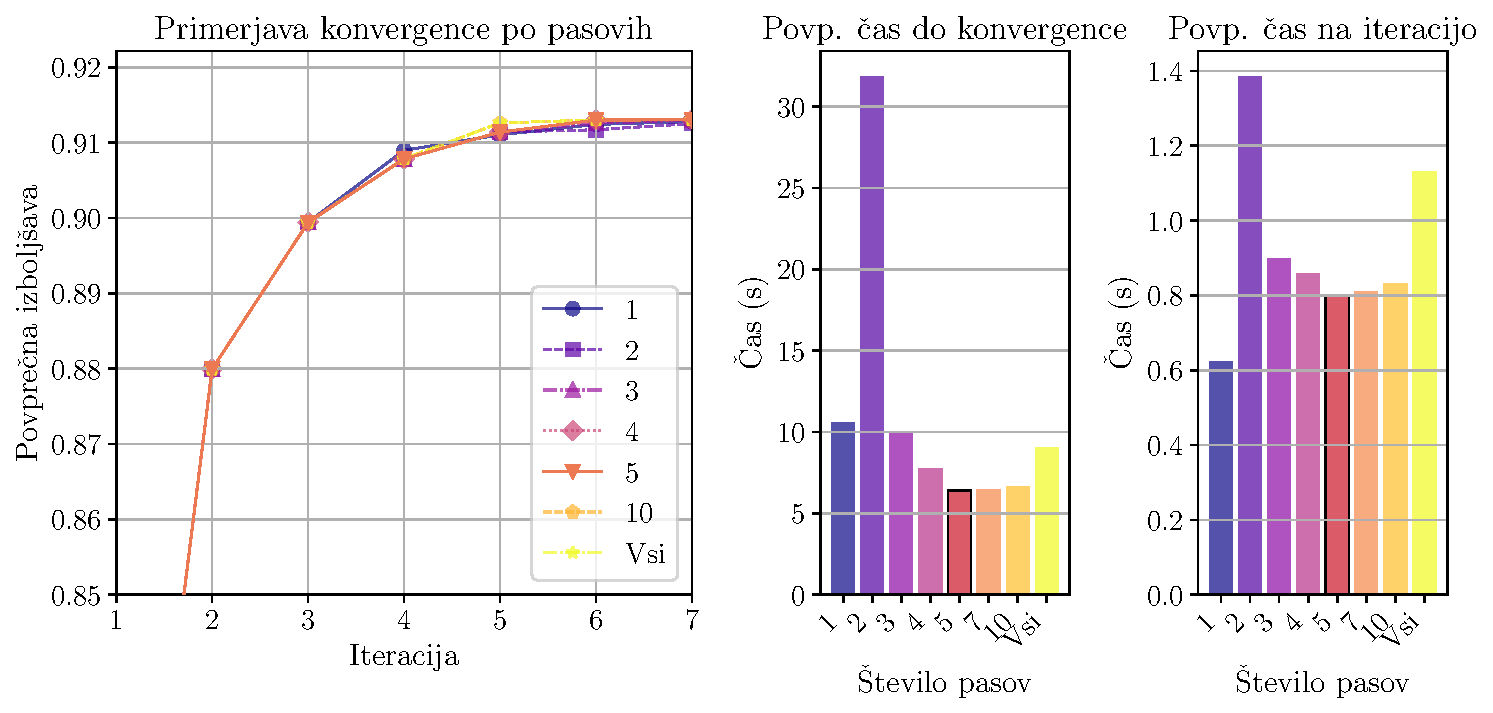
\includegraphics[width=0.99\textwidth]{images/bands_performance_n40.pdf}
    \caption{Vpliv števila izračunanih pasov Hessove matrike na konvergenco za 40 vmesnih točk. Vidimo lahko, da je 5 pasov v tem primeru optimalno za najhitrejši izračun.}
    \label{fig:bands_40}
\end{figure}

\subsection{Hitrost metode v realnem času}

Poleg števila iteracij je za uporabnost metode pomembna tudi učinkovitost v realnem času. Čeprav je Newtonova metoda hitrejša od gradientnega spusta v smislu števila iteracij, je vsaka iteracija računsko zahtevnejša zaradi izračuna Hessove matrike. Sliki~\ref{fig:convergence_time_random} in~\ref{fig:convergence_time_random_and_line} prikazujeta konvergenco v odvisnosti od porabljenega časa (angl. \textit{wall clock time}) za naključno generirane primere, ki smo jih opisali v podpoglavju~\ref{sec:convergence}. Tukaj smo za Newtonovo metodo in Analitični TC pognali algoritem, kjer smo izračunali 5 pasov ob diagonali, da smo zmenjšali računsko zahtevnost. Kljub temu je na grafih razvidno, da v realnem času v obeh primerih Newtonova metoda po večini ni hitrejša od metode z gradientnim spustom. Na grafih, ki prikazujejo primere z 20 vmesnimi točkami ali več, ni prikazana numerična TC metoda, saj je v teh primerih njena konvergenca v realnem času tako počasna, da je pristala izven okvira grafov. Namreč, numerična TC metoda mora na vsakem koraku izvesti evalvacujo cenovne funkcije $(n+1)$-krat, kjer je $n$ število segmentov trajektorije. V našem primeru to pomeni, da mora numerična TC metoda pri vsaki iteraciji rešiti $n+1$ \ac{QP} problemov, da lahko numerično izračuna odvode cenovne funkcije.

Pričakovano se čas izračuna povečuje z večjim številom segmentov trajektorije in v primeru s 40 segmenti presega 2 sekundi, kar je za optimizacijo trajektorij v realnem času preveč. Kljub temu pa ne opazimo bistveno povečane relativne razlike med gradientnim spustom in Newtonovo metodo. Prav tako je dobljeni rezultat na 40 točkah primerljiv z rezultati, ki jih navajajo v \cite{sun2021fast}, kjer je določen delež njihove kode napisan v programskem jeziku C++, kar omogoča hitrejši izračun. Tu priznavamo, da v \cite{sun2021fast} dodatno uporabljajo neenakostne omejitve.

\begin{figure}
    \centering
    % To use in your document:
% \begin{figure}
%     \centering
%     % To use in your document:
% \begin{figure}
%     \centering
%     % To use in your document:
% \begin{figure}
%     \centering
%     \input{tikz/convergence_time_analysis_random.tex}
%     \caption{Časovna analiza konvergence z naključnimi začetnimi točkami}
%     \label{fig:convergence_time_random}
% \end{figure}
\def\yrange{0.15}
\def\ymina{0.37}
\def\yminb{0.57}
\def\yminc{0.58}
\def\ymind{0.6}
\def\ymine{0.6}
\def\width{0.49\textwidth}
\def\plotwidth{0.7\textwidth}
\def\gridstyle{dashed}

\begin{subfigure}[b]{\width}
    \centering
    \begin{tikzpicture}
    \begin{axis}[
        xlabel={Čas [s]},
        ylabel={Povprečna izboljšava},
        xmin=0, xmax=0.3,
        ymin=\ymina, ymax={\ymina+\yrange},
        xmajorgrids=true,
        ymajorgrids=true,
        minor tick num=1,
        grid=both,
        grid style=\gridstyle,
        width=\plotwidth,
        height=5cm,
        scale only axis,
    ]
    \addplot[color=blue, thick] table [x=time, y expr=\thisrow{newton_mean}, col sep=comma] {data/convergence_time_results_random_5.csv};
    \addplot[color=red, thick] table [x=time, y expr=\thisrow{gradient_mean}, col sep=comma] {data/convergence_time_results_random_5.csv};
    \addplot[color=orange, thick] table [x=time, y expr=\thisrow{scipy_mean}, col sep=comma] {data/convergence_time_results_random_5.csv};
    \addplot[color=black!60!green, thick] table [x=time, y expr=\thisrow{trust-constr_mean}, col sep=comma] {data/convergence_time_results_random_5.csv};
    \end{axis}
    \end{tikzpicture}
    \caption{5 točk}
\end{subfigure}
\hfill
\begin{subfigure}[b]{\width}
    \centering
    \begin{tikzpicture}
    \begin{axis}[
        xlabel={Čas [s]},
        ylabel={Povprečna izboljšava},
        xmin=0, xmax=0.5,
        ymin=\yminb, ymax={\yminb+\yrange},
        xmajorgrids=true,
        ymajorgrids=true,
        minor tick num=1,
        grid=both,
        grid style=\gridstyle,
        width=\plotwidth,
        height=5cm,
        scale only axis,
    ]
    \addplot[color=blue, thick] table [x=time, y expr=\thisrow{newton_mean}, col sep=comma] {data/convergence_time_results_random_10.csv};
    \addplot[color=red, thick] table [x=time, y expr=\thisrow{gradient_mean}, col sep=comma] {data/convergence_time_results_random_10.csv};
    \addplot[color=orange, thick] table [x=time, y expr=\thisrow{scipy_mean}, col sep=comma] {data/convergence_time_results_random_10.csv};
    \addplot[color=black!60!green, thick] table [x=time, y expr=\thisrow{trust-constr_mean}, col sep=comma] {data/convergence_time_results_random_10.csv};
    \end{axis}
    \end{tikzpicture}
    \caption{10 točk}
\end{subfigure}

\vspace{0.5cm}

\begin{subfigure}[b]{\width}
    \centering
    \begin{tikzpicture}
    \begin{axis}[
        xlabel={Čas [s]},
        ylabel={Povprečna izboljšava},
        xmin=0, xmax=1.0,
        ymin=\yminc, ymax={\yminc+\yrange},
        xmajorgrids=true,
        ymajorgrids=true,
        minor tick num=1,
        grid=both,
        grid style=\gridstyle,
        width=\plotwidth,
        height=5cm,
        scale only axis,
    ]
    \addplot[color=blue, thick] table [x=time, y expr=\thisrow{newton_mean}, col sep=comma] {data/convergence_time_results_random_20.csv};
    \addplot[color=red, thick] table [x=time, y expr=\thisrow{gradient_mean}, col sep=comma] {data/convergence_time_results_random_20.csv};
    \addplot[color=orange, thick] table [x=time, y expr=\thisrow{scipy_mean}, col sep=comma] {data/convergence_time_results_random_20.csv};
    \addplot[color=black!60!green, thick] table [x=time, y expr=\thisrow{trust-constr_mean}, col sep=comma] {data/convergence_time_results_random_20.csv};
    \end{axis}
    \end{tikzpicture}
    \caption{20 točk}
\end{subfigure}
\hfill
\begin{subfigure}[b]{\width}
    \centering
    \begin{tikzpicture}
    \begin{axis}[
        xlabel={Čas [s]},
        ylabel={Povprečna izboljšava},
        xmin=0, xmax=2.0,
        ymin=\ymind, ymax={\ymind+\yrange},
        xmajorgrids=true,
        ymajorgrids=true,
        minor tick num=1,
        grid=both,
        grid style=\gridstyle,
        width=\plotwidth,
        height=5cm,
        scale only axis,
    ]
    \addplot[color=blue, thick] table [x=time, y expr=\thisrow{newton_mean}, col sep=comma] {data/convergence_time_results_random_30.csv};
    \addplot[color=red, thick] table [x=time, y expr=\thisrow{gradient_mean}, col sep=comma] {data/convergence_time_results_random_30.csv};
    \addplot[color=orange, thick] table [x=time, y expr=\thisrow{scipy_mean}, col sep=comma] {data/convergence_time_results_random_30.csv};
    \addplot[color=black!60!green, thick] table [x=time, y expr=\thisrow{trust-constr_mean}, col sep=comma] {data/convergence_time_results_random_30.csv};
    \end{axis}
    \end{tikzpicture}
    \caption{30 točk}
\end{subfigure}

\vspace{0.5cm}

\begin{subfigure}[b]{\textwidth}
    \centering
    \begin{tikzpicture}
    \begin{axis}[
        xlabel={Čas [s]},
        ylabel={Povprečna izboljšava},
        xmin=0, xmax=4.0,
        ymin=\ymine, ymax={\ymine+\yrange},
        xmajorgrids=true,
        ymajorgrids=true,
        minor tick num=1,
        grid=both,
        grid style=\gridstyle,
        legend style={at={(1.15,0.5)}, anchor=west, draw=none, fill=none},
        width=0.343\textwidth,
        height=5cm,
        scale only axis,
    ]
    \addplot[color=blue, thick] table [x=time, y expr=\thisrow{newton_mean}, col sep=comma] {data/convergence_time_results_random_40.csv};
    \addplot[color=red, thick] table [x=time, y expr=\thisrow{gradient_mean}, col sep=comma] {data/convergence_time_results_random_40.csv};
    \addplot[color=orange, thick] table [x=time, y expr=\thisrow{scipy_mean}, col sep=comma] {data/convergence_time_results_random_40.csv};
    \addplot[color=black!60!green, thick] table [x=time, y expr=\thisrow{trust-constr_mean}, col sep=comma] {data/convergence_time_results_random_40.csv};
    \legend{Newton, Gradient, Numerični TC, Analitični TC}
    \end{axis}
    \end{tikzpicture}
    \caption{40 točk}
\end{subfigure}

%     \caption{Časovna analiza konvergence z naključnimi začetnimi točkami}
%     \label{fig:convergence_time_random}
% \end{figure}
\def\yrange{0.15}
\def\ymina{0.37}
\def\yminb{0.57}
\def\yminc{0.58}
\def\ymind{0.6}
\def\ymine{0.6}
\def\width{0.49\textwidth}
\def\plotwidth{0.7\textwidth}
\def\gridstyle{dashed}

\begin{subfigure}[b]{\width}
    \centering
    \begin{tikzpicture}
    \begin{axis}[
        xlabel={Čas [s]},
        ylabel={Povprečna izboljšava},
        xmin=0, xmax=0.3,
        ymin=\ymina, ymax={\ymina+\yrange},
        xmajorgrids=true,
        ymajorgrids=true,
        minor tick num=1,
        grid=both,
        grid style=\gridstyle,
        width=\plotwidth,
        height=5cm,
        scale only axis,
    ]
    \addplot[color=blue, thick] table [x=time, y expr=\thisrow{newton_mean}, col sep=comma] {data/convergence_time_results_random_5.csv};
    \addplot[color=red, thick] table [x=time, y expr=\thisrow{gradient_mean}, col sep=comma] {data/convergence_time_results_random_5.csv};
    \addplot[color=orange, thick] table [x=time, y expr=\thisrow{scipy_mean}, col sep=comma] {data/convergence_time_results_random_5.csv};
    \addplot[color=black!60!green, thick] table [x=time, y expr=\thisrow{trust-constr_mean}, col sep=comma] {data/convergence_time_results_random_5.csv};
    \end{axis}
    \end{tikzpicture}
    \caption{5 točk}
\end{subfigure}
\hfill
\begin{subfigure}[b]{\width}
    \centering
    \begin{tikzpicture}
    \begin{axis}[
        xlabel={Čas [s]},
        ylabel={Povprečna izboljšava},
        xmin=0, xmax=0.5,
        ymin=\yminb, ymax={\yminb+\yrange},
        xmajorgrids=true,
        ymajorgrids=true,
        minor tick num=1,
        grid=both,
        grid style=\gridstyle,
        width=\plotwidth,
        height=5cm,
        scale only axis,
    ]
    \addplot[color=blue, thick] table [x=time, y expr=\thisrow{newton_mean}, col sep=comma] {data/convergence_time_results_random_10.csv};
    \addplot[color=red, thick] table [x=time, y expr=\thisrow{gradient_mean}, col sep=comma] {data/convergence_time_results_random_10.csv};
    \addplot[color=orange, thick] table [x=time, y expr=\thisrow{scipy_mean}, col sep=comma] {data/convergence_time_results_random_10.csv};
    \addplot[color=black!60!green, thick] table [x=time, y expr=\thisrow{trust-constr_mean}, col sep=comma] {data/convergence_time_results_random_10.csv};
    \end{axis}
    \end{tikzpicture}
    \caption{10 točk}
\end{subfigure}

\vspace{0.5cm}

\begin{subfigure}[b]{\width}
    \centering
    \begin{tikzpicture}
    \begin{axis}[
        xlabel={Čas [s]},
        ylabel={Povprečna izboljšava},
        xmin=0, xmax=1.0,
        ymin=\yminc, ymax={\yminc+\yrange},
        xmajorgrids=true,
        ymajorgrids=true,
        minor tick num=1,
        grid=both,
        grid style=\gridstyle,
        width=\plotwidth,
        height=5cm,
        scale only axis,
    ]
    \addplot[color=blue, thick] table [x=time, y expr=\thisrow{newton_mean}, col sep=comma] {data/convergence_time_results_random_20.csv};
    \addplot[color=red, thick] table [x=time, y expr=\thisrow{gradient_mean}, col sep=comma] {data/convergence_time_results_random_20.csv};
    \addplot[color=orange, thick] table [x=time, y expr=\thisrow{scipy_mean}, col sep=comma] {data/convergence_time_results_random_20.csv};
    \addplot[color=black!60!green, thick] table [x=time, y expr=\thisrow{trust-constr_mean}, col sep=comma] {data/convergence_time_results_random_20.csv};
    \end{axis}
    \end{tikzpicture}
    \caption{20 točk}
\end{subfigure}
\hfill
\begin{subfigure}[b]{\width}
    \centering
    \begin{tikzpicture}
    \begin{axis}[
        xlabel={Čas [s]},
        ylabel={Povprečna izboljšava},
        xmin=0, xmax=2.0,
        ymin=\ymind, ymax={\ymind+\yrange},
        xmajorgrids=true,
        ymajorgrids=true,
        minor tick num=1,
        grid=both,
        grid style=\gridstyle,
        width=\plotwidth,
        height=5cm,
        scale only axis,
    ]
    \addplot[color=blue, thick] table [x=time, y expr=\thisrow{newton_mean}, col sep=comma] {data/convergence_time_results_random_30.csv};
    \addplot[color=red, thick] table [x=time, y expr=\thisrow{gradient_mean}, col sep=comma] {data/convergence_time_results_random_30.csv};
    \addplot[color=orange, thick] table [x=time, y expr=\thisrow{scipy_mean}, col sep=comma] {data/convergence_time_results_random_30.csv};
    \addplot[color=black!60!green, thick] table [x=time, y expr=\thisrow{trust-constr_mean}, col sep=comma] {data/convergence_time_results_random_30.csv};
    \end{axis}
    \end{tikzpicture}
    \caption{30 točk}
\end{subfigure}

\vspace{0.5cm}

\begin{subfigure}[b]{\textwidth}
    \centering
    \begin{tikzpicture}
    \begin{axis}[
        xlabel={Čas [s]},
        ylabel={Povprečna izboljšava},
        xmin=0, xmax=4.0,
        ymin=\ymine, ymax={\ymine+\yrange},
        xmajorgrids=true,
        ymajorgrids=true,
        minor tick num=1,
        grid=both,
        grid style=\gridstyle,
        legend style={at={(1.15,0.5)}, anchor=west, draw=none, fill=none},
        width=0.343\textwidth,
        height=5cm,
        scale only axis,
    ]
    \addplot[color=blue, thick] table [x=time, y expr=\thisrow{newton_mean}, col sep=comma] {data/convergence_time_results_random_40.csv};
    \addplot[color=red, thick] table [x=time, y expr=\thisrow{gradient_mean}, col sep=comma] {data/convergence_time_results_random_40.csv};
    \addplot[color=orange, thick] table [x=time, y expr=\thisrow{scipy_mean}, col sep=comma] {data/convergence_time_results_random_40.csv};
    \addplot[color=black!60!green, thick] table [x=time, y expr=\thisrow{trust-constr_mean}, col sep=comma] {data/convergence_time_results_random_40.csv};
    \legend{Newton, Gradient, Numerični TC, Analitični TC}
    \end{axis}
    \end{tikzpicture}
    \caption{40 točk}
\end{subfigure}

%     \caption{Časovna analiza konvergence z naključnimi začetnimi točkami}
%     \label{fig:convergence_time_random}
% \end{figure}
\def\yrange{0.15}
\def\ymina{0.37}
\def\yminb{0.57}
\def\yminc{0.58}
\def\ymind{0.6}
\def\ymine{0.6}
\def\width{0.49\textwidth}
\def\plotwidth{0.7\textwidth}
\def\gridstyle{dashed}

\begin{subfigure}[b]{\width}
    \centering
    \begin{tikzpicture}
    \begin{axis}[
        xlabel={Čas [s]},
        ylabel={Povprečna izboljšava},
        xmin=0, xmax=0.3,
        ymin=\ymina, ymax={\ymina+\yrange},
        xmajorgrids=true,
        ymajorgrids=true,
        minor tick num=1,
        grid=both,
        grid style=\gridstyle,
        width=\plotwidth,
        height=5cm,
        scale only axis,
    ]
    \addplot[color=blue, thick] table [x=time, y expr=\thisrow{newton_mean}, col sep=comma] {data/convergence_time_results_random_5.csv};
    \addplot[color=red, thick] table [x=time, y expr=\thisrow{gradient_mean}, col sep=comma] {data/convergence_time_results_random_5.csv};
    \addplot[color=orange, thick] table [x=time, y expr=\thisrow{scipy_mean}, col sep=comma] {data/convergence_time_results_random_5.csv};
    \addplot[color=black!60!green, thick] table [x=time, y expr=\thisrow{trust-constr_mean}, col sep=comma] {data/convergence_time_results_random_5.csv};
    \end{axis}
    \end{tikzpicture}
    \caption{5 točk}
\end{subfigure}
\hfill
\begin{subfigure}[b]{\width}
    \centering
    \begin{tikzpicture}
    \begin{axis}[
        xlabel={Čas [s]},
        ylabel={Povprečna izboljšava},
        xmin=0, xmax=0.5,
        ymin=\yminb, ymax={\yminb+\yrange},
        xmajorgrids=true,
        ymajorgrids=true,
        minor tick num=1,
        grid=both,
        grid style=\gridstyle,
        width=\plotwidth,
        height=5cm,
        scale only axis,
    ]
    \addplot[color=blue, thick] table [x=time, y expr=\thisrow{newton_mean}, col sep=comma] {data/convergence_time_results_random_10.csv};
    \addplot[color=red, thick] table [x=time, y expr=\thisrow{gradient_mean}, col sep=comma] {data/convergence_time_results_random_10.csv};
    \addplot[color=orange, thick] table [x=time, y expr=\thisrow{scipy_mean}, col sep=comma] {data/convergence_time_results_random_10.csv};
    \addplot[color=black!60!green, thick] table [x=time, y expr=\thisrow{trust-constr_mean}, col sep=comma] {data/convergence_time_results_random_10.csv};
    \end{axis}
    \end{tikzpicture}
    \caption{10 točk}
\end{subfigure}

\vspace{0.5cm}

\begin{subfigure}[b]{\width}
    \centering
    \begin{tikzpicture}
    \begin{axis}[
        xlabel={Čas [s]},
        ylabel={Povprečna izboljšava},
        xmin=0, xmax=1.0,
        ymin=\yminc, ymax={\yminc+\yrange},
        xmajorgrids=true,
        ymajorgrids=true,
        minor tick num=1,
        grid=both,
        grid style=\gridstyle,
        width=\plotwidth,
        height=5cm,
        scale only axis,
    ]
    \addplot[color=blue, thick] table [x=time, y expr=\thisrow{newton_mean}, col sep=comma] {data/convergence_time_results_random_20.csv};
    \addplot[color=red, thick] table [x=time, y expr=\thisrow{gradient_mean}, col sep=comma] {data/convergence_time_results_random_20.csv};
    \addplot[color=orange, thick] table [x=time, y expr=\thisrow{scipy_mean}, col sep=comma] {data/convergence_time_results_random_20.csv};
    \addplot[color=black!60!green, thick] table [x=time, y expr=\thisrow{trust-constr_mean}, col sep=comma] {data/convergence_time_results_random_20.csv};
    \end{axis}
    \end{tikzpicture}
    \caption{20 točk}
\end{subfigure}
\hfill
\begin{subfigure}[b]{\width}
    \centering
    \begin{tikzpicture}
    \begin{axis}[
        xlabel={Čas [s]},
        ylabel={Povprečna izboljšava},
        xmin=0, xmax=2.0,
        ymin=\ymind, ymax={\ymind+\yrange},
        xmajorgrids=true,
        ymajorgrids=true,
        minor tick num=1,
        grid=both,
        grid style=\gridstyle,
        width=\plotwidth,
        height=5cm,
        scale only axis,
    ]
    \addplot[color=blue, thick] table [x=time, y expr=\thisrow{newton_mean}, col sep=comma] {data/convergence_time_results_random_30.csv};
    \addplot[color=red, thick] table [x=time, y expr=\thisrow{gradient_mean}, col sep=comma] {data/convergence_time_results_random_30.csv};
    \addplot[color=orange, thick] table [x=time, y expr=\thisrow{scipy_mean}, col sep=comma] {data/convergence_time_results_random_30.csv};
    \addplot[color=black!60!green, thick] table [x=time, y expr=\thisrow{trust-constr_mean}, col sep=comma] {data/convergence_time_results_random_30.csv};
    \end{axis}
    \end{tikzpicture}
    \caption{30 točk}
\end{subfigure}

\vspace{0.5cm}

\begin{subfigure}[b]{\textwidth}
    \centering
    \begin{tikzpicture}
    \begin{axis}[
        xlabel={Čas [s]},
        ylabel={Povprečna izboljšava},
        xmin=0, xmax=4.0,
        ymin=\ymine, ymax={\ymine+\yrange},
        xmajorgrids=true,
        ymajorgrids=true,
        minor tick num=1,
        grid=both,
        grid style=\gridstyle,
        legend style={at={(1.15,0.5)}, anchor=west, draw=none, fill=none},
        width=0.343\textwidth,
        height=5cm,
        scale only axis,
    ]
    \addplot[color=blue, thick] table [x=time, y expr=\thisrow{newton_mean}, col sep=comma] {data/convergence_time_results_random_40.csv};
    \addplot[color=red, thick] table [x=time, y expr=\thisrow{gradient_mean}, col sep=comma] {data/convergence_time_results_random_40.csv};
    \addplot[color=orange, thick] table [x=time, y expr=\thisrow{scipy_mean}, col sep=comma] {data/convergence_time_results_random_40.csv};
    \addplot[color=black!60!green, thick] table [x=time, y expr=\thisrow{trust-constr_mean}, col sep=comma] {data/convergence_time_results_random_40.csv};
    \legend{Newton, Gradient, Numerični TC, Analitični TC}
    \end{axis}
    \end{tikzpicture}
    \caption{40 točk}
\end{subfigure}

    \caption{Časovna konvergenca z naključnimi začetnimi točkami}
    \label{fig:convergence_time_random}
\end{figure}

\begin{figure}
    \centering
    \input{tikz/convergence_time_analysis_random_and_line.tex}
    \caption{Časovna konvergenca z naključnimi točkami in premicami}
    \label{fig:convergence_time_random_and_line}
\end{figure}







\section{Zaključek}
\label{sec:zakljucek}

V tem magistrskem delu smo predstavili Newtonovo metodo za optimizacijo trajektorij za diferencialno ploščate sisteme. Pokazali smo, kako minimizacijo funkcionala z omejitvami pretvorimo v dvonivojski optimizacijski problem, kjer ima nižjenivojski problem strukturo \ac{QP} z enakostnimi omejitvami. S pomočjo \ac{IIF} smo pokazali, da lahko analitično izračunamo gradient in Hessovo matriko cenovne funkcije zgornjenivojskega problema. Z eksperimenti smo pokazali, da Newtonova metoda potrebuje manj iteracij za konvergenco kot metoda, ki uporablja samo gradient ali metoda, ki odvode izračuna numerično. Kljub temu v večini primerov Newtonova metoda v realnem času ni hitrejša od gradientnega spusta. Opisali smo tudi nekaj pristopov za pohitritev algoritma, ki izrabljajo strukturo problema.

Ostaja mnogo poti za izboljšavo. Glavni izmed njih je vključitev neenakostnih omejitev v \ac{QP}, kar bi omogočilo načrtovanje trajektorij z izogibanjem preprekam in omejitev maksimalnih hitrosti in pospeškov kvadrotorjev. To bi sicer lahko pripeljalo do težav pri veljavnosti \ac{IIF}, vendar v \cite{sun2021fast, amos2017optnet} že ponudijo rešitve. Dodatno bi bilo zanimivo raziskati vključitev nelinearnih omejitev, npr. omejitev stožca drugega reda, ki bi bile koristne za omejitve hitrosti in pospeška; za to bi bilo treba uporabiti algoritme za semidiefinitno programiranje, kot je npr. Clarabel \cite{goulart2024clarabel} oz. CuClarabel \cite{chen2024cuclarabel}, ki deluje z grafičnimi procesnimi enotami. Nadalje, implementacija v nižjenivojskem jeziku, kot je C++, bi z veliko verjetnostjo bistveno izboljšala hitrost. Normalizacija časovnih intervalov, kot so jo predlagali v \cite{mellinger2011minimum}, bi pripomogla k večji stabilnosti metode. Uporaba metode ničelnega prostora za faktorizacijo matrike v enačbi~\eqref{eq:kkt_matrix} \cite{rees2014null} bi lahko pripomogla k dodatni pohitritvi. Na strani implementacije bi bilo koristno dodati tudi nastavljive parametre za npr. začetne/končne odvode trajektorije. Še en zanimiv pristop k boljši hitrosti bi bil razvoj metode globokega učenja za aproksimacijo gradienta in Hessove matrike oz. optimizacijskega koraka; v preteklosti se je tak pristop izkazal za zelo učinkovit pri pospeševanju optimizacijskih algoritmov \cite{andrychowicz2016learning}. Na koncu bi bilo zanimivo raziskati, ali se podobna metoda lahko uporabi tudi v problemih na drugih področjih.


%\subsection{Sklicevanje in citiranje}
%Za sklice uporabljamo \verb|\ref|, za sklice na enačbe \verb|\eqref|, za citate \verb|\cite|. Pri
%sklicevanju in citiranju sklicano številko povežemo s prejšnjo besedo z nedeljivim presledkom
%$\sim$, kot npr.\ \verb|iz trditve~\ref{trd:obstoj-omega} vidimo|.

%\begin{primer}
%  Zaporedje~\eqref{eq:zero-kompleks} iz dokaza trditve~\ref{trd:obstoj-omega} na
%  strani~\pageref{trd:obstoj-omega} lahko najdemo tudi v Spletni enciklopediji zaporedij~\cite{oeis}.
%  Citiramo lahko tudi bolj natančno~\cite[trditev 2.1, str.\ 23]{lebedev2009introduction}.
%\end{primer}







%\subsection{Kako narediti stvarno kazalo}
%Dodate ukaze \verb|\index{polje}| na besede, kjer je pojavijo, kot tukaj\index{tukaj}.
%Več o stvarnih kazalih je na voljo na \url{https://en.wikibooks.org/wiki/LaTeX/Indexing}.

%\subsection{Navajanje literature}
%Članke citiramo z uporabo \verb|\cite{label}|, \verb|\cite[text]{label}| ali pa več naenkrat s
%\verb|\cite\{label1, label2}|. Tudi tukaj predhodno besedo in citat povežemo z nedeljivim presledkom
%$\sim$. Na primer~\cite{chen2006meshless,liu2001point}, ali pa \cite{kibriya2007empirical}, ali pa
%\cite[str.\ 12]{trobec2015parallel}, \cite[enačba (2.3)]{pereira2016convergence}.
%Vnosi iz \verb|.bib| datoteke, ki niso citirani, se ne prikažejo v seznamu literature, zato jih
%tukaj citiram.~\cite{vene2000categorical}, \cite{gregoric2017stopniceni}, \cite{slak2015induktivni},
%\cite{nsphere}, \cite{kearsley1975linearly}, \cite{STtemplate}, \cite{NunbergerTand}, \cite{vanoosten2008realizability}.

\appendix

\section{Primer}
\label{app:example}
V tem dodatku predstavimo ilustrativen primer, ki služi boljšemu razumevanju opisane metode na konkretnem problemu. Najprej opišemo konstrukcijo QP s fiksnimi časi segmentov, nato pa še izračun komponent gradient cenovne funkcije $F(\tvec)$. Na koncu si ogledamo še projekcijo gradienta na podprostor $\lbrace \tvec : \mathbf{1}^\top \tvec = 0 \rbrace$. Izračun Hessove matrike izpustimo.

\subsection{QP}

Za boljše razumevanje konstrukcije QP s fiksnimi časi segmentov si oglejmo primer z $n = 2$ segmentoma, stopnjo polinomskih zlepkov $d = 4$, redom zveznosti $K = 2$ in optimizacijsko stopnjo odvoda $r = 3$. Optimizirali bomo trajektorijo v dveh dimenzijah, $x$ in $y$, pri čemer bomo uporabili sledeče vmesne točke in čase segmentov:
\begin{equation}
\begin{aligned}
P_0 &= (1, 0) \\
P_1 &= (1, 1) \\
P_2 &= (2, 0) \\
\tvec &= (1, 2)
\end{aligned}
\end{equation}
Torej, med točko $P_0$ in $P_1$ bomo potovali $1s$, med točko $P_1$ in $P_2$ pa $2s$. Sedaj bomo izračunali matriko $\mathbf{Q}$, ki bo imela bločno diagonalno strukturo:
\begin{equation}
\mathbf{Q} = 
\begin{bNiceMatrix}[columns-width=1.2em]
\textcolor{block1color}{0} & \textcolor{block1color}{0} & \textcolor{block1color}{0} & \textcolor{block1color}{0} & \textcolor{block1color}{0} & 0 & 0 & 0 & 0 & 0 \\
\textcolor{block1color}{0} & \textcolor{block1color}{0} & \textcolor{block1color}{0} & \textcolor{block1color}{0} & \textcolor{block1color}{0} & 0 & 0 & 0 & 0 & 0 \\
\textcolor{block1color}{0} & \textcolor{block1color}{0} & \textcolor{block1color}{0} & \textcolor{block1color}{0} & \textcolor{block1color}{0} & 0 & 0 & 0 & 0 & 0 \\
\textcolor{block1color}{0} & \textcolor{block1color}{0} & \textcolor{block1color}{0} & \textcolor{block1color}{36} & \textcolor{block1color}{72} & 0 & 0 & 0 & 0 & 0 \\
\textcolor{block1color}{0} & \textcolor{block1color}{0} & \textcolor{block1color}{0} & \textcolor{block1color}{72} & \textcolor{block1color}{192} & 0 & 0 & 0 & 0 & 0 \\
0 & 0 & 0 & 0 & 0 & \textcolor{block2color}{0} & \textcolor{block2color}{0} & \textcolor{block2color}{0} & \textcolor{block2color}{0} & \textcolor{block2color}{0} \\
0 & 0 & 0 & 0 & 0 & \textcolor{block2color}{0} & \textcolor{block2color}{0} & \textcolor{block2color}{0} & \textcolor{block2color}{0} & \textcolor{block2color}{0} \\
0 & 0 & 0 & 0 & 0 & \textcolor{block2color}{0} & \textcolor{block2color}{0} & \textcolor{block2color}{0} & \textcolor{block2color}{0} & \textcolor{block2color}{0} \\
0 & 0 & 0 & 0 & 0 & \textcolor{block2color}{0} & \textcolor{block2color}{0} & \textcolor{block2color}{0} & \textcolor{block2color}{72} & \textcolor{block2color}{288} \\
0 & 0 & 0 & 0 & 0 & \textcolor{block2color}{0} & \textcolor{block2color}{0} & \textcolor{block2color}{0} & \textcolor{block2color}{288} & \textcolor{block2color}{1536}
\end{bNiceMatrix}
\end{equation}

Če eksplicitno zapišemo odvisnost od časov $t_1$ in $t_2$, dobimo:
\begin{equation}
\mathbf{Q}(\tvec) = 
\begin{bNiceMatrix}[columns-width=auto]
\textcolor{block1color}{0} & \textcolor{block1color}{0} & \textcolor{block1color}{0} & \textcolor{block1color}{0} & \textcolor{block1color}{0} & 0 & 0 & 0 & 0 & 0 \\
\textcolor{block1color}{0} & \textcolor{block1color}{0} & \textcolor{block1color}{0} & \textcolor{block1color}{0} & \textcolor{block1color}{0} & 0 & 0 & 0 & 0 & 0 \\
\textcolor{block1color}{0} & \textcolor{block1color}{0} & \textcolor{block1color}{0} & \textcolor{block1color}{0} & \textcolor{block1color}{0} & 0 & 0 & 0 & 0 & 0 \\
\textcolor{block1color}{0} & \textcolor{block1color}{0} & \textcolor{block1color}{0} & \textcolor{block1color}{36 t_1} & \textcolor{block1color}{72 t_1^2} & 0 & 0 & 0 & 0 & 0 \\
\textcolor{block1color}{0} & \textcolor{block1color}{0} & \textcolor{block1color}{0} & \textcolor{block1color}{72 t_1^2} & \textcolor{block1color}{192 t_1^3} & 0 & 0 & 0 & 0 & 0 \\
0 & 0 & 0 & 0 & 0 & \textcolor{block2color}{0} & \textcolor{block2color}{0} & \textcolor{block2color}{0} & \textcolor{block2color}{0} & \textcolor{block2color}{0} \\
0 & 0 & 0 & 0 & 0 & \textcolor{block2color}{0} & \textcolor{block2color}{0} & \textcolor{block2color}{0} & \textcolor{block2color}{0} & \textcolor{block2color}{0} \\
0 & 0 & 0 & 0 & 0 & \textcolor{block2color}{0} & \textcolor{block2color}{0} & \textcolor{block2color}{0} & \textcolor{block2color}{0} & \textcolor{block2color}{0} \\
0 & 0 & 0 & 0 & 0 & \textcolor{block2color}{0} & \textcolor{block2color}{0} & \textcolor{block2color}{0} & \textcolor{block2color}{36 t_2} & \textcolor{block2color}{72 t_2^2} \\
0 & 0 & 0 & 0 & 0 & \textcolor{block2color}{0} & \textcolor{block2color}{0} & \textcolor{block2color}{0} & \textcolor{block2color}{72 t_2^2} & \textcolor{block2color}{192 t_2^3}
\end{bNiceMatrix}
\end{equation}

Matriko $\amat$ izračunamo na podlagi strukture, opisane v prejšnjem podpoglavju. Za naš primer z dvema segmentoma in omejitvami do drugega odvoda dobimo:
\begin{equation}
\amat = 
\begin{bNiceMatrix}[columns-width=1.2em]
\textcolor{block3color}{1} & \textcolor{block3color}{0} & \textcolor{block3color}{0} & \textcolor{block3color}{0} & \textcolor{block3color}{0} & 0 & 0 & 0 & 0 & 0 \\
\textcolor{block3color}{0} & \textcolor{block3color}{1} & \textcolor{block3color}{0} & \textcolor{block3color}{0} & \textcolor{block3color}{0} & 0 & 0 & 0 & 0 & 0 \\
\textcolor{block3color}{0} & \textcolor{block3color}{0} & \textcolor{block3color}{2} & \textcolor{block3color}{0} & \textcolor{block3color}{0} & 0 & 0 & 0 & 0 & 0 \\
\textcolor{block4color}{1} & \textcolor{block4color}{1} & \textcolor{block4color}{1} & \textcolor{block4color}{1} & \textcolor{block4color}{1} & \textcolor{block5color}{-1} & \textcolor{block5color}{0} & \textcolor{block5color}{0} & \textcolor{block5color}{0} & \textcolor{block5color}{0} \\
\textcolor{block4color}{0} & \textcolor{block4color}{1} & \textcolor{block4color}{2} & \textcolor{block4color}{3} & \textcolor{block4color}{4} & \textcolor{block5color}{0} & \textcolor{block5color}{-1} & \textcolor{block5color}{0} & \textcolor{block5color}{0} & \textcolor{block5color}{0} \\
\textcolor{block4color}{0} & \textcolor{block4color}{0} & \textcolor{block4color}{2} & \textcolor{block4color}{6} & \textcolor{block4color}{12} & \textcolor{block5color}{0} & \textcolor{block5color}{0} & \textcolor{block5color}{-2} & \textcolor{block5color}{0} & \textcolor{block5color}{0} \\
\textcolor{block4color}{0} & \textcolor{block4color}{0} & \textcolor{block4color}{0} & \textcolor{block4color}{0} & \textcolor{block4color}{0} & \textcolor{block5color}{1} & \textcolor{block5color}{0} & \textcolor{block5color}{0} & \textcolor{block5color}{0} & \textcolor{block5color}{0} \\
0 & 0 & 0 & 0 & 0 & \textcolor{block6color}{1} & \textcolor{block6color}{2} & \textcolor{block6color}{4} & \textcolor{block6color}{8} & \textcolor{block6color}{16} \\
0 & 0 & 0 & 0 & 0 & \textcolor{block6color}{0} & \textcolor{block6color}{1} & \textcolor{block6color}{4} & \textcolor{block6color}{12} & \textcolor{block6color}{32} \\
0 & 0 & 0 & 0 & 0 & \textcolor{block6color}{0} & \textcolor{block6color}{0} & \textcolor{block6color}{2} & \textcolor{block6color}{12} & \textcolor{block6color}{48}
\end{bNiceMatrix}
\end{equation}

Če eksplicitno zapišemo odvisnost od časov $t_1$ in $t_2$, dobimo:
{\footnotesize
\begin{equation}
\amat(\tvec) = 
\begin{bNiceMatrix}[columns-width=0.5em]
\textcolor{block3color}{1 \cdot 0^0} & \textcolor{block3color}{1 \cdot 0^1} & \textcolor{block3color}{1 \cdot 0^2} & \textcolor{block3color}{1 \cdot 0^3} & \textcolor{block3color}{1 \cdot 0^4} & 0 & 0 & 0 & 0 & 0 \\
\textcolor{block3color}{0} & \textcolor{block3color}{1 \cdot 0^0} & \textcolor{block3color}{2 \cdot 0^1} & \textcolor{block3color}{3 \cdot 0^2} & \textcolor{block3color}{4 \cdot 0^3} & 0 & 0 & 0 & 0 & 0 \\
\textcolor{block3color}{0} & \textcolor{block3color}{0} & \textcolor{block3color}{2 \cdot 0^0} & \textcolor{block3color}{6 \cdot 0^1} & \textcolor{block3color}{12 \cdot 0^2} & 0 & 0 & 0 & 0 & 0 \\
\textcolor{block4color}{1 \cdot t_1^0} & \textcolor{block4color}{1 \cdot t_1^1} & \textcolor{block4color}{1 \cdot t_1^2} & \textcolor{block4color}{1 \cdot t_1^3} & \textcolor{block4color}{1 \cdot t_1^4} & \textcolor{block5color}{-1 \cdot 0^0} & \textcolor{block5color}{-1 \cdot 0^1} & \textcolor{block5color}{-1 \cdot 0^2} & \textcolor{block5color}{-1 \cdot 0^3} & \textcolor{block5color}{-1 \cdot 0^4} \\
\textcolor{block4color}{0} & \textcolor{block4color}{1 \cdot t_1^0} & \textcolor{block4color}{2 \cdot t_1^1} & \textcolor{block4color}{3 \cdot t_1^2} & \textcolor{block4color}{4 \cdot t_1^3} & \textcolor{block5color}{0} & \textcolor{block5color}{-1 \cdot 0^0} & \textcolor{block5color}{-2 \cdot 0^1} & \textcolor{block5color}{-3 \cdot 0^2} & \textcolor{block5color}{-4 \cdot 0^3} \\
\textcolor{block4color}{0} & \textcolor{block4color}{0} & \textcolor{block4color}{2 \cdot t_1^0} & \textcolor{block4color}{6 \cdot t_1^1} & \textcolor{block4color}{12 \cdot t_1^2} & \textcolor{block5color}{0} & \textcolor{block5color}{0} & \textcolor{block5color}{-2 \cdot 0^0} & \textcolor{block5color}{-6 \cdot 0^1} & \textcolor{block5color}{-12 \cdot 0^2} \\
\textcolor{block4color}{0} & \textcolor{block4color}{0} & \textcolor{block4color}{0} & \textcolor{block4color}{0} & \textcolor{block4color}{0} & \textcolor{block5color}{1 \cdot 0^0} & \textcolor{block5color}{1 \cdot 0^1} & \textcolor{block5color}{1 \cdot 0^2} & \textcolor{block5color}{1 \cdot 0^3} & \textcolor{block5color}{1 \cdot 0^4} \\
0 & 0 & 0 & 0 & 0 & \textcolor{block6color}{1 \cdot t_2^0} & \textcolor{block6color}{1 \cdot t_2^1} & \textcolor{block6color}{1 \cdot t_2^2} & \textcolor{block6color}{1 \cdot t_2^3} & \textcolor{block6color}{1 \cdot t_2^4} \\
0 & 0 & 0 & 0 & 0 & \textcolor{block6color}{0} & \textcolor{block6color}{1 \cdot t_2^0} & \textcolor{block6color}{2 \cdot t_2^1} & \textcolor{block6color}{3 \cdot t_2^2} & \textcolor{block6color}{4 \cdot t_2^3} \\
0 & 0 & 0 & 0 & 0 & \textcolor{block6color}{0} & \textcolor{block6color}{0} & \textcolor{block6color}{2 \cdot t_2^0} & \textcolor{block6color}{6 \cdot t_2^1} & \textcolor{block6color}{12 \cdot t_2^2}
\end{bNiceMatrix}
\end{equation}
}

Vektorja $\bvec$ za $x$ in $y$ dimenziji sta:
\begin{equation}
\bvec_x = \begin{bmatrix} \textcolor{block3color}{1} & \textcolor{block3color}{0} & \textcolor{block3color}{0} & \textcolor{block4color}{0} & \textcolor{block4color}{0} & \textcolor{block4color}{0} & \textcolor{block4color}{1} & \textcolor{block6color}{2} & \textcolor{block6color}{0} & \textcolor{block6color}{0} \end{bmatrix}^\top, \quad
\bvec_y = \begin{bmatrix} \textcolor{block3color}{0} & \textcolor{block3color}{0} & \textcolor{block3color}{0} & \textcolor{block4color}{0} & \textcolor{block4color}{0} & \textcolor{block4color}{0} & \textcolor{block4color}{1} & \textcolor{block6color}{0} & \textcolor{block6color}{0} & \textcolor{block6color}{0} \end{bmatrix}^\top
\end{equation}

Pri tem smo z različnimi barvami poudarili bločno strukturo matrik in določili bloke $\textcolor{block1color}{\mathbf{Q}_1(t_1)}$, $\textcolor{block2color}{\mathbf{Q}_2(t_2)}$, $\textcolor{block3color}{\amat_1(0)}$, $\textcolor{block4color}{\left[{\amat_1(t_1)} \text{ } {-\amat_2(0)}\right]}$ in $\textcolor{block6color}{\amat_2(t_2)}$.

Sedaj lahko ločeno rešimo QP za $x$ in $y$ dimenzijo:
\begin{equation}
    \begin{aligned}
        \min_{\avec_x} & \quad \frac{1}{2}\avec_x^\top \qmat \avec_x & \qquad & \min_{\avec_y} & \quad \frac{1}{2}\avec_y^\top \qmat \avec_y\\
        \text{p.p.} & \quad \amat \avec_x = \bvec_x & & \text{p.p.} & \quad \amat \avec_y = \bvec_y
    \end{aligned}
\end{equation}

Rezultat optimizacije sta vektorja $\avec_x$ in $\avec_y$, ki vsebujeta koeficiente polinomskih zlepkov za $x$ in $y$ dimenzijo. S temi koeficienti lahko nato rekonstruiramo polinomske zlepke in jih združimo v celotno trajektorijo, ki je vidna na sliki~\ref{fig:2segment}.

\begin{figure}
    \centering
    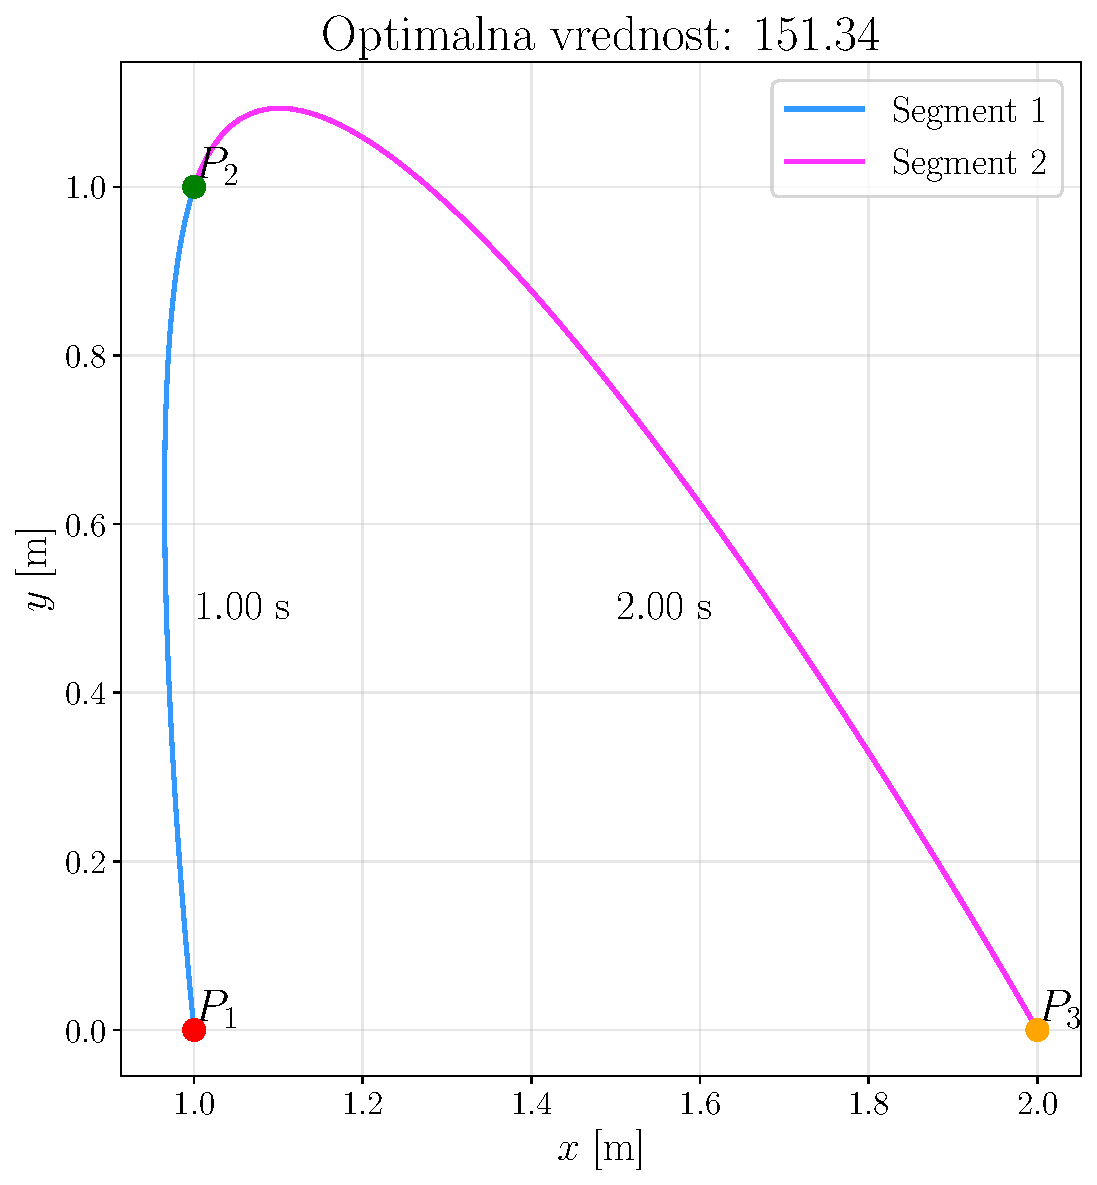
\includegraphics[width=0.6\textwidth]{images/trajectory_2d_qp.pdf}
    \caption{Trajektorija, dobljena z rešitvijo QP problema za $n = 2$ segmenta, $d = 4$, $K = 2$ in $r = 3$.}
    \label{fig:2segment}
\end{figure}

\subsection{Izračun gradienta}

Za izračun gradienta cenovne funkcije $F(\tvec)$ potrebujemo parcialne odvode matrike $\qmat$ in $\amat$ glede na časovne spremenljivke $t_1$ in $t_2$. V tem razdelku predstavimo te parcialne odvode v simbolični in numerični obliki.

V simbolični obliki:
\begin{equation}
\partial_{t_1}\mathbf{Q}(\tvec) = 
\begin{bNiceMatrix}[columns-width=auto]
\textcolor{block1color}{0} & \textcolor{block1color}{0} & \textcolor{block1color}{0} & \textcolor{block1color}{0} & \textcolor{block1color}{0} & 0 & 0 & 0 & 0 & 0 \\
\textcolor{block1color}{0} & \textcolor{block1color}{0} & \textcolor{block1color}{0} & \textcolor{block1color}{0} & \textcolor{block1color}{0} & 0 & 0 & 0 & 0 & 0 \\
\textcolor{block1color}{0} & \textcolor{block1color}{0} & \textcolor{block1color}{0} & \textcolor{block1color}{0} & \textcolor{block1color}{0} & 0 & 0 & 0 & 0 & 0 \\
\textcolor{block1color}{0} & \textcolor{block1color}{0} & \textcolor{block1color}{0} & \textcolor{block1color}{36} & \textcolor{block1color}{144 t_1} & 0 & 0 & 0 & 0 & 0 \\
\textcolor{block1color}{0} & \textcolor{block1color}{0} & \textcolor{block1color}{0} & \textcolor{block1color}{144 t_1} & \textcolor{block1color}{576 t_1^2} & 0 & 0 & 0 & 0 & 0 \\
0 & 0 & 0 & 0 & 0 & \textcolor{block2color}{0} & \textcolor{block2color}{0} & \textcolor{block2color}{0} & \textcolor{block2color}{0} & \textcolor{block2color}{0} \\
0 & 0 & 0 & 0 & 0 & \textcolor{block2color}{0} & \textcolor{block2color}{0} & \textcolor{block2color}{0} & \textcolor{block2color}{0} & \textcolor{block2color}{0} \\
0 & 0 & 0 & 0 & 0 & \textcolor{block2color}{0} & \textcolor{block2color}{0} & \textcolor{block2color}{0} & \textcolor{block2color}{0} & \textcolor{block2color}{0} \\
0 & 0 & 0 & 0 & 0 & \textcolor{block2color}{0} & \textcolor{block2color}{0} & \textcolor{block2color}{0} & \textcolor{block2color}{0} & \textcolor{block2color}{0} \\
0 & 0 & 0 & 0 & 0 & \textcolor{block2color}{0} & \textcolor{block2color}{0} & \textcolor{block2color}{0} & \textcolor{block2color}{0} & \textcolor{block2color}{0}
\end{bNiceMatrix}
\end{equation}

V numerični obliki pri $t_1 = 1, t_2 = 2$:
\begin{equation}
\partial_{t_1}\mathbf{Q}(1, 2) = 
\begin{bNiceMatrix}[columns-width=1.2em]
\textcolor{block1color}{0} & \textcolor{block1color}{0} & \textcolor{block1color}{0} & \textcolor{block1color}{0} & \textcolor{block1color}{0} & 0 & 0 & 0 & 0 & 0 \\
\textcolor{block1color}{0} & \textcolor{block1color}{0} & \textcolor{block1color}{0} & \textcolor{block1color}{0} & \textcolor{block1color}{0} & 0 & 0 & 0 & 0 & 0 \\
\textcolor{block1color}{0} & \textcolor{block1color}{0} & \textcolor{block1color}{0} & \textcolor{block1color}{0} & \textcolor{block1color}{0} & 0 & 0 & 0 & 0 & 0 \\
\textcolor{block1color}{0} & \textcolor{block1color}{0} & \textcolor{block1color}{0} & \textcolor{block1color}{36} & \textcolor{block1color}{144} & 0 & 0 & 0 & 0 & 0 \\
\textcolor{block1color}{0} & \textcolor{block1color}{0} & \textcolor{block1color}{0} & \textcolor{block1color}{144} & \textcolor{block1color}{576} & 0 & 0 & 0 & 0 & 0 \\
0 & 0 & 0 & 0 & 0 & \textcolor{block2color}{0} & \textcolor{block2color}{0} & \textcolor{block2color}{0} & \textcolor{block2color}{0} & \textcolor{block2color}{0} \\
0 & 0 & 0 & 0 & 0 & \textcolor{block2color}{0} & \textcolor{block2color}{0} & \textcolor{block2color}{0} & \textcolor{block2color}{0} & \textcolor{block2color}{0} \\
0 & 0 & 0 & 0 & 0 & \textcolor{block2color}{0} & \textcolor{block2color}{0} & \textcolor{block2color}{0} & \textcolor{block2color}{0} & \textcolor{block2color}{0} \\
0 & 0 & 0 & 0 & 0 & \textcolor{block2color}{0} & \textcolor{block2color}{0} & \textcolor{block2color}{0} & \textcolor{block2color}{0} & \textcolor{block2color}{0} \\
0 & 0 & 0 & 0 & 0 & \textcolor{block2color}{0} & \textcolor{block2color}{0} & \textcolor{block2color}{0} & \textcolor{block2color}{0} & \textcolor{block2color}{0}
\end{bNiceMatrix}
\end{equation}

V simbolični obliki:
{\footnotesize
\begin{equation}
\partial_{t_1}\amat(\tvec) = 
\begin{bNiceMatrix}[columns-width=0.5em]
\textcolor{block3color}{0} & \textcolor{block3color}{0} & \textcolor{block3color}{0} & \textcolor{block3color}{0} & \textcolor{block3color}{0} & 0 & 0 & 0 & 0 & 0 \\
\textcolor{block3color}{0} & \textcolor{block3color}{0} & \textcolor{block3color}{0} & \textcolor{block3color}{0} & \textcolor{block3color}{0} & 0 & 0 & 0 & 0 & 0 \\
\textcolor{block3color}{0} & \textcolor{block3color}{0} & \textcolor{block3color}{0} & \textcolor{block3color}{0} & \textcolor{block3color}{0} & 0 & 0 & 0 & 0 & 0 \\
\textcolor{block4color}{0} & \textcolor{block4color}{1} & \textcolor{block4color}{2 t_1} & \textcolor{block4color}{3 t_1^2} & \textcolor{block4color}{4 t_1^3} & \textcolor{block5color}{0} & \textcolor{block5color}{0} & \textcolor{block5color}{0} & \textcolor{block5color}{0} & \textcolor{block5color}{0} \\
\textcolor{block4color}{0} & \textcolor{block4color}{0} & \textcolor{block4color}{2} & \textcolor{block4color}{6 t_1} & \textcolor{block4color}{12 t_1^2} & \textcolor{block5color}{0} & \textcolor{block5color}{0} & \textcolor{block5color}{0} & \textcolor{block5color}{0} & \textcolor{block5color}{0} \\
\textcolor{block4color}{0} & \textcolor{block4color}{0} & \textcolor{block4color}{0} & \textcolor{block4color}{6} & \textcolor{block4color}{24 t_1} & \textcolor{block5color}{0} & \textcolor{block5color}{0} & \textcolor{block5color}{0} & \textcolor{block5color}{0} & \textcolor{block5color}{0} \\
\textcolor{block4color}{0} & \textcolor{block4color}{0} & \textcolor{block4color}{0} & \textcolor{block4color}{0} & \textcolor{block4color}{0} & \textcolor{block5color}{0} & \textcolor{block5color}{0} & \textcolor{block5color}{0} & \textcolor{block5color}{0} & \textcolor{block5color}{0} \\
0 & 0 & 0 & 0 & 0 & \textcolor{block6color}{0} & \textcolor{block6color}{0} & \textcolor{block6color}{0} & \textcolor{block6color}{0} & \textcolor{block6color}{0} \\
0 & 0 & 0 & 0 & 0 & \textcolor{block6color}{0} & \textcolor{block6color}{0} & \textcolor{block6color}{0} & \textcolor{block6color}{0} & \textcolor{block6color}{0} \\
0 & 0 & 0 & 0 & 0 & \textcolor{block6color}{0} & \textcolor{block6color}{0} & \textcolor{block6color}{0} & \textcolor{block6color}{0} & \textcolor{block6color}{0}
\end{bNiceMatrix}
\end{equation}
}

V numerični obliki pri $t_1 = 1, t_2 = 2$:
\begin{equation}
\partial_{t_1}\amat(1, 2) = 
\begin{bNiceMatrix}[columns-width=1.2em]
\textcolor{block3color}{0} & \textcolor{block3color}{0} & \textcolor{block3color}{0} & \textcolor{block3color}{0} & \textcolor{block3color}{0} & 0 & 0 & 0 & 0 & 0 \\
\textcolor{block3color}{0} & \textcolor{block3color}{0} & \textcolor{block3color}{0} & \textcolor{block3color}{0} & \textcolor{block3color}{0} & 0 & 0 & 0 & 0 & 0 \\
\textcolor{block3color}{0} & \textcolor{block3color}{0} & \textcolor{block3color}{0} & \textcolor{block3color}{0} & \textcolor{block3color}{0} & 0 & 0 & 0 & 0 & 0 \\
\textcolor{block4color}{0} & \textcolor{block4color}{1} & \textcolor{block4color}{2} & \textcolor{block4color}{3} & \textcolor{block4color}{4} & \textcolor{block5color}{0} & \textcolor{block5color}{0} & \textcolor{block5color}{0} & \textcolor{block5color}{0} & \textcolor{block5color}{0} \\
\textcolor{block4color}{0} & \textcolor{block4color}{0} & \textcolor{block4color}{2} & \textcolor{block4color}{6} & \textcolor{block4color}{12} & \textcolor{block5color}{0} & \textcolor{block5color}{0} & \textcolor{block5color}{0} & \textcolor{block5color}{0} & \textcolor{block5color}{0} \\
\textcolor{block4color}{0} & \textcolor{block4color}{0} & \textcolor{block4color}{0} & \textcolor{block4color}{6} & \textcolor{block4color}{24} & \textcolor{block5color}{0} & \textcolor{block5color}{0} & \textcolor{block5color}{0} & \textcolor{block5color}{0} & \textcolor{block5color}{0} \\
\textcolor{block4color}{0} & \textcolor{block4color}{0} & \textcolor{block4color}{0} & \textcolor{block4color}{0} & \textcolor{block4color}{0} & \textcolor{block5color}{0} & \textcolor{block5color}{0} & \textcolor{block5color}{0} & \textcolor{block5color}{0} & \textcolor{block5color}{0} \\
0 & 0 & 0 & 0 & 0 & \textcolor{block6color}{0} & \textcolor{block6color}{0} & \textcolor{block6color}{0} & \textcolor{block6color}{0} & \textcolor{block6color}{0} \\
0 & 0 & 0 & 0 & 0 & \textcolor{block6color}{0} & \textcolor{block6color}{0} & \textcolor{block6color}{0} & \textcolor{block6color}{0} & \textcolor{block6color}{0} \\
0 & 0 & 0 & 0 & 0 & \textcolor{block6color}{0} & \textcolor{block6color}{0} & \textcolor{block6color}{0} & \textcolor{block6color}{0} & \textcolor{block6color}{0}
\end{bNiceMatrix}
\end{equation}

Sedaj lahko sestavimo parcialin odvod celotne KKT matrike $\kmat$:

\begin{equation}
\partial_{t_1} \kmat(\tvec) =
\begin{bmatrix}
    \partial_{t_1} \qmat(\tvec) & \partial_{t_1} \amat(\tvec)^\top \\
    \partial_{t_1} \amat(\tvec) & 0
\end{bmatrix},
\end{equation}

s tem pa izračunamo tudi parcialne odvode implicitne funkcije $\yimplicit_x$ (vektor polinomskih koeficientov in Lagrangeovih multiplikatorjev za dimenzijo $x$) glede na $t_1$:

\begin{equation}
\partial_{t_1} \yimplicit_x(\tvec) = -\kmat(\tvec)^{-1} (\partial_{t_1} \kmat(\tvec) \yimplicit_x(\tvec)).
\end{equation}

Spomnimo, da v implementaciji inverza matrike $\kmat$ nikoli ne izračunamo eksplicitno, temveč rešujemo sistem enačb.

Za naš primer pri $t_1 = 1, t_2 = 2$ lahko izračunamo numerično vrednost parcialnega odvoda $\partial_{t_1} \yimplicit_x(1, 2)$. Ker je $\yimplicit_x = (\aimplicit, \muimplicit)$, lahko rezultat razdelimo na komponenti:

\begin{equation}
\partial_{t_1} \aimplicit_x(1, 2) = 
\begin{bmatrix}
\textcolor{block1color}{0,0000} \\
\textcolor{block1color}{0,0000} \\
\textcolor{block1color}{0,0000} \\
\textcolor{block1color}{0,4436} \\
\textcolor{block1color}{-0,7770} \\
\textcolor{block2color}{0,0000} \\
\textcolor{block2color}{0.2220} \\
\textcolor{block2color}{-0,3330} \\
\textcolor{block2color}{0,1665} \\
\textcolor{block2color}{-0,0278}
\end{bmatrix}, \quad
\partial_{t_1} \muimplicit_x(1, 2) = 
\begin{bmatrix}
\textcolor{block3color}{123,9019} \\
\textcolor{block3color}{56,6124} \\
\textcolor{block3color}{4,9913} \\
\textcolor{block4color}{-123,9019} \\
\textcolor{block4color}{19,3175} \\
\textcolor{block4color}{5,6621} \\
\textcolor{block4color}{-143,8854} \\
\textcolor{block6color}{19,9835} \\
\textcolor{block6color}{-20,6496} \\
\textcolor{block6color}{6,9942}
\end{bmatrix}
\end{equation}

S pomočjo enačbe \eqref{eq:grad} lahko sedaj izračunamo komponento gradienta glede na $t_1$:
\begin{equation}
    \label{eq:grad_t1}
    \partial_{t_1} F_x(1, 2) = \aimplicit_x(1, 2)^\top \qmat (\partial_{t_1} \aimplicit_x(1, 2)) + \frac{1}{2} \aimplicit_x(1, 2)^\top (\partial_{t_1} \qmat(1, 2)) \aimplicit_x(1, 2) = -9,9835
\end{equation}

Na analogen način lahko izračunamo tudi $\partial_{t_2} F_x$, $\partial_{t_1} F_y$ in $\partial_{t_2} F_y$, s čimer dobimo celoten gradient $\nabla F(\tvec)$:

\begin{equation}
\nabla F(\tvec) = (\partial_{t_1} F_x, \partial_{t_2} F_x) + (\partial_{t_1} F_y, \partial_{t_2} F_y).
\end{equation}

Ko vse te korake izračunamo, dobimo vrednost gradienta v točki $\tvec = (1, 2)$, ki je:
\begin{equation}
\nabla F(1, 2) = (-495,5232, -130,6149)
\end{equation}

Opazimo lahko, da sta obe komponenti gradienta negativni, kar pomeni, da bi se s povečanjem časov $t_1$ in $t_2$ lahko znižala vrednost cenovne funkcije $F(\tvec)$. To je smiselno, saj daljši časovni intervali omogočajo manj agresivne trajektorije, kar vodi do nižje vrednosti funkcije $F(\tvec)$. Vendar pa bi, če bi uporabili ta gradient v optimizacijskem algoritmu, prekršili omejitev $\mathbf{1}^\top \tvec = T$ oz. $t_1 + t_2 = T$, zato moramo uporabiti projekcijo gradienta na hiperravnino. Ta postopek bomo na tem primeru predstavili v naslednjem razdelku.

\subsection{Projekcija gradienta in gradientni korak}

Določimo $T = 3$, kar pomeni, da imamo omejitev $t_1 + t_2 = 3$. Zato želimo gradient $\nabla F(\tvec)$ projicirati na hiperravnino, določeno z normalnim vektorjem $\mathbf{1} = (1, 1)$. Projekcija gradienta $\nabla F(\tvec)$ na to hiperravnino se izračuna po formuli \eqref{eq:projection}, njen rezultat pa je:
\begin{equation}
\nabla_{\text{proj}} F(1, 2) = (-182,4541, 182,4541)
\end{equation}

V implementaciji ta gradient še normaliziramo, da se izognemo prevelikim korakom, in izvedemo gradientni korak z velikostjo $\alpha = 1$:
\begin{equation}
    \tvec_1 = \tvec_0 - \alpha \frac{\nabla_{\text{proj}} F(\tvec_0)}{\|\nabla_{\text{proj}} F(\tvec_0)\|} = (1, 2) - (-0,7071,  0,7071) = (1,7071, 1,2929)
\end{equation}

$\tvec_1$ je nova točka v prostoru časov, ki leži na hiperravnini $t_1 + t_2 = 3$. Sedaj lahko postopek ponavljamo dokler želen kriterij za konvergenco ni izpolnjen. Na sliki~\ref{fig:2segment_bo} je prikazana trajektorija pri točki $\tvec^*$, ki je točka, kjer $F$ doseže lokalni minimum. 



\begin{figure}
    \centering
    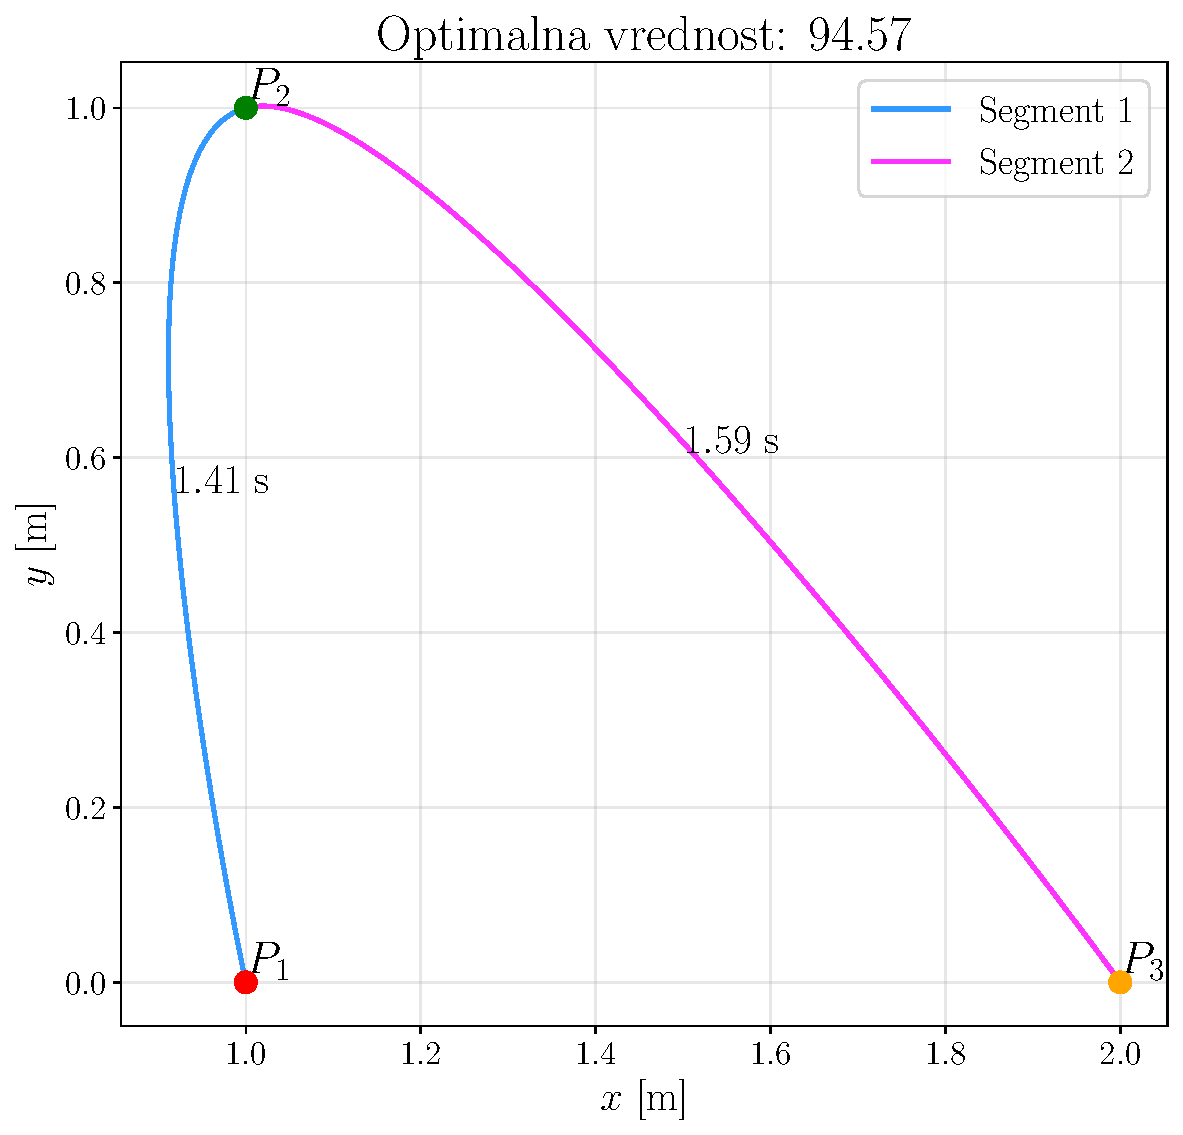
\includegraphics[width=0.6\textwidth]{images/trajectory_2d_bo.pdf}
    \caption{Trajektorija skozi tri vmesne točke pri časovnem vektorju $\tvec^*$.}
    \label{fig:2segment_bo}
\end{figure}




\section{Podrobnosti implementacije}
\label{app:implementation}
V tem dodatku se posvetimo podrobnostim implementacije hitrega izračuna analitičnega gradienta in Hessove matrike cenovne funkcije $F(\tvec)$. V prejšnjih poglavjih smo zavoljo jasnosti odvode različnih funkcij in matrik opisovali po komponentah (na primer, $\partial_{t_i} F$, $\partial_{t_i t_j} \aimplicit$, $\partial_{t_it_i} \qmat$, ...), vendar pa je v implementaciji smiselno uporabiti vektorizacijo in vektorske operacije, da se izognemo zankam in nepotrebnemu računanju z ničelnimi bloki. V tem dodatku bomo opisali, kako smo z vektorizacijo izračunali Hessovo matriko $\nabla^2 F(\tvec)$ in gradient $\nabla F(\tvec)$. Najprej predstavimo, kako smo prestrukturirali vhodne komponente algoritma~\ref{alg:gradhess} v tenzorje brez ničelnih blokov, nato pa s pomočjo tenzorjev in tenzorskih operacij opišemo, kako smo izračunali gradient in Hessovo matriko. Najprej pa na kratko predstavimo tenzorsko notacijo.

\subsection{Notacija}

V tem dodatku uporabljamo posebno notacijo za opis vektoriziranih operacij pri izračunu gradienta $\nabla F$. To nam omogoča, da kompaktno zapišemo operacije na tenzorjih, ki v implementaciji ustrezajo vektorskim operacijam brez eksplicitnih zank. Zato uvedemo nov simbol za sledečo operacijo: imamo tridimenzionalni tenzor $\mathcal{T} \in \mathbb{R}^{L_1 \times L_2 \times L_3}$ in matriko $\mathbf{M} \in \mathbb{R}^{L_3 \times L_2}$, želimo pa izračunati matriko $\mathbf{R} \in \mathbb{R}^{L_1 \times L_2}$, kjer je $R_i = \mathcal{T}_i M_i$. To operacijo označimo z $\mathcal{T} \times_1 \mathbf{M}$, kjer $\times_1$ označuje množenje po prvi dimenziji tenzorja \cite{kolda2009tensor}. 

\subsection{Vektorizacija vhodnih podatkov}
Kot vhodne podatke algoritma~\ref{alg:gradhess} imamo matriko $\qmat(\tvec)$, matriko $\amat(\tvec)$, vektorja $\avec^*$ in $\muvec^*$, nato pa izračunamo tudi parcialne odvode $\partial_{t_i}\qmat$, $\partial_{t_i} \amat$, $\partial_{t_it_j}\qmat$ in $\partial_{t_it_j}\amat$. Vse te matrike imajo redko strukturo, saj so sestavljene iz blokov, kjer je večina blokov ničelnih. V implementaciji smo te matrike prestrukturirali v tenzorje, kjer so shranjeni le neničelni bloki, kar nam omogoča, da z vektorskimi operacijami izračunamo vse parcialne odvode in komponente gradienta in Hessove matrike v enem klicu funkcije, brez zank po komponentah. Ti tenzorji so:

\begin{itemize}
    \item $\mathcal{Q'}$: tenzor velikosti $(n, d+1, d+1)$, kjer $n$ je število segmentov trajektorije in $d$ je stopnja polinoma. Ta tenzor vsebuje neničelne bloke parcialnih odvodov matrike $\qmat$. Velja $\mathcal{Q'}_i = \partial_{t_i} \qmat_i$ za $i=1,\ldots,n$.
    \item $\mathcal{A'}$: tenzor velikosti $(n, K+2, d+1)$, kjer $n$ je število segmentov trajektorije, $K$ je stopnja zveznosti in $d$ je stopnja polinoma. Ta tenzor vsebuje neničelne bloke parcialnih odvodov matrike $\amat$. Velja $\mathcal{A'}_i = \partial_{t_i} \amat_i$ za $i=1,\ldots,n$.\footnotemark[1]
    \item $\mathbf{X}$: matrika velikosti $(n, d+1)$, kjer je $n$ število segmentov trajektorije in $d$ je stopnja polinoma. Ta matrika vsebuje neničelne bloke vektorja $\avec^*$, kjer velja $\mathbf{X}_i = \avec^*_i$ za $i=1,\ldots,n$.
    \item $\mathbf{Y}$: matrika velikosti $(n, K+2)$, kjer je $n$ število segmentov trajektorije in $K$ je stopnja zveznosti. Ta matrika vsebuje neničelne bloke vektorja $\muvec^*$, kjer velja $\mathbf{Y}_i = \muvec^*_i$ za $i=1,\ldots,n$.
\end{itemize}

\footnotetext[1]{Striktno gledano imata bloka $\partial_{t_n} A_n$ in $\partial_{t_n t_n} A_n$ eno vrstico manj od ostalih blokov ($K+1$ vrstic, saj imamo pri ostalih blokih dodatno omejitev, ki določa skladanje končne koordinate z začetno v naslednjem segmentu), vendar pa smo v implementaciji dodali dodatno ničelno vrstico, da so vsi bloki enake velikosti in da lahko uporabimo vektorske operacije brez skrbi o različnih velikostih blokov.}

\subsection{Izračun gradienta}

Sedaj lahko z tenzorsko notacijo zapišemo sledečo matriko:

\begin{equation}
\mathbf{B}_{grad} = - \begin{bmatrix}
    \text{blkdiag}\left(\mathcal{Q'} \times_1 \mathbf{X}^T + \mathcal{A'} \times_1 \mathbf{Y}^T\right) \\
    \mathbf{0} \\
    \text{blkdiag}\left(\mathcal{A'} \times_1 \mathbf{X}^T\right)
\end{bmatrix}
\end{equation}

, kjer $i$-ti stolpec matrike $\mathbf{B}_{grad}$ predstavlja desno stran linearnega sistema, da izračunamo $\partial_{t_i} \yimplicit$. $\mathbf{0}$ je ničelna matrika velikosti $(K+1)\times n$. Simbol $\text{blkdiag}$ označuje operacijo bločne diagonalizacije iz tridimenzionalnega tenzorja dimenzij $k \times l \times m$ v bločno diagonalno matriko velikosti $k l \times k m$, kjer je $i$-ti element tenzorja (po prvi dimenziji) $i$-ti diagonalni blok v matriki. Z izračunom matrike $\mathbf{B}_{grad}$ se tako izognemo zankam po komponentah, kot smo to opisali v podpoglavju~\ref{sec:rhs}, in povečamo učinkovitost izračuna gradienta. Ko imamo matriko $\mathbf{B}_{grad}$, lahko rešimo sledeči sistem enačb:

\begin{equation}
\kmat \partial\yimplicit = \mathbf{B}_{grad},
\end{equation}
kjer je 
\begin{equation}
\partial \yimplicit = \begin{bmatrix} \partial_{t_1} \yimplicit & \partial_{t_2} \yimplicit & \cdots & \partial_{t_n} \yimplicit \end{bmatrix}.
\end{equation}

Matriko $\partial \yimplicit$ lahko nato uporabimo za izračun $\nabla F(\tvec)$, pa tudi kasneje za izračun desne strani linearnega sistema za izračun Hessove matrike $\nabla^2 F(\tvec)$. Tudi Hessovo matriko $\nabla^2 F(\tvec)$ izračunamo s pomočjo tenzorjev in Einsteinove sumacijske notacije, vendar pa je ta izračun nekoliko bolj zapleten, zato bralcu prepuščamo, da si ga ogleda v implementaciji (specifično v funkciji \texttt{build\_hess\_rhs} v datoteki \texttt{solver.py}).

\end{document}
